\documentclass[12pt,a4paper,twoside]{book}

% twoside for book style
%! compile with xelatex to allow reading the .eps files from parent directory
% when compiling with pdflatex, "epstopdf" cannot work on ../Plots/ due to
% security restrictions --> if pdflatex is needed (compiler error etc), copy
% Plots folder to this dir, then it should work.
% BETTER: run "pdflatex -shell-escape  main.tex" after 1st compilation fail and then before final compilation

% \usepackage[utf8]{inputenc}
    % only relevant for pdflatex

%! Colors
\usepackage{xcolor}
    \definecolor{shadecolor}{gray}{0.95}

%! images and figures
\usepackage{graphbox}
    % already loads graphicx package!
    % allows for "align=c" argument in includegraphics for aligning vertically

    \graphicspath{
        {fastImages}
        {../Plots/Thesis/1/}
        {../Plots/Thesis/2/}
        {../Plots/Thesis/3/}
        {../Plots/graphics/}
        {../Plots/photographs/}
    }
\usepackage{wrapfig}
    % allows wrapping text around figure; but has not so good performance
\usepackage[margin=10pt,font=small,labelfont={bf}]{caption}

%! layout
\usepackage{lmodern} % thicker font (?)
% \usepackage[inner=2.5cm,outer=3.5cm,top=2cm,bottom=2cm]{geometry}
%   for book style
\usepackage[inner=3cm,outer=3cm,top=2cm,bottom=2cm]{geometry}
%   for article style
\usepackage{booktabs}
\usepackage{multirow}
% \usepackage{ctable}
\usepackage{framed}
    % allows framing of text
% \usepackage{fancyhdr}
%     \pagestyle{fancy}
\vbadness=3000 % no warnings vor \vbox with badness < 2000

%! Typography
\usepackage[version=4]{mhchem}
    % chemistry
\usepackage{amssymb}
\usepackage{amsmath}

% units
\usepackage{siunitx}
    \DeclareSIUnit{\angstrom}{\textup{\AA}}
    \DeclareSIUnit{\bar}{bar}
    \DeclareSIUnit{\pulse}{pulse}
    \DeclareSIUnit{\wtpercent}{wt.\%}
    \sisetup{range-units=single}
    % \sisetup{range-phrase = \,--\,}

% greek
\usepackage{textgreek}
% lists
\usepackage{enumitem}
    % allows roman numbering
% quotes
\usepackage{csquotes}
    % convenient quotes

%! Referencing
% Table of contents
\setcounter{tocdepth}{3}
    % show subsubsection in ToC, 2 would only show until subsection
% \setcounter{secnumdepth}{3}
    % numering also subsubsections

% Glossary
\usepackage[acronym]{glossaries}
% \makeglossaries % run `makeglossaries main' in terminal then compile again
    \newacronym{tco}{TCO}{Transparent Conductive Oxide}
    \newacronym{uwbg}{UWBG}{Ultrawide-bandgap}

    \newacronym{xps}{XPS}{X-ray Photoelectron Spectroscopy}
    \newacronym{edx}{EDX}{Energy-dispersive X-Ray Spectroscopy}
    \newacronym{XRD}{XRD}{X-ray diffraction}
    \newacronym{AFM}{AFM}{Atomic Force Microscopy}
    \newacronym{RHEED}{RHEED}{Reflection High-Energy Electron Diffraction}

    \newacronym{vbm}{VBM}{Valence Band Maximum}
    \newacronym{cbm}{CBM}{Conduction Band Minimum}
    \newacronym{dft}{DFT}{Density Functional Theory}
    \newacronym{DOS}{DOS}{density of states}

    \newacronym{cvd}{CVD}{Chemical Vapor Deposition}
    \newacronym{pvd}{PVD}{Physical Vapor Deposition}
    \newacronym{pld}{PLD}{Pulsed Laser Deposition}
    \newacronym{mbe}{MBE}{Molecular Beam Epitaxy}
    \newacronym{hvpe}{HVPE}{Halide Vapor Phase Epitaxy}
    \newacronym{rf}{RF}{radio-frequency}
    \newacronym{dc}{DC}{direct current}

    % \newacronym{oop}{\textit{oop}}{out-of-plane}
    \newacronym{oop}{o.o.p.}{out-of-plane}
    % \newacronym{ip}{\textit{ip}}{in-plane}
    \newacronym{ip}{i.p.}{in-plane}
    \newacronym{FWHM}{FWHM}{Full Width at Half Maximum}
    \newacronym{RSM}{RSM}{Reciprocal Space Map}
    \newacronym{RMS}{RMS}{Root Mean Square}

    \newacronym{VCCS}{VCCS}{Vertical Continuous Composition Spread}
    \newacronym{DCS}{DCS}{Discrete Combinatorial Synthesis}

    \newacronym{UV}{UV}{ultra-violet}

    \newglossaryentry{pseudomorphic}{
        name = {pseudomorphic},
        description = {\tbd}
    }
    \newglossaryentry{bv}{
        name = {\textsc{Burger}'s vector},
        description = {\tbd}
    }
    \newglossaryentry{bl}{
        name = {\textsc{Bravais} lattice},
        description = {\tbd}
    }
    \newglossaryentry{bc}{
        name = {\textsc{Bragg} condition},
        description = {\tbd}
    }

% Links
\usepackage[colorlinks=true,citecolor=blue,linkcolor=violet]{hyperref}

%! own abbreviations
\newcommand{\agao}{\textalpha-\ce{Ga2O3}}
\newcommand{\cro}{\ce{Cr2O3}}

%! commenting in draft
\newcommand{\tbd}{\colorbox{magenta}{\emph{tbd}}}
\newcommand{\comment}[1]{
    \begin{shaded}
        \textsf{\underline{Comment}:
        \itshape\color{darkgray}
        #1
        }
    \end{shaded}
}

%! Library
\usepackage[style=numeric-comp,maxcitenames=2,sorting=none]{biblatex}
    %numeric-comp summerizes entries in \cite
\addbibresource{C:/Users/acdcj/OneDrive/Documents/Bibliothek/My Library.bib}
    \AtEveryBibitem{%
        \clearfield{month}%
        \clearfield{day}%
        \clearfield{urlyear}%
        \clearfield{urlmonth}%
        }
    \AtEveryCitekey{%
        \clearfield{month}%
        \clearfield{day}%
        \clearfield{urlyear}%
        \clearfield{urlmonth}%
        }

% Change the textcite command to "Name (year) [#]"
\usepackage{xpatch}
\xpatchbibmacro{textcite}
{\printnames{labelname}}
{\printnames{labelname} (\printfield{year})}
{}
{}

% \includeonly{tex-files/_chapters/Summary}

\begin{document}
%! Title Page
\newgeometry{inner=2.5cm,outer=2.5cm,top=2cm,bottom=2cm}
\thispagestyle{empty}
\begin{center}
        \vspace{0.5cm}
        \large
        Leipzig University\\
        Faculty of Physics and Earth System Sciences\\
        Semiconductor Physics Group\\[1.5cm]
        % \textbf{Leibniz-Institut für Oberfl\"achenmodifizierung e.V.}\\[2cm]
        \Huge
        \textbf{
            Structural and Electrical Properties of
            \texorpdfstring{\cro}{Cr2O3}
            Thin Films Grown by Pulsed Laser Deposition
            }\\[1.2cm]

        \includegraphics[width=0.7\textwidth]{uni logo.png}\\

        \vspace{.8cm}
        
    
        \LARGE
        Master's Thesis\\
        
            
        \vspace{1cm}

        \large
        Submitted by\\
        \LARGE
        \textbf{Jakob Seifert}\\[.5cm]
        \large
        Leipzig, November 2024
        
        \vfill
            
            
        \vspace{0.8cm}
            
            
        \large
        \centering
        \begin{tabular}{ll}
            \toprule
            Revision:       & Prof.\ Dr.\ Marius Grundmann\\
                            & Dr.\ habil.\ Holger von Wenckstern\\[1cm]
            Supervision:    & Dr.\ habil.\ Holger von Wenckstern\\
                            & Dr.\ Sofie Vogt\\
                            & Clemens Petersen
        \end{tabular}
        % Supervision:
        
        % Second Referee:
        
        
            
    \end{center}

\restoregeometry
\clearpage{\thispagestyle{empty}}
\cleardoublepage

%! TOC
% \dominitoc
\tableofcontents
\cleardoublepage


%! main text
    \chapter{Introduction}
%! Einordnung
Semiconductor technology today is based on the versatility of silicon: its band gap of \qty{1.1}{\eV} is large enough to allow tailoring its conductivity from semi-insulating to conductive -- on the other hand, it is small enough to enable both \textit{p}- and \textit{n}-type doping.
Even though being present in a vast range of applications, todays technological requirements push silicon to its limits:
power switching applications and high-frequency electronics are strongly dependent on the electrical field at which breakdown occurs
    \cite{higashiwaki2018}.
This critical field strength however is correlated to the band gap of the underlying material
    \cite{slobodyan2022},
which is why \acrfull{uwbg} materials have gained much attention:
Those semiconducors enable devices with smaller dimensions and reduced losses, which can provide the necessary properties which are needed, for example, in the optimization of charging and motor drive efficiency in electric vehicles
    \cite{gupta2024}
-- which itself is an important step towards lowering emissions.

One interesting \acrshort{uwbg} semiconductor is \gao, which turned out to be a viable material for solar-blind UV detectors
    \cite{singhpratiyush2017},
power rectifiers
    \cite{yang2017},
power MOSFETs
    \cite{moser2017}
and gas sensors
    \cite{ogita2001}.
% Its thermodynamically most stable \textbeta-phase ($E_g=4.6-\qty{5.0}{\eV}$) has been extensively studied,
Gallium oxide crystallizes in different polymorphs, of which the \textalpha-phase has the highest band gap of up to \qty{5.3}{\eV}
    \cite{hassa2021a}.
This metastable \gao\ phase crystallizes in the corundum structure, making it isostructural to cost-efficient and readily available sapphire (\alo) substrates.
However, there is still a lattice mismatch of \qty{4.6}{\percent} between \agao\ and \alo, regarding the $a$ lattice constant.
This introduces a large amount of threading dislocations
    \cite{kaneko2012},
which strongly reduces the electron mobiltiy in \agao\ thin films
    \cite{takane2023}.
Additionally, due to similar growth conditions of the \textbeta-phase, phase pure deposition of \agao\ is a challenge for different growth techniques
    \cite{bosi2020}.
Several attempts have been undertaken to improve the crystal quality and reduce the dislocation density in \agao\ thin films, namely epitaxial lateral overgrowth
    \cite{kawara2020}
and growth on patterned substrates
    \cite{nikolaev2020}
or buffer layers
    \cite{jinno2016,jinno2018}.

A promising buffer layer material for \agao\ is chromium oxide (\cro), which is isomorphic to \agao\ with a very low lattice mismatch of only \qty{0.4}{\percent} regarding the $a$ lattice constant -- one order of magnitude lower compared to \alo.
The feasibility of this approach has been demonstrated with \acrfull{hvpe}, a \acrfull{cvd} method, on \textit{c}-sapphire.
    \cite{stepanov2021,polyakov2022,polyakov2022a,butenko2023}.
\cro\ is also interesting due to its defect-induced \textit{p}-type nature, which can be enhanced by doping with lower valent cations
    \cite{arca2011,arca2013,arca2017,farrell2015}.
Because it is virtually impossible to achieve \textit{p}-type \gao\
    \cite{pearton2018},
\cro\ is a candidate for both \textit{p}-type alloys with \agao, similar to \ce{(Ir,Ga)2O3}
    \cite{kaneko2021},
and for \textit{p}-\textit{n} heterostructures with very low lattice mismatch at the interface
    \cite{polyakov2022a}.

%! aim of this work
Because \acrfull{pld} is a promising \acrfull{pvd} method for fabricating \agao\ thin films and devices
    \cite{petersen2023,vogt2023,vogt2024},
the aim of this work is to show the feasibility of preparing \cro\ thin films via \acrshort{pld}.
Therefore, the growth window of thin film growth depending on oxygen partial pressure, growth temperature and substrate orientation is investigated (chapter \ref{Sec:Results_Preliminary}).
Detailled structural analysis via \glspl{RSM} is done for thin films fabricated with various laser energy densities during the deposition (chapter \ref{Sec:Results_Energy}).
Furthermore, a segmented target approach is utilized to aim for tailored conductivities of Zn- and Cu-doped \cro\ thin films (chapter \ref{Sec:Results_Doping}).
Finally, it is demonstrated that \agao\ can be deposited phase pure on \cro\ buffer layers in \textit{c}-, \textit{r}-, \textit{m}- and \textit{a}-orientation (chapter \ref{Sec:Results_Buffer}).
Before analyzing the results of those experiments, a short overview will be given on the here investigated sesquioxides, as well as the basics of \acrfull{XRD} and heteroepitaxy of rhombohedral materials.
        \cleardoublepage
    \chapter{Theory}

\section{X-ray Diffraction Principles}
    \subsection{Scattering at Lattices}
To elucidate the working principles behind \gls{XRD} as a measurement method (cf.~\ref{Sec:Methods_XRD}), a brief description of reciprocal space and constructive interference will be provided.
Those derivations are based on \textcite{ashcroft1976}.

A periodic point-like structure with translational symmetry (\enquote{\gls{bl}}) can be described by three vectors $\mathbf{a}_i$ that span a so-called \enquote{unit cell}.
Every lattice point $\mathbf{R}$ is a linear combination of those unit cell vectors.
For such a lattice, there exists a so-called \enquote{reciprocal lattice}, which consists of all vectors $\mathbf{K}$ satisfying the condition\footnote{
    The definition of $\textbf{K}$ by (\ref{equ:Theory_DefReciprocal}) is a consequence of demanding that the plane wave described by $f_\mathbf{K}(\mathbf{r})=\exp(i\langle\mathbf{K},\mathbf{r}\rangle)$ has the same symmetry as the \gls{bl}
        \cite{ashcroft1976}.
}:
\begin{equation}\label{equ:Theory_DefReciprocal}
    e^{i\langle\mathbf{K},\mathbf{R}\rangle}=1\,.
\end{equation}
This is again a \gls{bl} with unit cell vectors $\mathbf{a}_j^*$:
\begin{equation}
    \mathbf{K}_{hkl}=h\mathbf{a}_1^*+k\mathbf{a}_2^*+l\mathbf{a}_3^*\,.
\end{equation}
It follows that for any $i,j$:
\begin{equation}
    \langle\mathbf{a}_i^*,\mathbf{a}_j\rangle=2\pi\delta_{ij}\,,
\end{equation}
with the \textsc{Kronecker} delta $\delta_{ij}$.
A major application of reciprocal space vectors is their ability to describe lattice planes.
Any lattice plane can be described by the shortest possible reciprocal space vector $\mathbf{K}_{hkl}$ perpendicular to it.
Consequently, the lattice plane is denoted by $(hkl)$.
The distance between equivalent lattice planes can be calculated via
\begin{equation}\label{Equ:Theory_planeDistance}
    d_{hkl}=|\mathbf{K}_{hkl}|^{-1}\,.
\end{equation}
Note that for non-cubic crystals, the lattice plane (hkl) is in general \textit{not} perpendicular to the lattice direction [hkl].

With those preliminarities, the conditions for constructive interference during dif\-frac\-tion of radiation at \glspl{bl} can be derived.
Consider two scattering centers separated by $\mathbf{d}$.
Now consider incoming radiation with wave vector $\mathbf{k}$:
\begin{equation}
        \mathbf{k}=\frac{2\pi}{\lambda}\hat{\mathbf{n}}\,,
\end{equation}
with wavelength $\lambda$ and direction $\hat{\mathbf{n}}$.
For the case of elastic scattering, the outcoming wave vector $\mathbf{k}'$ has the same wavelength $\lambda$ but different direction $\hat{\mathbf{n}}'$.
The phase difference of two photons scattered at the 1st and 2nd scattering center, respectively, can be calculated from their path difference, which reads
\begin{equation}\label{Equ:Theory_PathDifference}
    \langle\mathbf{d},\hat{\mathbf{n}}\rangle+\langle-\mathbf{d},\hat{\mathbf{n}}'\rangle\,.
\end{equation}
\begin{figure}
    \centering
    \includegraphics[width=.5\textwidth]{example-image-a}
    \caption{\textit{Here comes an ashcroft-like image for the scattering geometry to derive Equ.~(\ref{Equ:Theory_PathDifference})}}
\end{figure}
Constructive interference occurs, if the phase difference is an integral multiple of the wavelength, so it must follow that
\begin{align}
    \langle\mathbf{d},(\hat{\mathbf{n}}-\hat{\mathbf{n}}')\rangle&=m\lambda\\
    \Leftrightarrow\langle\mathbf{d},(\hat{\mathbf{k}}-\hat{\mathbf{k}}')\rangle&=2\pi m\,,
    \label{Equ:Theory_ConstructiveInterference}
\end{align}
with $m\in\mathbb{N}$.
Comparing with \eqref{equ:Theory_DefReciprocal} reveals that $\hat{\mathbf{k}}-\hat{\mathbf{k}}'$ is a reciprocal space vector, because the separation $\mathbf{d}$ of the two scattering centers is a lattice vector.
So constructive interference (observing a reflex) occurs if and only if the scattering geometry (determined by angle of incidence and refraction, as well as wavelength) matches the lattice symmetry in the sense that there is a corresponding lattice translation vector $\mathbf{d}$ fulfilling \eqref{Equ:Theory_ConstructiveInterference}.
So from the \enquote{position} of reflexes, one can deduce the lattice symmetry.

Note that this description of X-ray scattering is equivalent to the \gls{bc}:
\begin{equation}\label{Equ:Theory_BraggCondition}
    m\lambda=2d_{hkl}\sin(\theta)\,,
\end{equation}
where the angle of incidence $\theta$ and $\lambda$ are contained in $\hat{\mathbf{k}}-\hat{\mathbf{k}}'$.
Furthermore, when a lattice point is not equivalent to a single atom, but represents several scattering centers, an additional geometrical structure factor has to be taken into account to determine whether a certain geometry allows reflexes.
This is important, e.g., for structures with trigonal symmetry. 
They are described with a conventional hexagonal unit cell, although not every plane $(hkl)$ exhibits constructive interference.

\subsection{X-rays}\label{Sec:Theory_XRays}
Atomic distances in solids are of the order of several \si{\angstrom}, so the radiation for probing those structures must have a similar wavelength, which turns out to be X-rays
    \cite{harrington2021}.
The following description of X-rays is based on \textcite{spiess2009}.

The basis of any X-ray tube are high-energy electrons which are produced by thermionic emission in a cathode, which is usally made out of tungsten\footnote{
    Tungsten is the element with the second highest melting point of around \qty{3400}{\celsius}.
    This ensures a low contamination of the anode with cathode material.
}.
An electric field of several \si{\kV} accelerates the electrons to the anode, where they are stopped such that around \qty{99}{\percent} of their kinetic energy dissipates.
The momentum change of electrons, which are charged particles, leads to emission of \textit{bremsstrahlung}.
Furthermore, the electrons ionize atoms of the anode material which leads to unoccupied electron states.
If those states are filled by electrons with higher quantum number $n$, the difference in energy of those levels is emitted as radiation with a discrete spectrum, called characteristic X-ray.
Important for this work is a part of the characteristic spectrum, called K-radiation, which originates in occupation of empty $1s$-orbitals.
The occupying electron must come from an orbital with angular momentum quantum number $l=1$, i.e.\ a \textit{p}-orbital, because $\Delta l$ cannot be zero.
The radiation is termed K\textalpha- or K\textbeta-radiation, if the previous orbital was $2p$ or $3p$, respectively.
Furthermore, one distinguishes K\textalpha\textsubscript{1}- and K\textalpha\textsubscript{2}-radiation, depending on the magnetic quantum number of the previous orbital, which can be $\frac{3}{2}$ or $\frac{1}{2}$, respectively.
K\textalpha-radiation is desired for probing crystal structures.
        \label{Sec:Theory_X-ray_diffraction}

\section{Sesquioxides}
    \glspl{tco} are materials that combine the properties of having low absorption coefficient in the visible spectrum and being conductive at the same time
    \cite{kehoe2016}.
The interest in these materials is motivated by possible usage in portable and flexible electronics, displays, solar cells and more
    \cite{ginley2011}.
Due to the restriction on only a few materials in the industry (e.g. \ce{SnO2} and \ce{In2O3}), investigations of new materials are required
    \cite{ginley2011}.
This includes fabrication of \textit{p}-type \glspl{tco} as well as compounds with even larger band gaps than \qty{3}{eV}, called \gls{uwbg} materials.
A candidate for the latter is \ce{Ga2O3} with its several polymorphs
    \cite{hassa2021a},
where the corundum structured \agao{} gained interest, even though its deposition has to account for parasitic growth of the thermodynamically more stable \textbeta-phase
    \cite{petersen2023}.

At this point, \ce{Cr2O3} comes in handy being a possible \textit{p}-type \gls{tco} as well as being isomorphic to group-III sesquioxide \agao{} with quite similar lattice parameters (cf. Tab.\,\ref{Tab:sesquiLatticeConstants}).
This enables the use of \ce{Cr2O3} as a buffer layer between \agao{} and isomorphic \textalpha-\ce{Al2O3} (sapphire) substrates to improve the deposition process
    \cite{stepanov2021}.
Furthermore, \ce{Cr2O3} exhibits increased conductivity upon doping
    \cite{uekawa1996}
and could thus serve as \textit{p}-type component in a \textit{p}-\textit{n}-heterojunction with \agao{}.
In the following, an overview of the two mentioned sesquioxides will be provided with focus on the physical properties being relevant to this work.
    \subsection{Chromium Oxide}\label{Sec:Cr2O3}
        % ----------------------
% --- chromium oxide ---
% ----------------------

\enquote{Chromia} or \enquote{Eskolaite} is a sesquioxide composed of the transition metal chro\-mi\-um and oxygen with formula unit \ce{Cr2O3}.
Among other chromium oxides (e.g. metallic \ce{CrO2}, toxic \ce{CrO3} etc.), it is the thermodynamically most stable phase 
    \cite{lebreau2014,robbert1998,al-kuhaili2007},
making it the abundant chromium oxide on earth
    \cite{mi2018}.
\ce{Cr2O3} occurs mainly in the \textalpha-phase (described below), but a cubic spinel \textgamma-phase with random missing \ce{Cr} point defects has also been reported
    \cite{robbert1998}.
Henceforth, \enquote{\ce{Cr2O3}} will refer to the \textalpha-phase.

% Miscellaneous
As coating material, \ce{Cr2O3} is commonly used due to its high hardness and resistance against corrison \cite{singh2019,al-kuhaili2007}, also explaining its use-case as component of stainless steel to form passive films \cite{lebreau2014}.
\ce{Cr2O3} thin films absorb electromagnetic waves with wavelengths smaller than \qty{400}{\nm}, making it opaque in the \acrshort{UV}-spectrum \cite{cheng1996,guillen2021}.
It is transparent in the visible spectrum with, e.g., a reported transmittance of \qty{40}{\percent} at \qty{700}{\nm} for \qty{0.5}{\um} thick films by \citeauthor{cheng1996}~(\citeyear{cheng1996}) \cite{cheng1996}.

% crystal structure
\ce{Cr2O3} crystallizes in the corundum structure, which has trigonal symmetry (space group $R\bar{3}c$) and belongs to the hexagonal crystal family.
One unit cell contains six formula units, i.e. 12 chromium cations and 18 oxygen anions
    \cite{lebreau2014}.
The oxygen atoms arrange in a hexagonal close-packed manner, where two thirds of the formed octahedrons are filled with \ce{Cr} atoms
    \cite{catti1996}.
The unit cell is spanned by a principal axis, called \textit{c}-axis\footnote{The spins of the \ce{Cr} atoms along this direction are alternating $3\uparrow$ and $3\downarrow$ \cite{kehoe2016}, making the crystal antiferromagnetic \cite{catti1996,lebreau2014}.}, and a hexagonal basal plane with lattice constant \textit{a}.
The numerical values for those lattice parameters differ depending on the publication \cite{finger1980,arca2013,kehoe2016,mi2018,stepanov2021}, and we will use the values in Tab.~\ref{Tab:sesquiLatticeConstants}.
\begin{table}
    \centering
    \begin{tabular}{ccc|l}
        &\textit{a}&\textit{c}&Ref.\\\hline
        \textalpha-\ce{Al2O3}&&&\\
        \textalpha-\ce{Cr2O3}&$\qty{4.96}{\angstrom}$&$\qty{13.59}{\angstrom}$&\citeauthor{mi2018} (\citeyear{mi2018}) \cite{mi2018}\\
        \textalpha-\ce{Ga2O3}&&
    \end{tabular}
    \caption{Lattice constants of selected corundum structured compounds.}
    \label{Tab:sesquiLatticeConstants}
\end{table}

% growth techniques
Several techniques were applied for depositing chromia thin films, including:
\gls{cvd}
    \cite{cheng2000,cheng2001a,cheng2001}
    on silicon and glass,
\gls{mbe} on sapphire
    \cite{farrell2015,kehoe2016},
thermal evaporation on platinum
    \cite{robbert1998},
electron-beam evaporation on glass
    \cite{al-kuhaili2007},
spray porylisis on glass
    \cite{arca2011},
\gls{rf} sputtering on sapphire
    \cite{stepanov2021,polyakov2022a,polyakov2022},
reactive \gls{dc} sputtering on glass
    \cite{guillen2021},
reactive \gls{pld} on silicon
    \cite{caricato2010}
and sapphire
    \cite{punugupati2015},
and non-reactive \gls{pld} on sapphire
    \cite{singh2019,arca2017,kehoe2016}.

% ----------------------------
% --- electronic structure ---
% ----------------------------
\paragraph{Electronic Structure}
Experimental and theoretical studies reveal that chromia exhibits a band gap of \qtyrange{3.2}{3.4}{\eV}
    \cite{mi2018,robbert1998,lebreau2014,arca2013}
making it a wide band gap material.
% Numerical calculations locate the smallest direct band gap at the $M$-point (Brillouin zone edge in $\langle10.0\rangle$-direction).
This predicts insulating behavior \cite{arca2013}, classified as both Mott-Hubbard type and charge-transfer type, which are models to describe the electronic behavior of compounds containing transition metals with partly filled $3d^n$ orbitals\footnote{$n=5$ for \ce{Cr}}
    \cite{catti1996,mi2018,lebreau2014}:
\gls{dft} calculations show that the \ce{Cr}-$3d$ states are almost solely responsible for electronic states in the conduction band and that they are also present in the valence band
    \cite{mi2018,lebreau2014}.
Thus, $3d\longrightarrow 3d$ band transitions are possible, favoring the Mott-Hubbard model of this compound
    \cite{lebreau2014}.
Furthermore, the \ce{O}-$2p$ states are mainly present in the valence band, at similar energies as the \ce{Cr}-$3d$ states, which leads to hybridization and thus favoring the charge-transfer model
    \cite{lebreau2014}.

% p-type of undoped Cr2O3 due to defects
However, several studies agree on \ce{Cr2O3} being a semiconductor with \textit{p}-type conductivity\footnote{
    \citeauthor{cheng2001a} (\citeyear{cheng2001a}) actually find \ce{Cr2O3} to be insulating. It is noted that they examined \ce{Cr2O3} as an \qty{2}{\nm} thick oxide surface on \ce{CrO2} films deposited by \gls{cvd} \cite{cheng2001a}.
    \citeauthor{farrell2015} (\citeyear{farrell2015}) also find that their high quality epitaxial films of \ce{Cr2O3} grown by \gls{mbe} exhibit no \textit{p}-type conductivity \cite{farrell2015}.
    Similar results were found by \citeauthor{kehoe2016} (\citeyear{kehoe2016}) for \gls{mbe} and \gls{pld} deposited films \cite{kehoe2016}.
}
at room temperature and atmospheric conditions
    \cite{kofstad1980,cheng1996,caricato2010,lebreau2014,mi2018,singh2019,polyakov2022a}.
Calculating the impact of different crystal point defects on the band structure may give insight into these observations.
Indeed, when considering a missing chromium atom (\enquote{vacancy} $V_{\ce{Cr}}$) the band structure changes in two ways:
The band gap itself is reduced \cite{mi2018}, but not in a way that it would make excitations of valence electrons into the conduction band much more probable than at room temperature.
But additionally, there is a new band introduced slightly above the Fermi level (cf. Fig.~\ref{Fig:lebreau2014_acceptorLevel}), which acts as an unoccupied acceptor level
    \cite{mi2018}.
This defect state is mainly composed of \ce{O}-$2p$ orbitals of the oxygen anions surrounding the vacancy
    \cite{lebreau2014}.
From a more intuitive point of view, a missing neutral chromium atom effectively removes the \ce{Cr^3+} cation as well as three electrons bound to the adjacent \ce{O^2-} anions, thus creating three holes \cite{lebreau2014} explaining the \textit{p}-type conductivity.
\begin{figure}
    \centering
    \includegraphics[width=.5\textwidth]{lebreau2014_acceptorLevel}
    \caption{Calculated \acrfull{DOS} of chromia, taking a $V_{\ce{Cr}}$ into account.
    The arrow marks the new acceptor level.
    Image taken from \cite{lebreau2014}.}
    \label{Fig:lebreau2014_acceptorLevel}
\end{figure}

Note that there are also other possible defects with different effects:
a chromium Frenkel point defect describes a \ce{Cr} atom leaving it's position and occupying a formerly unoccupied cavity in one of the oxygen-octahedrons.
This Frenkel defect actually creates a new band right below the Fermi level, acting as an occupied donor level
    \cite{lebreau2014}.
A similar defect state is introduced by oxygen vacancies
    \cite{mi2018}.
But note that the Fermi level is located only slightly above the \gls{vbm} and thus the new occupied donor level is not significantly closer to the \gls{cbm}, which means that electrons still have to overcome the band gap energy to get into conducting states.
This favors the formation of holes via \ce{Cr} vacancies (\ce{O}-$2p$ acceptor states) rather than electrons via \ce{Cr} Frenkel defects and \ce{O} vacancies (\ce{Cr}-$3d$ donor states).

% --- Doping ---
\paragraph{Doping}
Several attempts have been made to alter the conductivity of chromia thin films, including incorporation of magnesium, nickel, or lithium to achieve better \textit{p}-type conductivity
    \cite{farrell2015}.
On the other hand, incorporating titanium seems to yield electrons as majority carriers 
    \cite{holt1994}
due to the higher valent state of \ce{Ti} when substituting \ce{Cr} sites (\ce{Ti_{Cr}})
    \cite{kofstad1980}.

Due to interest in the electrical properties of \textit{p}-type \glspl{tco}, the influence on \ce{Mg}-doped \ce{Cr2O3} thin films has been investigated by several studies
    \cite{holt1994,uekawa1996,arca2011,arca2013,farrell2015,arca2017,kehoe2016}.
Substituting \ce{Cr} atoms with less valent hole providers -- compared to structural defects of pure \ce{Cr2O3} -- does not only allow for a more controlled defect incorporation, but is also energetically more favorable due to a lower formation energy of \ce{Mg_{Cr}} compared to $V_{\ce{Cr}}$
    \cite{kehoe2016}.
\citeauthor{uekawa1996} (\citeyear{uekawa1996}) report an increase in conductivity of five orders of magnitude for \ce{Cr2O3{:}Mg} thin films
    \cite{uekawa1996}.
This result can be further improved by postannealing
    \cite{farrell2015}
and deposition at higher oxygen partial pressures
    \cite{holt1994,farrell2015}.
These effects are attributed to homogenization of magnesium inside the thin films and increased \ce{MgO} incorporation during deposition, respectively.
An observed side-effect of \ce{Mg}-doping is a color change to a brownish tint
    \cite{uekawa1996,arca2013}.
\Citeauthor{uekawa1996} (\citeyear{uekawa1996}) discuss that this may be the result of a mixed valence state of chromium (\ce{Cr^4+} or \ce{Cr^6+}), formed upon doping, as observed by \gls{xps}.
This may establish an unoccupied state, favoring charge-transfer transitions from \ce{O}-$2p$ orbitals to this low-energetic state, resulting in a different visual appearence of the thin films.
However, it has been shown that the overall transparency can be increased by codoping of \ce{Mg} with nitrogen which also reduces the decolorization substantially
    \cite{arca2011,arca2013}.
    \subsection{Gallium Oxide}
        \ce{Ga2O3} is a group-III sesquioxide with four different polymorphs, of which \textbeta-\ce{Ga2O3} is the thermodynamically most stable one at ambient conditions
    \cite{schewski2015,hassa2021a,petersen2023}.
The corundum-structured \agao{} phase, which is of more relevance for this work, is isomorphic to \ce{Cr2O3} (cf.~\ref{Sec:Cr2O3}), with lattice parameters as listed in Tab.\,\ref{Tab:sesquiLatticeConstants}.
\agao{} is metastable
    \cite{kaneko2023},
i.e. not favored in the first place, but remains irreversibly after formation, e.g., after phase transition from \textbeta- to \textalpha-phase at high temperatures
    \cite{pearton2018}.
The thermodynamic equilibrium -- which determines the favored phase -- can also be changed by strain due to lattice mismatch occurring during heteroepitaxy\footnote{
    However, the possibility of formation of parasitic \textbeta-phase still has to be taken into account
        \cite{petersen2023}.
    }
    \cite{schewski2015}.
This approach is of particular interest due to the possibility of deposition on cheap\footnote{
    Compared to bulk \textbeta-\ce{Ga2O3} substrates
        \cite{yang2022,kaneko2023}.
}
and readily available sapphire substrates which are isomorphic to \agao{}
    \cite{pearton2018,polyakov2022,kaneko2023}.
Note that deposition of \textbeta-\ce{Ga2O3} on sapphire is also possible, but only with restriction to formation of more than one crystal domain
    \cite{yang2022}.
On the other hand, highly crystalline
    \cite{pearton2018}
\agao{} thin films should be able to be grown without rotational domains
    \cite{yang2022}.

Deposition of \agao{} on sapphire has been done by several deposition techniques, including \cite{yang2022}:
    \gls{hvpe},
    mist \gls{cvd}
        \cite{kaneko2012},
    \gls{mbe}
        \cite{schewski2015},
    Atomic Layer Deposition and
    metalorganic \gls{cvd}.
Phase-pure deposition via \gls{pld} has also been achieved
    \cite{schewski2015,petersen2023}.
Despite being isomorphic to each other, \agao{} and sapphire still exhibit a lattice mismatch of around \qty{4.8}{\percent} along the \textit{a}-axis
    \cite{kaneko2023}.
This induces semicoherent growth with a fairly high dislocation density, which has been reported to be around \qty{7e10}{\per\square\cm}
    \cite{kaneko2012}.
In particular, this becomes a problem regarding carrier mobility which is tremendously hindered by dislocation scattering
    \cite{kaneko2023}.

To overcome the problems of lattice mismatch between sapphire substrates and \agao{} thin films, quasi-continuous gradients from \ce{Al2O3} to \agao{} have been applied, utilizing the capability of alloying the respective compounds
    \cite{jinno2016}.
Furthermore, buffer layers of isomorphic \ce{Cr2O3} have been used to decrease the high dislocation density for deposition on \textit{c}-oriented
    \cite{stepanov2021,polyakov2022a}
as well as \textit{r}-oriented sapphire
    \cite{polyakov2022}.
Deposition on other than \textit{c}-oriented substrates also seems to decrease parasitic phases, because the suppression of crystal facets perpendicular to the principal \textit{c}-axis may increase phase purity
    \cite{jinno2021}.
It has to be noted that despite the difficulties occuring upon lattice mismatch, coherent growth seems to be feasible without buffer layers for different deposition techniques, at least for some monolayers
    \cite{schewski2015}.

% --- electronic structure ---
With \qtyrange{5.0}{5.3}{\eV}
    \cite{yang2022},
\agao{} has the highest band gap of the four polymorphs
    \cite{pearton2018}.
Increasing or decreasing the band gap is possible by alloying with \ce{Al2O3}
    \cite{jinno2021}
or \ce{In2O3}
    \cite{hassa2020},
respectively.
The crystal structure also allows for alloying with other corundum structured compounds
    \cite{yang2022},
in particular other transition metal oxides such as \ce{Cr2O3}
    \cite{polyakov2022,polyakov2022a}.
The conduction band is mainly composed of \ce{Ga}-$4s$ states with an effective electron mass of \qty{0.3}{m_e}.
The valence band is very flat and mainly composed of \ce{O}-$2p$ orbitals, yielding a high effective electron mass and thus strong localization
    \cite{pearton2018}.
Next to band gap engineering, \textit{n}-type doping via \ce{Sn} or \ce{Si} incorporation has been accomplished
    \cite{yang2022}.


\section{Heteroepitaxy}
    %!
\subsection{Pseudomorphic Growth}
\label{sec:Theory_PseudomorphicGrowth}
% \comment{
%     Ist der folgende Absatz zu lang, dafür dass ich (wahrscheinlich) nur bei \emph{c}-Orientierung pseudomorphic growth beobachte?
%     Aber ich wollte gerne ausrechnen, was denn der out of plane strain \emph{wäre}, falls es so sein sollte, damit ich später argumentieren kann, ob ich relaxed oder pseudomorphic beobachte; oder was dazwischen.
%     Dementsprechend hab ich mich dann gezwungen gefühlt, das ganze noch mal aufzurollen.
%     Vielleicht wäre eine Lösung, (\ref{euq:e3-a}), (\ref{euq:e3-m}) und (\ref{euq:e3-c}) in eine Art appendix zu tun?
%     }
When a body is deformed (\emph{strained}) from its original state of equilibrium (\emph{bulk}), forces will arise that tend to return the body to this equilibrium.
Molecular forces are the driving element behind these stresses
    \cite{landau1970}.
In continuum mechanics, stress $\sigma_{ij}$ and strain $\epsilon_{kl}$ are symmetric rank-2 tensors that are linearly connected by the elasticity tensor with components $C_{ijkl}$:
\begin{equation}\label{equ:stress-strain}
    \sigma_{ij}
    = \sum_{k,l} C_{ijkl}\epsilon_{kl}\,.
\end{equation}
Note that \eqref{equ:stress-strain} represents a set of 9 linear equations.

If the \gls{ip}\ lattice constants of two isomorphic compounds match at the interface of a heterostructure, one refers to \enquote{\gls{pseudomorphic}} growth.
This confines a part of the system of equations (\ref{equ:stress-strain}):
\begin{enumerate}
    \item The thin film \gls{ip}\ lattice constants $a_\parallel^F$ have to match the substrate \gls{ip}\ lattice constants $a_\parallel^S$.
    This defines the magnitude of \gls{ip}\ strain of the thin film material.
    \item On the other hand, due to vertical growth, the \gls{oop}\ stress of the thin film is demanded to be zero: $\sigma_{zz}=0$.
\end{enumerate}
The resulting \gls{oop}\ strain as well as non-diagonal strain components can be derived by solving the system of equations (\ref{equ:stress-strain}) with these two boundary conditions.
In \textcite{grundmann2018}, formulas are derived for the unknown strains in the special case of pseudomorphic heterostructures with threefold rhombohedral symmetry.
For quantitative predictions of those strains, the elasticity tensor $C_{ijkl}$ of the thin film compound has to be known.
Depending on the symmetry of the crystal structure, its components collapse into a lower number of independent entries.
Due to symmetry reasons \cite{ashcroft1976}, the nine indices $ij$ of the strain tensor can be unambiguously expressed by one index with six possible values: $11\rightarrow1$, $22\rightarrow2$, $33\rightarrow3$, $23\rightarrow4$, $13\rightarrow5$, $12\rightarrow6$
    \cite{grundmann2018}.
This allows for a $6\times6$-matrix representation of the elasticity tensor $C_{ijkl}\rightarrow C_{\mu\nu}$.
For rhombohedral crystals, six independent components are left
    \cite{ashcroft1976}.
The entries of the elasticity tensor of the two sesquioxides important for this work are given in Tab.\,\ref{tab:Cr2O3-elasticityConstants}.
% --- elastic constants table
\begin{table}
    \centering
    \caption{The six independent entries of the elasticity tensor for rhombohedral \ce{Cr2O3} \cite{alberts1976} and \textalpha-\ce{Ga2O3} \cite{grundmann2018}.
    All values are in units of \qty{100}{\GPa}.}
    \begin{tabular}{lcccccc}
        \toprule%
        Material & $C_{11}$ & $C_{12}$ & $C_{13}$ & $C_{33}$ & $C_{44}$ & $C_{14}$\\\midrule
        \textalpha-\ce{Cr2O3} & 3.74 & 1.48 & 1.75 & 3.62 & 1.59 & $-0.19$\\
        \textalpha-\ce{Ga2O3}\quad{} & 3.82 & 1.74 & 1.26 & 3.46 & 0.78 & $-0.17$\\
        \bottomrule
    \end{tabular}
    \label{tab:Cr2O3-elasticityConstants}
\end{table}

Because of its direct influence on the \gls{oop}\ lattice plane distance and thus on the \gls{XRD} patterns of \thetaomega-scans (cf.~\ref{Sec:Methods_XRD}), the strain component perpendicular to the sample surface, $\epsilon_{zz}$, is of particular interest.
In the following, the formulas for the case of rhombohedral crystal structures are stated as derived in \textcite{grundmann2018}.
They depend on the respective \gls{ip}\ strains $\epsilon_{xx}$ and $\epsilon_{yy}$ caused by the lattice mismatch between film and substrate.
Note that here, $\mathbf{r}=(x,y,z)$ describes coordinates in the laboratory system -- in contrary to Ref.\,\cite{grundmann2018}, where $\mathbf{r}$ and $\mathbf{r}'$ are used to describe cartesian coordinates in the crystal and laboratory system, respectively.

One derives for (11.0)-plane (\textit{a}-orientation):
\begin{equation}
    \label{euq:e3-a}
    \epsilon_{zz,a}=-\frac{C_{13}\epsilon_{xx,a}+C_{12}\epsilon_{yy,a}}{C_{11}} \,,
\end{equation}
for (10.0)-plane (\textit{m}-orientation):
\begin{equation}
    \label{euq:e3-m}
    \epsilon_{zz,m}=-\frac{C_{13}C_{44}\epsilon_{xx,m}+(C_{12}C_{44}+C_{14}^2)\epsilon_{yy,m}}{C_{11}C_{44}-C_{14}^2} \,,
\end{equation}
and for (00.1)-plane (\textit{c}-orientation):
\begin{equation}
    \label{euq:e3-c}
    \epsilon_{zz,c}=-\frac{2C_{13}}{C_{33}}\epsilon_{yy,c} \,,
\end{equation}
with $\epsilon_{xx,a}=c_S/c_F-1$ and $\epsilon_{yy,a}=a_S/a_F-1$, depending on the lattice parameters of substrate ($a_S$, $c_S$) and film ($a_F$, $c_F$).
Note that 
\begin{align*}
    \epsilon_{xx,a}&= \epsilon_{xx,m}\,,\\
    \epsilon_{yy,a}&= \epsilon_{yy,m}\,,\\
    \epsilon_{yy,c}&= \epsilon_{yy,a}\,.
\end{align*}
For (01.2)-plane (\textit{r}-orientation), more complex relations arise as it was demonstrated by \textcite{grundmann2020}.
% \begin{align}
%     \label{equ:e3-r}
%     \epsilon_{zz,r}=&\frac{\tau_{zzxx}\epsilon_{xx}+\tau_{zzyy}\epsilon_{yy}}{\mu}\\
%     \dots\epsilon_{xx}=&\frac{a_S}{a_F}\cos^2\theta_r+\frac{c_s}{c_F}\sin^2\theta_r-1\\
%     \dots\epsilon_{yy}=&\frac{a_S}{a_F}-1\\
%     \dots\tau_{zzxx}=&\zeta_{zzxx}-2C_{14}(C_{33}+C_{13})\sin4\theta+2C_{14}^2\sin^22\theta\\
%     \dots\tau_{zzyy}=&\zeta_{yxyy}+\frac{C_{14}}{2}[3(\xi_8-C_{13})-4(C_{11}+C_{12}+C_{33})\cos2\theta_r\\
%     &+(\xi_8+3C_{13})\cos4\theta_r]-8\cos\theta_r\sin^3\theta_r\\
%     \dots\mu=&\\
%     \dots\eta=&\,.
% \end{align}
The distance of lattice planes $d$ orthogonal to the sample surface are then strained, such that:
\begin{equation}
    \label{equ:d_strained}
    d_\mathrm{strained}=d(1+\epsilon_{zz})\,.
\end{equation}
Assuming pseudomorphic growth of \ce{Cr2O3} on \ce{Al2O3}, one can compare the strained lattice plance distances to the unstrained bulk values, by utilizing (\ref{equ:d_strained}).
The numerical values, calculated from the lattice constants (Tab.\,\ref{Tab:sesquiLatticeConstants}) and the elasticity tensor (Tab.\,\ref{tab:Cr2O3-elasticityConstants}), are listed in Tab.\,\ref{tab:d_strained}a.
\begin{table}
    % \setlength{\tabcolsep}{12pt}
    \centering
    \caption{
        \textbf{(a)} Comparison of $d$ and $d_\mathrm{str}$, which are the \gls{oop}\ lattice plane distances for bulk \ce{Cr2O3} and pseudomorphic \ce{Cr2O3} on \ce{Al2O3}, respectively.
        The corresponding \gls{oop}-strain $\epsilon_{zz}$ is also given, as well as the corresponding angles of typical reflections in diffraction patterns of \thetaomega-scans.
        \textbf{(b)}~The resulting tilt of the thin film depending on substrate orientation for relaxed growth. The results are obtained from considerations on the possible slip systems and \glspl{bv}.}
    \begin{tabular}{cccccccccc}
        \toprule
        Orientation
            & \multicolumn{5}{c}{\textbf{(a)} Pseudomorphic}
            &&  \multicolumn{2}{c}{\textbf{(b)} Relaxed}
        \\
        \cmidrule(lr){2-6}
        \cmidrule(lr){8-9}
        (X-ray reflection)
            & $d$ (\si{nm}) & $d_\mathrm{str} (\si{nm})$ & $\epsilon_{zz} (\si{\percent})$
            &$2\theta$ (\si{\degree})&$2\theta_\mathrm{str}$ (\si{\degree})&& $\theta_{T,x}$   & $\theta_{T,y}$
        \\ \midrule
        \textit{c} (00.6)& $13.59$  & $14.12$   & $3.90$    & $39.75$   & $38.20$   &&--&--\\
        \textit{a} (11.0)& $2.48 $  & $2.57 $   & $3.63$    & $36.18$   & $34.87$   &&no&no\\
        \textit{m} (30.0)& $4.30 $  & $4.45 $   & $3.67$    & $65.06$   & $62.49$   &&yes&no\\
        \textit{r} (02.4)& $3.63 $  & $3.72 $   & $2.41$    & $50.19$   & $48.93$   &&yes&no\\
        \bottomrule
    \end{tabular}
    \label{tab:d_strained}
\end{table}

%! -----------------------------
\subsection{Relaxed Growth}
\label{Sec:Theory_Relaxed}
\subsubsection{Dislocations}
When the lattice mismatch is not resolved by adaption to the substrate (cf.~\ref{sec:Theory_PseudomorphicGrowth}), the strain is relieved by formation of \emph{dislocations}, which faciliate a relaxed growth mode of the film
    \cite{kneiss2021}.
The highest disturbance from equilibrium spacing occurs close to the \emph{dislocation line} which extends through the material --
far away from this line, the crystallinity is restored.
In which fashion the distortion happens, can be characterized by the \gls{bv} $\mathbf{b}$.
The relation of the \gls{bv} to the dislocation line determines the type of the dislocation:
    if they are orthogonal, one refers to an \emph{edge} dislocation;
    if they are parallel, one refers to a \emph{screw} dislocation.
For a \enquote{perfect} dislocation\footnote{
    Also referred to as \enquote{full} dislocation \cite{grundmann2016}.
}, the \gls{bv} is a lattice translation vector.
Note that in general, dislocations exhibit both edge- and screw-character
    \cite{hull2011}.

Dislocations are not static, but can move (\enquote{glide}) inside the crystal.
The movement happens typically inside a plane which has highest density of atoms (\enquote{glide plane}) and along the \gls{bv} which is responsible for the dislocation
    \cite{hull2011}.
The arrangement of glide plane and direction of movement is called \enquote{slip system}, e.g.\ for hexagonal structures, one finds $\{00.1\}/\langle11.0\rangle$ to be one prevailing slip system
    \cite{hull2011}.

For some slip systems occuring on heterostructures, the relaxation results in an additional tilt of the deposited film.
This happens because a \gls{bv} $\textbf{b}$ has more than one component:
the edge component $b_\parallel$ causes strain relaxation along $b_\parallel$;
but if $\mathbf{b}$ also exhibits a component $b_\perp$ orthogonal to the sample surface and the dislocation line, a tilt angle $\theta_T$ will result between substrate and relaxed film \cite{kneiss2021,grundmann2020b}:
\begin{equation}\label{equ:Theory_tiltDislocation}
    \theta_{T,i}=\epsilon_{ii}\frac{b_{i,\perp}}{b_{i,\parallel}}\,,
\end{equation}
where $i$ denotes the axis of strain relaxation.
This is schematically depicted in Fig.\,\ref{fig:Theory_tiltDislocation}.
Note that \eqref{equ:Theory_tiltDislocation} is formulated for partially relaxed systems in \textcite{kneiss2021}, but here the relaxation parameter $\rho_i$ was omitted, therefore assuming fully relaxed thin films. 

\begin{figure}
    \centering
    \includegraphics{grundmann2016_Fig.4.31.pdf}
    \caption{
        Edge dislocation with \gls{bv} perpendicular to the sample surface.
        The edge dislocation lines are indicated by the red dots and are perpendicular to the image plane.
        Consequently, the direction of the edge \gls{bv} is indicated by the red arrow, whose length $D$ denotes the distance between dislocation lines.
        The green \gls{bv} $\mathbf{b}$ is the orthogonal component $b_\perp$ mentioned in the text.
        }
    \label{fig:Theory_tiltDislocation}
\end{figure}
%! ---------------
\subsubsection{Slip Systems for Sesquioxide Heterostructures}
For heteroepitaxial growth of \ce{(Al_xGa_{1-x})2O3} with low \ce{Al} content on \ce{Al2O3}, studies have been conducted on the prevailing relaxation mechanisms for \textit{r}-oriented
    \cite{grundmann2020b,grundmann2020a},
as well as \textit{a}- and \textit{m}-oriented
    \cite{kneiss2021}
growth directions.
In the following, those results will be summarized.
Note that the $x$-axis points along the $c$-axis for \textit{m}- and \textit{a}-oriented he\-terostructures, and similarly along the projection of the $c$-axis on the sample surface for \textit{r}-oriented heterostructures.

% r-orientation
\paragraph{(01.2)-plane (\textit{r}-orientation)}
The two relevant slip systems are $\{00.1\}/\frac{1}{3}\langle11.0\rangle$ and $\{11.0\}/\frac{1}{3}\langle1\bar{1}.1\rangle$, which contain the \enquote{basal} and \enquote{prismatic} glide plane, respectively
    \cite{grundmann2020b}.
The former allows relaxation along the direction containing the projection of the \textit{c}-axis ($x$-axis), whereas the latter allows relaxation perpendicular to it ($y$-axis).
For the basal system, one can determine two possible independent \glspl{bv} $\mathbf{b}_c$ with differing screw components but otherwise same tilt and edge components $b_{c,\perp}$ and $b_{c,\parallel}$, respectively.
The tilt along $x$-direction can then be calculated via:
\begin{equation}
    \theta_{T,x}=\epsilon_{xx}\frac{b_{c,\perp}}{b_{c,\parallel}}=\frac{1}{\sqrt{3}}\zeta_F\epsilon_{xx}\,,
\end{equation}
with $\zeta_F=c_F/a_F$.
For the prismatic slip system, the possible \glspl{bv} facilitate relaxation along the $y$-direction via $b_{a,\parallel}$.
But in contrast to the basal system, the tilt components $b_{a,\perp}$ cancel out on average, thus resulting in no net tilt along the $y$-direction: $\theta_{T,y}=0$.

% m-orientation
\paragraph{(10.0)-plane (\textit{m}-orientation)}
Neither basal (00.1) nor prismatic (11.0) and (10.0) slip systems can resolve strain along the $x$-axis:
The (00.1)-plane is perpendicular to the surface and $x$-direction, thus the \gls{bv} can only have components in the $y$-$z$-plane.
But for strain release along $x$, the \gls{bv} should have non-zero component in this direction, which cannot be the case.
The prismatic planes, on the other hand, are perpendicular to the surface but parallel to the $x$-axis.
This results in a dislocation line along the $x$-direction.
To release strain, the \gls{bv} would have $x$-component, which does not apply for edge dislocations.
So the prevailing slip system must have (01.2)-plane (\textit{r}-orientation) or (11.2)-plane (\textit{s}-orientation) character, which are called \enquote{pyramidal} slip systems.
Three different \textit{r}-planes contribute to strain release, because there is dislocation line component along the $y$-axis and \gls{bv}'s components along the $x$-axis.
With \eqref{equ:Theory_tiltDislocation} and substituting the possible \glspl{bv} one finds:
\begin{equation}
    \theta_{T,x}=\frac{2}{3}\frac{\sqrt{3}}{\frac{20\zeta}{24+6\zeta^2}+\zeta}\left(\frac{c_S}{c_F}-1\right)
\end{equation}

% a-orientation
\paragraph{(11.0)-plane (\textit{a}-orientation)}
The same argument as for the \textit{m}-oriented hetereostructure holds, why only pyramidal slip systems are possible.
But in this case, only two \textit{r}-planes contribute to strain relaxation, because the third plane is perpendicular to the surface, thus can only exhibit \glspl{bv} without in-plane components which results in no possible edge dislocations.
Furthermore, in this case, the \glspl{bv} of the two remaining \textit{r}-planes have opposite tilt components, i.e. they point outwards and inwards of the surface, respectively.
Regarding \eqref{equ:Theory_tiltDislocation}, this will result in no net tilt of the thin film.

% \begin{table}
%     \centering
%     \caption{The resulting tilt of the thin film depending on substrate orientation. The results follow from considerations on the possible slip systems and \glspl{bv}.}
%     \begin{tabular}{cll}
%         \toprule
%         Orientation         & $\theta_{T,x}$   & $\theta_{T,y}$       \\
%         \midrule
%         (01.2) \textit{r}   & yes               & no                    \\
%         (11.0) \textit{a}   & no                & no                    \\
%         (10.0) \textit{m}   & yes               & no                    \\
%         \bottomrule
%     \end{tabular}
% \end{table}
        \cleardoublepage
    \chapter{Experimental Methods}
% \minitoc

\section{Pulsed Laser Deposition}
    \gls{pld} is a physical vapour deposition technique, which essentially utilizes absorption of laser energy by a target and subsequent condensation of evaporated target material on a substrate.
Like \gls{mbe} or \gls{cvd}, it is used for deposition of thin film materials.
Although not true in general \cite{lorenz2019}, a stoichiometric transfer of target composition to the substrate is attributed to \gls{pld}.
In the following, the \gls{pld} setup used for this work (Fig.~\ref{Fig:Methods_pld}a) is described.
Furthermore, an overview of the basic physical processes interplaying during a \gls{pld} process is given, based on \textcite{lorenz2019}.

\subsection{Setup}\label{Sec:Methods_pld}
The desired thin film material is provided by a ceramic pellet of the respective compound called \enquote{target}.
It is fabricated by pressing powder with high pressure into cylindrical form, before it is sintered at high temperatures.
The crystal growth takes place on a substrate, whose material is chosen to be sapphire (\ce{Al2O3}) of different crystal orientation, because it matches the symmetry of the here investigated sesquioxides.
These quadratic slabs are \qty{500}{\um} thick with an edge length of \qty{5}{\mm}.
%
In this work, oxygen is chosen as background gas to ensure fabrication of oxide thin film materials.
To control the partial pressure of the background gas, the process takes place in a vacuum chamber, called \gls{pld} chamber.
Inside the chamber, a target holder is placed opposite a sample holder, which both are capable of carrying up to four pellets and substrates, respectively.
The latter is equipped with a resistive heater, allowing growth temperatures above \qty{700}{\celsius}.
To ensure homogenous ablation and deposition, both target and substrate can be rotated, whereby a frequency of \qty{60}{\min^{-1}} is chosen in this work.
Furthermore, an offset $\varepsilon$ between the rotation centers of target and substrate is applied, i.e. the plasma plume does not hit the center of the substrate.
To achieve homogeneous thickness distributions of the deposited material, $\varepsilon=\qty{7.5}{\mm}$ is chosen.
Outside the \gls{pld} chamber, a \ce{KrF} excimer laser produces pulsed radiation, which is redirected by a mirror and enters the chamber through a fused silica window.
With a wavelength of \qty{248}{\nm}, a UV lens is needed to project the beam on the target surface, where the laser energy is absorbed.
By repositioning the lens, the laser spot size can be controlled.
The energy per pulse can be adjusted and is several hundred~\unit{\mJ} with a duration of about \qty{20}{\ns}, resulting in thousands of \unit{\kW\per\square\cm} on the target surface
    \cite{lorenz2019}.
\begin{figure}
    \centering
    \begin{tabular}{ll}
        \textbf{(a)}&\textbf{(b)}\\
        \includegraphics[width=9cm,align=c]{fastImages/PLD.pdf}&
        \includegraphics[width=5cm,align=c]{fastImages/target.pdf}  
    \end{tabular}
    \caption{\textbf{(a)} Schematic of a \gls{pld} setup as described in \ref{Sec:Methods_pld} \textbf{(b)} Schematic of an elliptically segmented pellet used as target for \acrshort{VCCS}-\gls{pld} (cf.~\ref{Sec:Methods_VCCS}).
    $a$ and $b$ are semi-major and semi-minor axis of the ellipse, respectively.
    $R$ denotes the radius of the circular laser spot path on the target surface.
    The composition of the inner and outer segment is \ce{A_xB_{1-x}} and \ce{A_yB_{1-y}}, respectively.}
    \label{Fig:Methods_pld}
\end{figure}

The laser energy density, called fluence $F$, can be calculated by taking the energy per pulse $E$ and the lens position $L$ into account.
For an applied $E=\qty{650}{\milli\joule}$, \qty{75}{\percent} of the energy are absorbed by mirror, lens and entrance window.
This transmittance is assumed to be independent of $E$.
The resulting fluence dependence $F(E,L)=\frac{0.25E}{A(L)}$ is visualized in Fig.~\ref{Fig:Methods_fluence}, whereby the laser spot size $A$ was measured for some $L$ and fitted by assuming parabolic behavior.

\begin{figure}
    \centering
    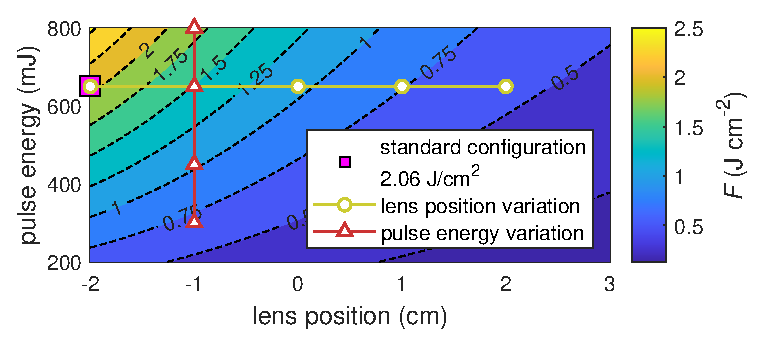
\includegraphics{fluence.eps}
    \caption{Laser energy density depending on the applied pulse energy and lens position. Smaller lens positions yield smaller spot sizes. A value of \qty{-2}{\cm} corresponds to the lens being as close as possible to the laser entrance window in the setup used for this work.
    The default configuration of \qty{650}{\milli\joule} and \qty{-2}{cm} yields typical fluences of about \qty{2}{\J\per\square\cm}.
    The triangles and circles represent the variation of laser fluence in this work, achieved by varying the pulse energy and lens position, respectively.}
    \label{Fig:Methods_fluence}
\end{figure}

\subsection{Plasma Dynamics}
The \gls{pld} procedure can be broken down into three physical processes: (i) energy absorption on the target surface, (ii) formation of a plasma and (iii) condensation on the substrate:
\begin{enumerate}[label=(\roman*)]
    \item After being projected on the surface of the pellet, the radiation penetrates the material only by a fraction of a \unit{\um}.
    Electrons are excited and oscillate in the electromagnetic field of the laser pulse, which is still ongoing.
    Those electrons collide with bulk atoms of the surface region, which are subsequently heated up and vaporize.
    This process is supported by breaking of chemical bonds due to laser radiation.
    \item A material cloud expands perpendicular to the target surface due to Coulomb repulsion and recoil.
    Absorption of remaining laser radiation results in a plasma plume which is narrow for low background partial pressures below \qty{e-4}{\milli\bar}.
    The target is rotated during this process to minimize the deflection of the plasma due to target degradation.
    The kinetic energy of the material in the plasma plume is crucial for the deposition process and can be controlled by background partial pressure and laser energy density on the target.
    \item The plasma plume hits the substrate which results in resputtering of already deposited material, which condensates together with the plasma, resulting in thermal equilibrium and thus thin film nucleation.
    A large number of adatoms results in many nucleation centers which is responsible for smooth films.
\end{enumerate}
It becomes clear, that \gls{pld} is a non-equilibrium process, making empirical optimization of growth parameters an essential part of thin film manufacturing
    \cite{lorenz2019}.

\subsection{Segmented Target Approach}\label{Sec:Methods_VCCS}
To provide a discrete material library -- a set of different samples with homogeneous composition each --, a segmented target approach as described in \textcite{vonwenckstern2020} is applied.
Specifically, the \gls{VCCS} method utilizes a segmented target, i.e.\ a target with distinct regions of different material composition.
By varying the laser spot position on the target, different plasma compositions can be achieved.
Because the target is rotating during \gls{pld}, the material distribution must be in such a way that when the radial position $R$ of the laser on the target changes, the average ablated composition $\chi(R)$ changes.
This can be realized with an elliptical segmentation, i.e.\ a target pellet with overall composition \ce{A_yB_{1-y}}, but containing an inner ellipse with composition \ce{A_xB_{1-x}} (Fig.~\ref{Fig:Methods_pld}b).
By this means, any homogeneous composition \ce{A_$\chi$B_{1-$\chi$}} with $\chi$ between $x$ and $y$ can be realized with only one target.
$\chi$ is related to the path lengths of the moving laser spot on the inner and outer segment, respectively.
The composition in the plasma can be calculated via \cite{vonwenckstern2020}:
\begin{equation}\label{Equ:Methods_composition}
    \chi(R) = y-(y-x)\frac{2}{\pi}\arccos\left[\frac{1}{\delta}\sqrt{1-\left(\frac{b}{R}\right)^2}\,\right]\,
\end{equation}
where $\delta$ and $b$ are eccentricity and semi-minor axis of the ellipse, respectively\footnote{
    The eccentricity is defined as $\delta=\sqrt{1-b^2/a^2}$, where $a$ is the length of the semi-major axis.
}.
Small and large $R$ will result in a composition equal to the composition of the inner and outer segment, respectively.
To model the process more accurately one has to take into account that the laser does not yield a point-like spot but rather an intensity distribution.


\section{X-Ray Diffraction Measurement}
    As described in \ref{Sec:Theory_X-ray_diffraction}, constructive interference of incoming and scattered X-rays may give insight in the symmetry of exposed crystal structures.
This can be utilized for thin film investigation and is called \gls{XRD}.
The \gls{XRD} device used for this work, namely an \textit{X'Pert Pro} (\textit{Malvern Panalytical Ltd.}), as well as the applied scanning techniques will be presented in the following.

A sample with surface normal parallel to the $z$-axis of the laboratory system is exposed with X-rays at an angle $\omega$ between sample surface and incident radiation.
The diffracted radiation is measured at an angle $\alpha_\mathrm{out}$ between sample surface and detector.
$2\theta$ is used to describe the angle between outgoing beam and the extension of the incoming beam, which both span the scattering plane.
It follows that $2\theta=\omega+\alpha_\mathrm{out}$.
Note that $\theta$ in Equ.\,(\ref{Equ:Theory_BraggCondition}) is the same angle as half of $2\theta$.
The scattering plane is depicted in Fig.\,\ref{Fig:Methods_XRD_geometry}a.
The sample can be rotated by $\phi$ (\enquote{azimuth}) and $\psi$ around an axis parallel to the surface normal and parallel to the intersection of sample surface and scattering plane, respectively.

% ---
\subsection{2\texttheta-\textomega-scans}
    \label{Sec:Methods_2ThetaOmega}
% ---
\begin{figure}
    \centering
    \begin{tabular}{ll}
        \textbf{(a)}&\textbf{(b)}\\
        \includegraphics{theta-omega-noTilt.pdf}
        &\includegraphics{theta-omega-Tilt.pdf}
    \end{tabular}
    \caption{\textbf{(a)} Geometry for a 2\texttheta-\textomega-scan without offset.\ \textbf{(b)} Scattering geometry containing an offset $\omega_0$. Angle of incidence and angle of diffraction decrease and increase, respectively. Note that $2\theta$ is not affected by this offset.}
    \label{Fig:Methods_XRD_geometry}
\end{figure}
When probing for lattice plane distances using the \gls{bc} in its simplest form, it is assumed that the scattering planes are parallel to the sample surface (cf. Fig.\,\ref{Fig:Methods_XRD_geometry}a).
It is necessary that $\omega=\alpha_\mathrm{out}$ which implies $2\theta=2\omega$.
So the angle of incidence $\omega$ is coupled to $2\theta$ which represents the distance between lattice planes (cf. Equ.\,(\ref{Equ:Theory_BraggCondition})).
Measuring the diffracted X-ray intensity while varying $2\theta$ and maintaining the condition $2\theta=2\omega$, is called a 2\texttheta-\textomega-scan.
This results in a so-called 2\texttheta-\textomega\ diffraction pattern, where peaks correspond to constructive interference and thus to certain lattice plane distances.

When analyzing 2\texttheta-\textomega\ diffraction patterns, one usually compares to predicted peak positions of the expected phase of the compound which is investigated.
This reference diffraction pattern stems from powder samples of the respective compound, containing all crystal orientations during one 2\texttheta-\textomega-scan.
When a peak is identified, a possible peak shift is determined and the shape of the peak is investigated.
Peak shifts may be due to residual stress, substrate induced strain or compositional gradients in the thin film 
    \cite{harrington2021}.
A minimum amount of peak broadening is always present due to convergence of the incident beam as well as convolution of K\textalpha\textsubscript{1}- and K\textalpha\textsubscript{2}-radiation (cf.~\ref{Sec:Theory_XRays}), which is called instrumental broadening
    \cite{harrington2021}.
The \gls{FWHM} of the highly crystalline substrate peaks may give a reference for broadening of peaks in 2\texttheta-\textomega\ diffraction data.  

This method can be extended to measure lattice planes which are not parallel to the sample surface but tilted by $\omega_0$.
This is done by rotating the reference frame of the sample in such a way that the \gls{bc} is fulfilled again.
Note that $2\theta$ does not change upon rotation, as can be seen in Fig.\,\ref{Fig:Methods_XRD_geometry}b.
When probing for plane distances of the rotated lattice, one finds for the coupling between $2\theta$ and $\omega$:
\begin{align*}
    \omega'&=\alpha_\mathrm{out}'\\
    \omega+\omega_0&=\alpha_\mathrm{out}-\omega_0\\
    \omega+\omega_0&=(2\theta-\omega)-\omega_0\\
    \Rightarrow 2\theta&=2(\omega+\omega_0)=2\omega'\,.
\end{align*}
This coupling is equivalent to a 2\texttheta-\textomega-scan but with an offset $\omega_0$ applied to the angle of incidence.
There are several use cases for applying an offset $\omega_0$:
\begin{enumerate}[label=(\roman*)]
    \item It is assumed that $\omega$ denotes the angle between incident X-ray beam and the sample surface.
    But a perfect alignment between sample and sample holder is not always possible.
    So to correct this tilt between expected sample position and it's real inclination, the offset $\omega_0$ can be set to really probe for lattice planes parallel to the sample surface.
    This is done before measuring a 2\texttheta-\textomega-scan to achieve preciser results.
    \item When probing for lattice planes which are not parallel to the sample surface (\enquote{asymmetric reflections}), one can apply the expected inclination angle as an offset $\omega_0$.
    This is the case in Fig.\,\ref{Fig:Methods_XRD_geometry}b.
    \item When $2\theta$ is fixed, but $\omega_0$ is varied, a so-called \textomega-scan is performed, which enables quantification of mosaicity (cf.~\ref{Sec:Methods_omegaScan}).
\end{enumerate}

% ---
\subsection{\textomega-scans}
    \label{Sec:Methods_omegaScan}
% ---
Thin films may exhibit a distribution of lattice plane inclination, called mosaicity.
This results in an observation of diffraction peaks for several offsets $\omega_0$.
The mosaicity can thus be quantified by fixing $2\theta$, representing a certain lattice plane distance, and then vary $\omega_0$ and measure the X-ray intensity.
This is called an \textomega-scan, and the \gls{FWHM} of the observed diffraction pattern (also called \enquote{Rocking curve}) is a measure for the mosaicity
    \cite{harrington2021}.
\textomega-scans are particularly useful when comparing a set of thin films of varying deposition parameters to optimise growth conditions.
In particular, recording Rocking curves of symmetric and asymmetric lattice planes allows the calculation of dislocation densities in the thin film
    \cite{srikant1997}.
% ---
\subsection{\textphi-scans}
    \label{Sec:Methods_phiScan}
% ---
A 2\texttheta-\textomega-scan is not capable of resolving in-plane rotations of crystal domains, because the distance of lattice planes parallel to the surface are not affected.
Those rotational domains can be detected by probing for lattice planes which are inclined with respect to the surface, i.e.\ by fixing $2\theta$ to the expected lattice plane distance and $\omega_0$ to the inclination angle (cf. Fig.\,\ref{Fig:Methods_XRD_geometry}b).
Depending on the symmetry of the inspected material, constructive interference should only appear for distinct values of $\phi$.
So by rotating the sample by \qty{360}{\degree} and simultaneously recording the X-ray intensity, a so-called \textphi-scan (also called \enquote{Azimuth-scan}) can yield information about the existence of rotational domains.
If the number of observed peaks in the \textphi-scan diffraction pattern exceeds the theoretically expected number for a single crystal, rotational domains are present
    \cite{harrington2021}.
Furthermore, comparing the \textphi-scan diffraction data of thin film and substrate reveals whether the film has grown with an in-plane rotation with respect to the substrate.
Finally, if the thin film grows in a tilted manner on the substrate, a \textphi-scan prior to an \textomega-scan can ensure the correct positioning bevor alignment.
Then, the \gls{bc} is fulfilled for performing a 2\texttheta-\textomega-scan.

% ---
\subsection{Reciprocal Space Maps}
    \label{Sec:Methods_RSM}
% ---
Because the \gls{bc} is equal to the description of diffraction with $\mathbf{k}'-\mathbf{k}$ and reciprocal space vectors $\mathbf{K}_{hkl}$ (cf.~\ref{Sec:Theory_X-ray_diffraction}), both can be used depending on context.
Henceforth, $\mathbf{k}'-\mathbf{k}$ will be denoted by the \enquote{scattering vector} $\mathbf{q}$.
Note that $\mathbf{k}$ and $\mathbf{k}'$ are parallel to incoming and outcoming beam, respectively.
From the definition of angles, it follows that
\begin{align}
    \mathbf{q}
    =\begin{pmatrix}
        q_\parallel\\
        q_\perp
    \end{pmatrix}
    &=\mathbf{k}'-\mathbf{k}\\
    &=\frac{1}{\lambda}
    \begin{pmatrix}
        \cos\alpha_\mathrm{out}\\
        \sin\alpha_\mathrm{out}
    \end{pmatrix}
    -\frac{1}{\lambda}
    \begin{pmatrix}
        \cos\omega\\
        -\sin\omega
    \end{pmatrix}\\
    &=\frac{1}{\lambda}
    \begin{pmatrix}
        \cos(2\theta-\omega)-\cos(\omega)\\
        \sin(2\theta-\omega)+\sin(\omega)
    \end{pmatrix}\,.
    \label{Equ:Methods_qDef}
\end{align}
From Equ.\,(\ref{Equ:Methods_qDef}), two properties follow for the scattering vector:
\begin{align}
    -q_\parallel/q_\perp&=-\tan\left(\omega-\frac{2\theta}{2}\right)=\tan\omega_0
        \label{Equ:Methods_qDir}\,,\\
    \left|\mathbf{q}\right|&=\sqrt{q_\parallel^2+q_\perp^2}=\frac{1}{\lambda}2\sin\theta\overset{\mathrm{Bragg}}{=}\frac{1}{d_{hkl}}\,,
    \label{Equ:Methods_qAbs}
\end{align}
where the last equality of Equ.\,(\ref{Equ:Methods_qAbs}) holds, if $\mathbf{q}$ is a reciprocal lattice vector $\mathbf{K}_{hkl}$.
The scattering vector, together with the corresponding \gls{XRD} geometry is depicted in Fig.\,\ref{Fig:Methods_qDef}a.
\begin{figure}
    \centering
    \begin{tabular}{ll}
        \textbf{(a)}&\textbf{(b)}\\
        \includegraphics{reciprocalDef.pdf}
        &\includegraphics{correctReciprocal.pdf}
    \end{tabular}
    \caption{\textbf{(a)} Construction of the scattering vector (magenta) from incoming (red) and outgoing (green) beam, according to Equ.\,(\ref{Equ:Methods_qDef}).
    The reciprocal lattice points are visualized together with the lattice planes.
    It has to be noted that the distances between lattice planes and between reciprocal lattice points have different dimensions.\ 
    \textbf{(b)}\tbd}
    \label{Fig:Methods_qDef}
\end{figure} 
Because $2\theta$ and $\omega$ can simultaneously be represented by $\mathbf{q}$, it is possible to measure intensities for several $\mathbf{q}$, such that a part of the reciprocal space $Q\ni\mathbf{q}$ is mapped.
Consequently, this is called a \gls{RSM}.
According to Equ.\,(\ref{Equ:Theory_ConstructiveInterference}), a peak in 2D reciprocal space $Q$ should be observed if $\mathbf{q}$ is a reciprocal space vector.
In this case, $\mathbf{q}=\mathbf{K}_{hkl}$ is called a \enquote{reflection}.
With Equ.\,(\ref{Equ:Methods_qDir}) one can determine $\omega_0$ -- the direction of the corresponding lattice planes\footnote{
    Note that the \enquote{$-$} in $-q_\parallel/q_\perp$ is necessary, such that this fraction is the tangens the angle between $\mathbf{q}$ and surface normal with correct sense of rotation. 
}, and with Equ.\,(\ref{Equ:Methods_qAbs}) the lattice plane distance $d_{hkl}$ can be calculated.
Note that for rhombohedral crystals, $d_{hkl}$ can also be predicted from the lattice constants $a$ and $c$ with the following equation \cite{grundmann2018}:
\begin{equation}
    d_{hkl}=\left(
        \frac{4}{3}\frac{h^2+k^2+hk}{a^2}
        +\frac{l^2}{c^2}
    \right)^{-1/2}\,.
    \label{Equ:Methods_dhkl}
\end{equation}
The inclination with respect to the \textit{c}-axis can be determined via \cite{grundmann2020b}
\begin{equation}
    \alpha_{hkl|c}
    \arccos\left(
        \frac{l}{\sqrt{
            \frac{4c^2}{3}\frac{h^2+k^2+hk}{a^2}+l^2
        }}
    \right)\,.
    \label{Equ:Methods_angleWRTc}
\end{equation}


A 2\texttheta-\textomega-scan corresponds to a set of $\mathbf{q}$ with fixed direction in reciprocal space, but varying length.
For scanning symmetric reflections, $\mathbf{q}$ is parallel to the surface normal (as in Fig.\,\ref{Fig:Methods_qDef}a).
On the other hand, an \textomega-scan corresponds to a set $\mathbf{q}$ with fixed length but varying direction.
The mosaicity can therefore approximately quantified by the broadening of a reflection perpendicular to the direction of $\mathbf{K}_{hkl}$.
Because anisotropic strain has an effect on direction and length of inclined lattice planes, asymmetric reflections, i.e.\ $\omega_0\neq0$, can be deconvoluted into an in-plane and out-of-plane component.
By this means, \glspl{RSM} enable the calculation of lattice constants.
To precisely calculate the latter, several corrections are applied to the recorded \glspl{RSM}, as proposed in \textcite{kneiss2021}:
\begin{enumerate}
    \item High-quality sapphire substrates are used for deposition of thin films.
    It can be assumed that they have the expected crystal structure of bulk \textalpha-\ce{Al2O3} (cf. Tab.\,\ref{Tab:sesquiLatticeConstants}).
    So any deviation of the observed reflection $\mathbf{q}_{hkl}^\mathrm{\ce{Al2O3},obs}$ from the expected peak position $\mathbf{q}_{hkl}^\mathrm{\ce{Al2O3},lit}$ is corrected by a rotation $\mathbf{R}$ and scaling $\rho$ of reciprocal space $Q$:
    \begin{equation}
        \mathbf{q}^\mathrm{cor}=\rho\mathbf{R}\cdot\mathbf{q}^\mathrm{obs}\quad,\quad\mathbf{q}^\mathrm{obs}\in Q\,,
    \end{equation}
    with
    \begin{align}
        \label{Equ:Methods_rotation}
        \mathbf{R}&=\begin{pmatrix}
            \cos\gamma&-\sin\gamma\,,\\
            \sin\gamma&\cos\gamma
        \end{pmatrix}\quad,\quad
        \gamma=\arccos\left(
            \frac
                {\mathbf{q}_{hkl}^\mathrm{\ce{Al2O3},lit}
                    \cdot\mathbf{q}_{hkl}^\mathrm{\ce{Al2O3},obs}}
                {\left|\mathbf{q}_{hkl}^\mathrm{\ce{Al2O3},lit}\right|
                    \cdot\left|\mathbf{q}_{hkl}^\mathrm{\ce{Al2O3},obs}\right|}
            \right)\\
        \rho&=\frac{\left|\mathbf{q}_{hkl}^\mathrm{\ce{Al2O3},lit}\right|}{\left|\mathbf{q}_{hkl}^\mathrm{\ce{Al2O3},obs}\right|}\,.
    \end{align}

    \item If the thin film grows tilted (e.g.\ due to slip systems, cf.~\ref{Sec:Theory_Relaxed}), a symmetric reflection -- having scattering vector parallel to the surface normal in theory -- will exhibit an in-plane component $q_{\parallel,hkl}^\mathrm{film}\neq0$.
    The tilt angle can be calculated by Equ.\,(\ref{Equ:Methods_qDir}): 
    \begin{equation}
        \theta_\mathrm{tilt}=\arctan\left(-\frac{q_{\parallel,hkl}^\mathrm{film}}{q_{\perp,hkl}^\mathrm{film}}\right)\,.
    \end{equation}
    To determine the lattice constants from asymmetric peaks, the reciprocal space is again rotated as in Equ.\,(\ref{Equ:Methods_rotation}) but with rotation angle $-\theta_\mathrm{tilt}$.
    This scenario is depicted in Fig.\,\ref{Fig:Methods_qDef}b, where the magenta colored reflection deviates from the expected symmetric position.

    \item If the thin film is sheared, a symmetric reflection $\mathbf{q}_{\tilde{h}\tilde{k}\tilde{l}}^\mathrm{film}$ will be unaffected.
    On the contrary, an asymmetric reflection with both in- and out-of-plane component is affected.
    To get reliable results for the lattice constants, this shear angle $\Psi_\mathrm{shear}$ has also to be corrected, and can be calculated from two inclined lattice planes ($hkl$) and ($h'k'l'$), i.e.\ scattering vectors with non-zero in-plane component.
    Those vectors must have symmetry of a mirror plane perpendicular to the scattering plane\footnote{
        This can be achieved by probing for a plane ($hkl$) and then rotate the sample around $\phi$ by \qty{180}{\degree}.
    }.
    The geometry is depicted in Fig.\,\ref{Fig:Methods_qDef}b, with the blue and green reflections representing the symmetric and asymmetric reflections, respectively.
    The shear angle can be calculated with
    \begin{equation}
        \Psi_\mathrm{shear}=\arctan\left(\frac{
            q_{\perp,hkl}^\mathrm{film}
            -q_{\perp,h'k'l'}^\mathrm{film}
        }{
            q_{\parallel,hkl}^\mathrm{film}
            -q_{\parallel,h'k'l'}^\mathrm{film}
        }\right)\,.
        \label{Equ:Methods_shearAngle}
    \end{equation}
    To correct the shear, a rotation around the corresponding symmetric reciprocal lattice point $\mathbf{q}_{\tilde{h}\tilde{k}\tilde{l}}^\mathrm{film}$ with the same expected out-of-plane component must be applied.
\end{enumerate}

\subsection{Technical Aspects}
The radiation is produced by an copper anode, resulting in a wavelength of $\lambda=\qty{1.5406}{\angstrom}$ for \ce{Cu}-K\textalpha\textsubscript{1} radiation.
Note that \ce{Cu}-K\textalpha\textsubscript{2} and \ce{Cu}-K\textbeta\ radiation is not filtered out, resulting in additional low-intensity peaks in the diffractograms.
Furthermore, contamination of the anode with tungsten results in an observable \ce{W}-L\textalpha\textsubscript{1} contribution with energy between \ce{Cu}-K\textalpha- and \ce{Cu}-K\textbeta-radiation.
During the course of the conducted experiments, the contaminated anode has been replaced, so the peaks corresponding to \ce{W}-L\textalpha\textsubscript{1}-radiation are not present in every diffractogram.

The diffracted radiation is detected with a \textit{PIXcel\textsuperscript{3D}} (\textit{Malvern Panalytical Ltd.}) detector.
For 2\texttheta-\textomega-scans (cf.~\ref{Sec:Methods_2ThetaOmega}), the detecor is operating in \enquote{Scanning Line} mode.
For scans fixing the 2\texttheta\ position, i.e.\ \textomega- (cf.~\ref{Sec:Methods_omegaScan}) and \textphi-scans (cf.~\ref{Sec:Methods_phiScan}), the detector is operated in \enquote{Receiving Slit} mode.
\glspl{RSM} are recorded with the \enquote{Frame Based} mode.
The settings for the various scans are listed in Tab.\,\ref{Tab:Methods_XRDSettings}.
Note that it is distinguished between scans and optimizations.
The latter were applied for aligning the sample correctly, depending on the measurement.
For example, before a 2\texttheta-\textomega-scan of \textit{m}-plane oriented rhombohedral samples, a \textphi-scan has been applied for the inclined (30.6) reflection to find the correct azimuth of the \textit{c}-axis, which is called \textphi-optimization.
Afterwards, a Rocking curve has been recorded and $\omega$ set to the maximum of the peak to compensate for the expected lattice tilt (cf.\,\ref{Sec:Theory_Relaxed}), called an \textomega-optimization.

\begin{table}
    \centering
    \caption{Configurations for the applied \gls{XRD} scans.}
    \label{Tab:Methods_XRDSettings}
    \begin{tabular}{cllll}
        \toprule
        scan type
            & detector mode
            & step size (\unit{\degree})
            & active channels
            & effective width \\
        \midrule
        2\texttheta-\textomega-scan
            & 1D Scanning Line
            & 0.005
            & 255
            & \qty{2.51}{\degree} \\
        \cmidrule{1-2}
        \textomega-scan
            & 0D Receiving Slit
            & 0.005
            & 55
            & \qty{3.025}{\mm} \\
        \textomega-optimization
            & 0D Receiving Slit
            & 0.02
            & 37
            & \qty{2.035}{\mm} \\
        \cmidrule{1-2}
        \textphi-scan 
            & 0D Receiving Slit
            & 0.05
            & 55
            & \qty{3.025}{\mm} \\
        \textphi-optimization
            & 0D Receiving Slit
            & 0.5
            & 55
            & \qty{3.025}{\mm} \\
        \cmidrule{1-2}
        RSMs
            & 1D Frame Based
            & 0.005
            & 255
            & \qty{2.51}{\degree} \\
        \bottomrule
    \end{tabular}
\end{table}


\section{Thermal Evaporation}
    The ohmic contacts for electrical characterization of \ce{Cr2O3} thin films were deposited by means of thermal evaporation.
This method was already utilized for successfully contacting \agao\ thin films
    \cite{vogt2023},
thus also applied for similarly structured \cro\ thin films.
This \gls{pvd} method utilizes a \emph{boat} made of a material with high melting temperature (tungsten \ce{W} or molybdenum \ce{Mo}) that is loaded with the target material in form of powder or filament.
A vacuum chamber is used to achieve pressures of around \qty{5e-5}{\milli\bar}.
A high current is driven through the contacted boat, such that resistive heating ensures melting of the target material and subsequent evaporation.
The evaporated material spreads out due to the pressure gradient and condensates on the sample which is mounted to a rotating holder.
A metal mask ensures that only the corners of the sample are contacted.

The contacts are either a stacking of titanium, aluminum, and gold (henceforth referred to as \emph{Ti-Al-Au}) or only titanium and gold (\emph{Ti-Au}).
The thickness of each material layer is around \qty{30}{\nm}, measured with a crystal oscillator during the process.
The currents used for evaporating \ce{Ti}, \ce{Al} and \ce{Au} are \qty{60}{\ampere}, \qty{50}{\ampere} and \qty{45}{\ampere}, respectively.
\section{Resistivity Measurement}
    \begin{figure}
    \centering
    \includegraphics[align=c]{vanDerPauw.pdf}
    \caption{The geometry for measuring the specific resistance of a thin film, proposed by \textcite{pauw1958}.}
    \label{Fig:Methods_pauwGeometry}
\end{figure}

As shown by \textcite{pauw1958}, it is possible to determine the specific resistivity of a flat sample by only making four small contacts at arbitrary points at its edge and measure the thickness $t$ as well as the following resistances\footnote{
    The unit of those quantities is \unit{\ohm}, thus the name.
}:
\begin{equation}
    R_{AB,CD}=\frac{V_D-V_C}{I_{AB}}\quad , \quad
    R_{BC,DA}=\frac{V_A-V_D}{I_{BC}}\,,
\end{equation}
where $V_D-V_C$ is the potential difference between points $C$ and $D$, measured while applying $I_{AB}$, the current entering the sample at point $A$ and leaving it at point $B$.
The geometry\footnote{
    Note that \eqref{Equ:Methods_pauw} is restricted to these conditions:
    \textquote[\textcite{pauw1958}]{%
        (a) The contacts are at the circumference of the sample. (b) The contacts are sufficiently small. (c) The sample is homogeneous in thickness. (d) The surface of the sample is singly connected, i.e., the sample does not have isolated holes.%
        }
} is depicted in Fig.\,\ref{Fig:Methods_pauwGeometry}a.
The specific resistivity $\rho$ can then be calculated via
\begin{equation}
    \label{Equ:Methods_pauw}
    \rho=
    \frac{\pi t}{\ln2}
    \frac{R_{AB,CD}+R_{BC,DA}}{2}
    \cdot f\left(\frac{R_{AB,CD}}{R_{BC,DA}}\right)\,,
\end{equation}
where $f$ is a function equal to 1, if the two measured resistances are equal; $f$ decreases for higher ratios of the two measured resistances
    \cite{pauw1958}.
The geometry can further be used to determine the Hall mobility $\mu_H$ and carrier concentration $n$, but due to low conductivities of the here investigated \cro\ thin films, this method yields no reliable information about $\mu_H$ and $n$.

Temperature-dependent resistivity measurements are conducted with a Hall probe station \textit{CRX-VF} controlled by the measurement setup \textit{HM-8425} (Lake Shore Cryotronics, Inc.), cooled via a \textit{Model 336 cryogenic temperature controller} (Lake Shore).
The samples are measured in a vacuum and the temperature can be controlled between \qty{10}{\kelvin} and \qty{390}{\kelvin}.
        \label{Sec:Methods_vanDerPauw}
\section{Thickness Determination}
    spectroscopic ellipsometry is a method to measure the optical constants and thickness $t$ of a thin film by the change of polarization state upon light reflection.
If the probing light covers several wavelengths at once, one refers to spectroscopic ellipsometry, which will be presented in the following, based on \textcite{fujiwara2007}.
The incoming light can be represented by an electromagnetic wave, decomposed into two components being parallel (p) and perpendicular (s) to the scattering plane:
\begin{equation}
    \mathcal{E} = \mathcal{E}_\mathrm{ip} + \mathcal{E}_\mathrm{is}\,.
\end{equation}
In general, the amplitudes of p- and s-polarized light change in a different manner after reflection, so the overall polarization of the reflected light is changed.
This change is described by the fraction
\begin{equation}
    \rho=\frac{r_\mathrm{p}}{r_\mathrm{s}}:=\tan\Psi\cdot\exp(i\Delta)\,,
\end{equation}
where $r_\mathrm{p}$ and $r_\mathrm{s}$ are the amplitude reflection coefficients\footnote{
    They are defined by the amplitude of incoming (i) and reflected (r) radiation: $r=|\mathcal{E}_\mathrm{r}|/|\mathcal{E}_\mathrm{i}|$.
} for the p- and s-polarized component, respectively.
For simple structures, $\Psi$ is essentially the refractive index $n$, and $\Delta$ represents the extinction coefficient $k$.
In general, they can be calculated from the \textsc{Jones}-matrix -- representing the reflection -- and depend on the angle of incidence as well as the photon energy.

To determine the sample thickness, the spectra of $\Psi$ and $\Delta$ can be generated using a model for the sample structure, which is then fitted to the experimental data.
In this work, this model consists of an \ce{Al2O3} substrate without backscattering from the backside (infinite thickness); a \cro\ thin film of thickness $t$; and a mixed layer of air and \cro, approximating the roughness of the sample.
Because the measured spectra were confined to the visible regime of the thin film (approx. $<\qty{2.8}{\eV}$), one can apply the \textsc{Cauchy} model
    \cite{fujiwara2007},
approximating the refractive index by
\begin{equation}
    n(\lambda)=A+\frac{B}{\lambda^2}+\frac{C}{\lambda^4}+\mathcal{O}\left(\lambda^{-6}\right)\quad,\quad k=0\,.
\end{equation}

The spectroscopic ellipsometry measurements were performed with an \textit{M-2000VI} (J.A.\ Woolam Co., Inc.) and the data was analyzed using the software \textit{WVASE} (J.A.\ Woolam).
The angles of incidence were chosen to be \qty{50}{\degree}, \qty{60}{\degree} and \qty{70}{\degree}, and the modelled spectral range is \qtyrange{0.75}{2.8}{\eV}.
If samples of different orientation were fabricated in the same process, one can assume similar thicknesses, and a measurement with three angles was conducted only for one sample of the batch.
The other samples were measured with only one angle, if the determined thickness did not differ significantly from the more accurately measured one.

Note that the investigated thin films are not isotropic in general, which is why the validity of the determined thickness is checked by profilometer measurements with a \textit{Dektak XT Stylus Profiler} (Bruker Corporation).
The edges of the quadratic substrates are masked by the sample holder during deposition, which is why they are not deposited with the target material.
Consequently, measuring the height profile ranging from an edge to coated regions of the sample yields an approximation for $t$ by the height of the observed step edge.


\section{Spectral Transmission}
    For optical characterization, spectral transmission measurements were conducted:
Mo\-no\-chro\-ma\-tic light is used to compare a reference beam with the intensity of radiation transmitting a sample of thickness $t$.
The fraction of both is defined as the transmittance $T(E)$ which depends on the photon energy $E=\hbar\omega$.
In a simple model, neglecting reflection on the sample surface as well as thin film interference
    \cite{manifacier1977},
the absorption coefficient $\alpha$ can be defined via the \textsc{Lambert}-\textsc{Beer}-law:
\begin{equation}
    T\propto e^{-\alpha t}\,,
\end{equation}
which states an exponential decay of intensity with increasing thickness $t$.
The absorption coefficient is based on the transition rate between valence band and conduction band at photon energy $E$.
This rate depends on the energy-dependent coupling matrix element for this transition, as well as the joint electron and hole \gls{DOS}
    \cite{zanatta2019}.
If matrix element and \gls{DOS} are assumed to be constant and parabolic, respectively
    \cite{tauc2005},
then $\alpha=0$ for energies below the band gap, and for direct transitions it follows \cite{zanatta2019}:
\begin{equation}
    \alpha\propto (E-E_g)^{1/2}\,.
\end{equation}
This allows extrapoliting an $\alpha^2$ vs.\ $E$ plot to the abscissa to determine the band gap $E_g$.
For indirect transitions, phonons with energy $\hbar\Omega$ must be considered which leads to
\begin{equation}
    \alpha\propto (E+\hbar\Omega-E_g)^2\,,
\end{equation}
which itself allows the determination of the band gap by extrapoliting an $\alpha^{1/2}$ vs.\ $E$ plot, if the phonon energy is neglected
    \cite{zanatta2019}.
According to \textcite{zanatta2019}, these two methods are often mislabeled as \textsc{Tauc} plots $\alpha^\eta$ vs.\ $E$ with exponent $\eta$ defining the direct or indirect nature of the transition.
Actually, those methods are based on the description of \emph{crystalline} solids, whereas the original \enquote{\textsc{Tauc} plot} was an empirical description of \emph{amorphous} germanium, leading to an $(\alpha E)^{1/2}$ vs.\ $E$ plot
    \cite{tauc2005}.
This method has been applied
    \cite{cheng1996,al-kuhaili2007,singh2019,farrell2015},
to determine the band gap of crystalline solids, which is an inappropriate use of the \textsc{Tauc} method, which can be only applied if localized energy states are present, as in amorphous solids or nanoparticles
    \cite{dolgonos2016}.
In this work, a direct band gap of \cro\ is assumed and therefore the $\alpha^2$ vs.\ $E$ plot is utilized.
This is described in more detail in~\ref{Sec:Results_Preliminary}.

In general, it has to be noted that the value obtained from extrapolating any of those plots to the abscissa is affected by several approximations:
    no \textsc{Coulomb} interaction between holes and electrons is considered;
    defect states that could enable absorption below $E_g$ are neglected;
    the parabolic nature of the \gls{DOS} is only true for $k\approx0$ and not for large energies $\hbar\omega\gg E_g$;
    differences in selecting the regime that is selected for fitting may result in substantial deviations for the values of $E_g$
    \cite{zanatta2019}.
Due to those considerations, the value extrapolated from $\alpha^2$ vs.\ $E$ plots will be called optical gap $E_\mathrm{opt}$.
Due to the fact that the intersection of 
\begin{equation*}
    \alpha=\mathrm{const.}\cdot(E-E_\mathrm{opt})^{1/2}
\end{equation*}
with the abscissa does not depend on the value of $\mathrm{const.}$, the $\alpha^2$ vs.\ $E$ plots are visualized with arbitrary units on the ordinate (cf.\ Fig.\,\ref{Fig:Results_1_transmission}b or Fig.\,\ref{Fig:Results_3_lensTransmission}).

%! experiment
The measurements were conducted in a spectral range of \qtyrange{200}{2800}{\nm}, realized by two light sources with a \textit{Lambda 40} (Perkin-Elmer).
The spectra are corrected with a corresponding reference substrate.
The measurements were done by M.\ Hahn.
        \label{Sec:Methods_transmission}
\section{Further Measurement Methods}
    \acrfull{AFM} is a method to measure the force between a probe and the sample, which itself depends on several factors, including the distance between probe and sample.
By scanning a cantilever with a sharp tip over the sample, it is possible to yield a topological map of the surface
    \cite{schroder2005}.
The measurements were kindly performed by M.\ Sc.\ C.\ Dethloff.

\acrfull{RHEED} is a method to probe the crystal structure of only a few monolayers below the surface of a thin film.
High-energy electrons are pointed in grazing incidence geometry on the sample surface and the diffracted electrons are detected with a fluoroescent screen.
The image of the screen is called the RHEED pattern and it can yield information about the symmetry and crystallinity of the sample surface
    \cite{hafez2022}.

\acrfull{TEM} is a method for providing highly magnified images of solid state samples.
The method utilizes a beam of high energy electrons that is passing through a sufficiently thin sample.
Resolutions of \qty{0.08}{\nm} can be achieved due to the shorter wavelength of electrons compared to visible light
    \cite{schroder2005}.
A scanning \acrshort{TEM} method is \gls{HAADF}, where scattered electrons are detected with an annular dark field detector.
The \acrshort{HAADF} images in this work were kindly performed by Dr.\ J.\ G.\  Fernandez.
        \cleardoublepage
    \chapter{Experiment, Results and Discussion}
\minitoc
%! (1)
    \section{Preliminary Investigations}
    \label{Sec:Results_Preliminary}
%! Motivation / Intro
In the following, the feasibility of depositing \cro\ thin films via \gls{pld} as well as their resulting physical properties are investigated.
Because \cro\ is the most stable chromium oxide, its formation is expected, but other oxidation states cannot be excluded.
E.g., in Fig.\,\ref{Fig:Results_2_photoTarget}, a silver colored target coating can be observed, presumably corresponding to metallic \ce{CrO2}.
If \cro\ is the only oxidation state, then amorphous or rhombohedral films are expected, because no other polymorph of \cro\ exists.
Furthermore, if a crystalline phase is present, the orientation with respect to the sapphire substrates is of interest.
Because \alo\ and \cro\ exhibit the same crystal symmetry, it is expected that the crystal orientation of the film  matches the corresponding substrate orientation.
Finally, deposition parameters should be optimized to obtain the best crystal quality.

\subsection{Experiment}
    Due to the similar crystal structure of \cro\ and \agao, the deposition parameters of the latter were chosen as a starting point to deposit chromia thin films on $10\times\qty{10}{\mm\squared}$ sapphire substrates with \textit{m}-plane orientation
    \cite{petersen2023}.
Namely, a pulse energy of \qty{650}{mJ} and a pulse frequency of \qty{20}{\Hz} were applied for a total of \qty{30000} pulses.
To investigate the influence of deposition parameters, three batches were produced:
\begin{enumerate}
    \item variation of oxygen partial pressure $p(\ce{O2})$ from \qtyrange{8e-5}{1e-2}{mbar} with a fixed temperature of \qty{745}{\degreeCelsius},
    \item variation of growth temperature from \qtyrange{725}{765}{\degreeCelsius} with a fixed oxygen partial pressure of \qty{1e-3}{mbar}, and
    \item variation of substrate orientation between \textit{c}- (00.1), \textit{r}- (01.2) \textit{m}- (10.0) and \textit{a}-plane (11.0) $5\times\qty{5}{\mm\squared}$ sapphire substrates\footnote{
        In the following, the \textsc{Bravais}-\textsc{Miller}-indices will be omitted.
        }
    with a fixed oxygen partial pressure of \qty{1e-3}{mbar} and a growth temperature of \qty{715}{\degreeCelsius}.
\end{enumerate}
Structural properties of those thin films were determined by \thetaomega-scans, \textomega-scans and \textphi-scans.
The thickness was determined via spectroscopic ellipsometry, and transmission spectra were recorded for two samples of the 1st batch to determine the optical band gap.
By dividing the thickness by the number of applied pulses, the growth rate $g$ can be calculated as is provided in units of \unit{\pm\per\pulse}.
Temperature dependent resistivity measurements were performed only for the samples of the 3rd batch, because all \textit{m}-plane oriented samples showed no conductivity at room temperature.

\begin{figure}
    \centering
    \includegraphics{camera_initial}
    \caption{
        Image of the samples produced at different oxygen partial pressures ($T=\qty{740}{\degreeCelsius}$) and different growth temperatures ($p(\mathrm{O_2})=\qty{1e-3}{\milli\bar}$).
    }
    \label{Fig:Results_1_samplesPhoto}
\end{figure}

\subsection{Results}
    \subsubsection{Oxygen Partial Pressure Variation on \textit{m}-plane Sapphire}
        %! 2theta-omega scans
\begin{figure}
    \centering
    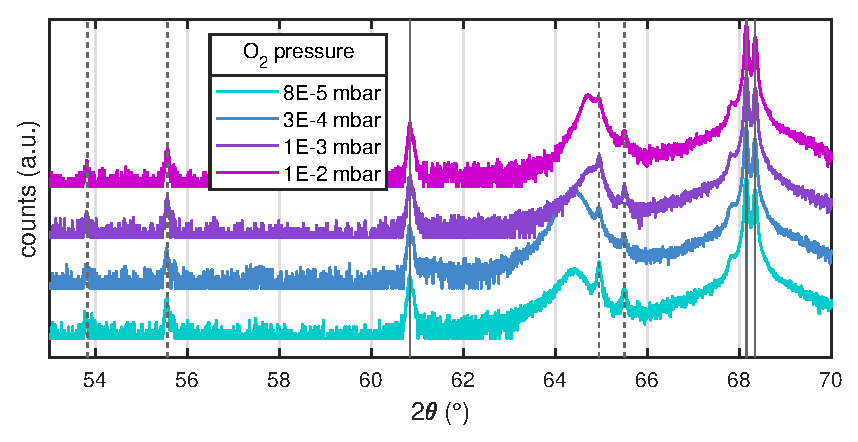
\includegraphics{1_pressure_2theta.eps}
    \caption{\thetaomega-patterns of \cro\ thin films deposited on \textit{m}-plane sapphire for various oxygen partial pressures.
    The solid lines indicate (30.0) substrate reflections corresponding to copper radiation, whereas the dashed lines indicate (30.0) substrate reflections corresponding to tungsten radiation.}
    \label{Fig:Results_1_pressure_2theta}
\end{figure}
In the following, the results for the samples produced at four different oxygen partial pressures are analyzed.
In Fig.\,\ref{Fig:Results_1_pressure_2theta}, the \thetaomega-patterns are depicted.
For each pattern, the two peaks (solid line) at around \qty{68}{\degree} correspond to the (30.0) reflection of the \textit{m}-plane oriented sapphire substrate.
The splitting occurs due to the similar wavelength of \ce{Cu}-K\textalpha\textsubscript{1} and \ce{Cu}-K\textalpha\textsubscript{2} radiation.
The additional peaks also stem mainly from the (30.0) reflection of \ce{Al2O3} and are caused by
\ce{W}-L\textbeta\textsubscript{2}-,
\ce{W}-L\textbeta\textsubscript{1}-,
\ce{Cu}-K\textbeta-,
\ce{W}-L\textalpha\textsubscript{1}- and
\ce{W}-L\textalpha\textsubscript{2}-radiation (increasing angles).\footnote{
    %TODO
    \bfseries\textcolor{red}{Klar wäre das besser das im plot an die linien zu schreiben, aber das war mir irgendwie zu auffändig es schön zu machen. Gehts auch so?}
}
In the vicinity of the calculated peak position for the (30.0) reflection of \cro\ (cf.~\ref{tab:d_strained}), there is a peak observed for each sample, indicating that the \textalpha-phase of \cro\ is present.
Note that the peak position is varying depending on the chosen oxygen partial pressure.
The difference to the expected peak position $2\theta_0$ is expressed as \gls{oop}\ strain $\epsilon_{zz}$ using the Bragg equation Equ.\,\ref{Equ:Theory_BraggCondition} and then
\begin{equation}
    \label{Equ:Results_oop_strain_def}
    \epsilon_{zz}
    =\frac{d-d_0}{d_0}
    =\left(\frac{1}{\sin(2\theta/2)}-\frac{1}{\sin(2\theta_0/2)}\right)
    \cdot\sin(2\theta_0/2)\,.
\end{equation}
In Fig.\,\ref{Fig:Results_1_both_strainFWHM}a, the calculated strain is shown in dependence of the corresponding oxygen partial pressure.
The strain decreases from approx.\ \qty{0.95}{\percent} to \qty{0.45}{\percent} with increasing pressure.
This strain reduction may therefore be the result of increased background gas scattering which results in less kinetic energy of the specimen reaching the heated substrate (cf.~\ref{Sec:Methods_pld}).
\begin{figure}
    \centering
    \begin{tabular}{ll}
        \textbf{(a)}&\textbf{(b)} \figSpace\\
        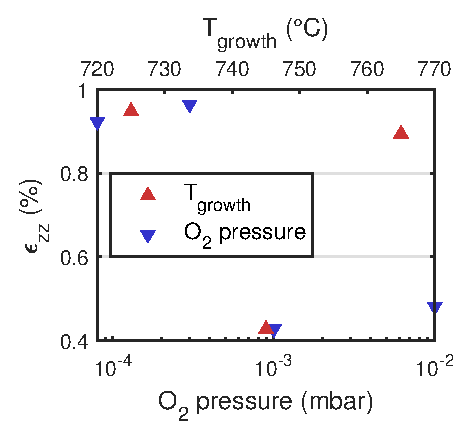
\includegraphics[align=c]{1_both_strain.eps}    
        &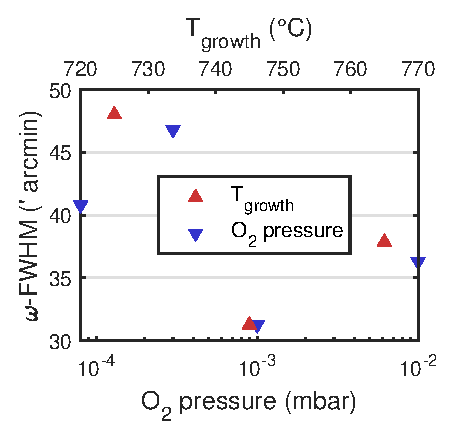
\includegraphics[align=c]{1_both_FWHM.eps}
    \end{tabular}
    \caption{
        \textbf{(a)} \gls{oop}\ strain calculated with Equ.\,\ref{Equ:Results_oop_strain_def} and \textbf{(b)} \textomega-FWHMs for samples from growth temperature series (red triangles, top \textit{x}-axis) and oxygen partial pressure series (blue triangles, bottom \textit{x}-axis).
        }
    \label{Fig:Results_1_both_strainFWHM}
\end{figure}

%! omega-scans
For each sample, the $2\theta$ angle was fixed to the observed (30.0) reflection of \cro\ and an \textomega-scan was performed.
The \glspl{FWHM} of the \textomega-patterns (henceforth \enquote{\textomega-FWHM}) are depicted in
    Fig.\,\ref{Fig:Results_1_both_strainFWHM}b.
The values vary between approx.\ \qtylist{30;50}{\arcminute} and show a dependence on oxygen partial pressure, which is less pronounced compared with \gls{oop}\ strain
    (Fig.\,\ref{Fig:Results_1_both_strainFWHM}a).
Still, since \textomega-FWHM is connected to the mosaicity of the thin film, higher oxygen partial pressures yield slightly better crystal qualities.
Note that due to the fact that an oxygen partial pressure of \qty{1e-3}{\milli\bar} yielded the best crystal quality, this value is used for future deposition processes.

%! phi-scan
To probe for rotational domains of the thin films, \textphi-scans were performed by fixing $2\theta$ and $\omega$ to the corresponding angles of the (30.6) plane of \cro, which has an inclination angle of \qty{32.4}{\degree} with respect to the (30.0) plane.
The diffraction patterns are depicted in Fig.\,\ref{Fig:Results_1_phiScan}.
The observed peaks of the thin film align with the peaks of the single crystal substrate, indicating that the film has no in-plane rotation with respect to the substrate.
Furthermore, the absence of additional peaks indicates that there exists only a single domain of the thin film.
\begin{figure}
    \centering
    \includegraphics{1_both_phi.eps}
    \caption{Diffraction patterns of \textphi-scans performed on the inclined (30.6) reflections for \textit{m}-plane \cro\ (darker color) and \ce{Al2O3} (brighter color).
    The diffraction patterns cover the samples from variation of oxygen partial pressure (teal to blue colored) and variation of growth temperature (red to yellow colored).
    }
    \label{Fig:Results_1_phiScan}
\end{figure}

%! growth rates
The growth rate $g$ varies between \qtylist{3;7}{\pm\per\pulse} and is depicted in Fig.\,\ref{Fig:Results_1_growthRates_photograph}a.
No systematic dependence on the oxygen partial pressure can be observed.
\begin{figure}
    \centering
    \begin{tabular}{ll}
        \textbf{(a)} & \textbf{(b)} \figSpace\\
        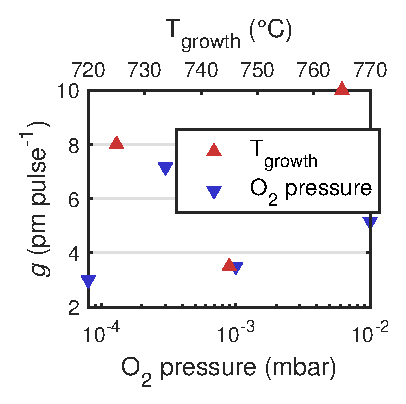
\includegraphics[align=c]{1_both_growthrate.eps}
        &\includegraphics[align=c]{camera_initial.eps}
    \end{tabular}
    \caption{
        \textbf{(a)} Growth rates $g$ for samples from growth temperature series (red triangles, top \textit{x}-axis) and oxygen partial pressure series (blue triangles, bottom \textit{x}-axis).
        \textbf{(b)} Image of the samples produced at different oxygen partial pressures and different growth temperatures.
        }
    \label{Fig:Results_1_growthRates_photograph}
\end{figure}

%! Transmission
The transmission spectra of two selected \cro\ thin films are shown in Fig.\,\ref{Fig:Results_1_transmission}a.
The samples are not fully transparent in the visible spectrum and they exhibit a greenish tint, as can also be seen in Fig.\,\ref{Fig:Results_1_growthRates_photograph}b.
% fitting with indirect gap: cheng 1996, al-kuhaili2007 (^1/2)
% fitting with direct gap: farrell 2015 (^2)
% mi2018 states cr2o3 is a direct bandgap semiconductor
To determine the onset of absorption $E_\tau$, a \textsc{Tauc}-plot (Fig.\,\ref{Fig:Results_1_transmission}b) is utilized (cf.~\ref{Sec:Methods_transmission}).
The exponent is chosen to be $\frac{1}{2}$, resulting in a representation of $(\alpha E)^2$ vs.\ $E$.
Although the publications used for reference in this work support the direct transition nature of \cro\ 
    \cite{farrell2015,mi2018},
it has to be noted that there exist studies determining the optical band gap of \cro\ by applying an exponent of 2, assuming an indirect band gap transition for \cro\ 
    \cite{cheng1996,al-kuhaili2007}.
Fitting the linear regime in the onset of absorption results in $E_\tau\approx\qty{3.7}{\eV}$ for both samples, which differ in strain and \textomega-FWHM by a factor of approx. 2 and 0.3, respectively.
\begin{figure}
    \centering
    \begin{tabular}{c}
        \multicolumn{1}{l}{\textbf{(a)}}\figSpace\\
        \includegraphics[align=t]{1_pressure_transmission.pdf}\figSpace\\
        \multicolumn{1}{l}{\textbf{(b)}}\figSpace\\
        \includegraphics[align=t]{1_pressure_tauc.pdf}
    \end{tabular}
    \caption{\textbf{(a)} Transmission spectra of two selected \cro\ thin films, deposited with different oxygen partial pressures. The spectra are normalized to a corresponding uncoated \textit{m}-plane sapphire substrate.
    \textbf{(b)} \textsc{Tauc}-plot of the above-mentioned samples.
    It is assumed that \cro\ has a direct bandgap
        \cite{farrell2015,mi2018}.
    }
    \label{Fig:Results_1_transmission}
\end{figure}
    \subsubsection{Growth Temperature Variation on \textit{m}-plane Sapphire}
        In the following, the results for the three samples produced at different growth temperatures are presented.
In addition to the oxygen partial pressure, the influence of growth temperature is investigated.  
%! 2theta-omega
Similar to the previous results, the (30.0) reflection of the \textalpha-phase of \cro\ can be observed (Fig.\,\ref{Fig:Results_1_temperature_2theta}).
% Note that the additional peaks are corresponding to the (30.0) reflection of the substrate and stem from various radiation wavelengths.
The calculated \gls{oop}\ strain is shown in Fig.\,\ref{Fig:Results_1_pressureTemperature_yyaxis_strainOmega}b and a large spread of strain can be observed, varying between \qtylist{0.4;1}{\percent}.
Note that there is no systematic dependence on growth temperature.
\begin{figure}
    \centering
    \includegraphics{1_temperature_2theta_labelled.pdf}
    \caption{
        \thetaomega-pattern of \cro\ thin films deposited on \textit{m}-plane sapphire for three different growth temperatures.
        The gray solid lines indicate (30.0) substrate reflections corresponding to copper radiation, whereas the gray dashed lines indicate (30.0) substrate reflections corresponding to tungsten radiation.
        The red line corresponds to the predicted (30.0) reflection of \cro.
    }
    \label{Fig:Results_1_temperature_2theta}
\end{figure}
%! omega
The \textomega-FWHMs of the \cro\ (30.0) reflection are shown in Fig.\,\ref{Fig:Results_1_pressureTemperature_yyaxis_strainOmega}b and exhibit a similar spread as the samples with varying oxygen partial pressure, but similar to the \gls{oop}\ strain, no dependence on growth temperature is observed.
%! phi-scan
The \textphi-scans (Fig.\,\ref{Fig:Results_1_phiScan}) show that the thin films are in-plane aligned with the respective substrate and that no rotational domains are present.
%! growth rate
Finally, the growth rate varies between \qtylist{3.5;10}{\pm\per\pulse} with no observable dependence on growth temperature.
    \subsubsection{Influence of Growth Rate on Crystal Structure}
        %! Why is there another explanation needed?
It has to be noted that there is a large spread in strain, \textomega-FWHM and growth rate for the samples that were deposited at different growth temperatures.
The range of temperature variation was only \qty{40}{\degreeCelsius} and has no significant influence on the distribution of strain and \textomega-FWHM (Fig.\,\ref{Fig:Results_1_pressureTemperature_yyaxis_strainOmega}b).
Note that for the last two samples produced with heater temperatures of $T=\qty{725}{\degreeCelsius}$ and $T=\qty{765}{\degreeCelsius}$, respectively, the pulse number was increased to \qty{40000}{pulses}, leading to thicker samples.
But the crystal structure does not depend on thickness either (not shown).
Because all the other process parameters were kept the same, this indicates that another parameter influences the crystal quality.
This is supported by the fact that the growth rate correlates with the magnitude of strain and \textomega-FWHM, as can be seen in Fig.\,\ref{Fig:Results_1_growthRate_process}a (the outlier with low growth rate but high strain will be explained below).
Note that at this point, the growth rate cannot be deconvoluted from the thin film thickness.
Therefore, it is not clear whether the thickness or the reduced growth rate influences the crystal quality.
% Although strain is related to \textomega-FWHM, it has to be noted that for a small regime of \gls{oop}\ strain around approx.\ \qty{0.9}{\percent}, the \textomega-FWHM scatters between approx.\ \qty{37}{\arcminute} and \qty{47}{\arcminute}.

%! importance of process order
The origin of the varying growth rate -- and therefore varying crystal quality -- can be found when taking the number of processes into account that were performed before a specific process.
In Fig.\,\ref{Fig:Results_1_growthRate_process}b, the growth rate is visualized depending on the order of sample fabrication.
It is also indicated when, the laser entrance window has been cleaned.
It is common practice to clean the latter every couple of processes due to coating with target material which absorbs laser energy.
E.g., in the case of \ce{ZnO}, even after \qty{100000}{pulses}, no significant influence can be observed on the transmission of laser energy.
But from Fig.\,\ref{Fig:Results_1_growthRate_process}b it becomes clear that this should be done much more frequently when working with \cro.
Note that the laser has a wavelength of \qty{248}{\nm}, corresponding to \qty{5.0}{\eV}, which is not transmitted by \cro\ thin films\footnote{
    To be precise, the transmission spectrum in Fig.\,\ref{Fig:Results_1_transmission}a is recorded for \textit{m}-plane oriented \textit{crystalline} \cro\ thin films. This may not be the present phase when \cro\ deposits on the (colder) window made out of glass, where it may form an amorphous phase.
},
as can be seen in Fig.\,\ref{Fig:Results_1_transmission}a.
Therefore, the increasing coating of the laser entrance window with each new process absorbs a large amount of laser pulse energy, resulting in less fluence on the PLD target.
This results in less ablated target material and less kinetic energy of the ablated species, which leads to a reduced growth rate and different crystal growth conditions that have less strain and \textomega-FWHM as a result.
\begin{figure}
    \centering
    \begin{tabular}{ll}
        \textbf{(a)} & \textbf{(b)} \figSpace\\
        \includegraphics[align=c]{1_initial_strainOmegaCorrelation.eps}
        &\includegraphics[align=c]{1_initial_window.eps}
    \end{tabular}
    \caption{
        \textbf{(a)} Correlation of \textomega-FWHM with \gls{oop}\ strain, as well as correlation of both with growth rate $g$ (false color).
        The dashed line is a linear fit serving as guide to the eye.
        The outlier with low growth rate but large strain can be explained by accounting for the low oxygen partial pressure of \qty{8e-5}{\milli\bar} for this sample.
        This results in larger kinetic energy of the plasma species.
        \textbf{(b)}~ Growth rate depending on order of sample fabrication.
    }
    \label{Fig:Results_1_growthRate_process}
\end{figure}

%! compatable with oxygen explanation
This explanation is supported by the dependence of crystal quality on oxygen partial pressure (cf.\ Fig.\,\ref{Fig:Results_1_pressureTemperature_yyaxis_strainOmega}a).
There, the increasing crystal quality with higher oxygen pressures is attributed to the increased background gas scattering resulting in less kinetic energy of the plasma material.
This also explains the outlier in Fig.\,\ref{Fig:Results_1_growthRate_process}a, where one sample corresponds to a higher strain and \textomega-FWHM of approx.\ \qty{0.9}{\percent} and \qty{41}{\arcminute}, respectively (black square).
This is not expected when considering the rather small growth rate of \qty{3}{\pm\per\pulse} (\texttt{W6724} in Fig.\,\ref{Fig:Results_1_growthRate_process}b).
But when taking into account that this sample is fabricated at a very low oxygen partial pressure of \qty{8e-5}{\milli\bar}, it becomes clear that although the reduced fluence on the target would generally lower the kinetic energy of the plasma material, the limited scattering with the background gas counteracts this effect, resulting in the observed crystal quality.

%! phi-dependence of strain
It is noteworthy that the observed strain (cf.\ Fig.\,\ref{Fig:Results_1_pressureTemperature_yyaxis_strainOmega}a,b) is distributed around two distinct values of approx.\ \qty{0.4}{\percent} and \qty{0.9}{\percent}.
A prior reported thin film tilt for \textit{m}-plane oriented rhombohedral heterostructures
    \cite{kneiss2021}
may be the reason for this observation:
the samples are installed in the XRD device in such a way that the \textit{c}-axis is either parallel or orthogonal to the scattering plane.
This orientation is arbitrary, and thus the (expected) thin film tilt is either along the X-ray beam or perpendicular to it, which could result in unexpected results when calculating the \gls{oop}\ lattice plane distance from the observed peak position.
To check if this is the origin of the observed strain, for two samples of different strain according to Fig.\,\ref{Fig:Results_1_pressureTemperature_yyaxis_strainOmega}, four \thetaomega-scans were performed with incrementing the azimuth by \qty{90}{\degree} after each measurement.
The resulting diffraction patterns are depicited in Fig.\,\ref{Fig:Results_1_checkPhi}.
The strain is independent of azimuth, only the peak intensity is altered by the in-plane rotation of the sample as expected.
For both samples, an azimuth of \qtylist{0;180}{\degree} results in a lower intensity, supporting the hypothesis that the (expected) thin film tilt is perpendicular to scattering plane which results in a deviation from the \gls{bc}.
Therefore, the distribution of observed strain is not a measurement artifact.
\begin{figure}
    \centering
    \includegraphics{1_initial_checkPhiDependence.eps}
    \caption{
        \thetaomega-patterns for two samples in four different azimuths each.
        The black dashed line indicates the expected (30.0) reflection of \cro.
        }
    \label{Fig:Results_1_checkPhi}
\end{figure}

    \subsubsection{Deposition on \textit{c}-, \textit{r}-, \textit{m}- and \textit{a}-plane Sapphire}
        %! theta-omega
For the samples deposited on substrates with different orientation, \thetaomega-patterns were recorded (Fig.\,\ref{Fig:Results_1_w6788_2theta}).
For each sample, the expected substrate peaks are observed:
(00.6) and (00.12) for \textit{c}-plane;
(01.2), (02.4), (03.6) and (04.8) for \textit{r}-plane;
(30.0) for \textit{m}-plane;
(11.0) and (22.0) for \textit{a}-plane.
Several smaller peaks also correspond to those reflections but stem from other X-rays than \ce{Cu}-K\textalpha\ (cf.\ Fig.\,\ref{Fig:Results_1_pressure_2theta}).
The mentioned reflections are also observed for the \cro\ thin film, but with a shift in $2\theta$ position similar to the previously investigated \textit{m}-plane samples (Tab.\,\ref{Tab:Results_1_w6788}).
Note that for \textit{r}-plane, the higher order reflections of \cro\ cannot be observed.
It can be concluded that \cro\ grows in the \textalpha-phase on sapphire substrates of different orientation, where the thin film orientation matches the corresponding substrate.
Henceforth, \enquote{\textit{c}-plane \cro} will refer to a \cro\ thin film deposited on \textit{c}-plane oriented $5\times\qty{5}{\mm\squared}$ sapphire substrates, and so on.
\begin{figure}
    \centering
    \includegraphics{1_W6788_2theta_labeled.eps}
    \caption{\thetaomega-patterns of \cro\ thin films deposited on \textit{c}-, \textit{r}-, \textit{m}- and \textit{a}-plane sapphire.}
    \label{Fig:Results_1_w6788_2theta}
\end{figure}
% consider putting [h] to avoid crashing of table with figure
\begin{table}
    \centering
    \caption{Structural parameters, approximate resistivity at room temperature and activation energy for \cro\ thin films of different orientation.}
    \begin{tabular}{ccccc}
        \toprule
        Plane
            & $\epsilon_{zz}$ (\unit{\percent})
            & \textomega-FWHM (\unit{\arcminute}) 
            & $\rho$ (\unit{\ohm\cm})
            & $E_A$ (\unit{\milli\eV})\\
        \midrule
        \textit{c}  &   1.71    &   42.6    &   3       &   57, 34  \\
        \textit{r}  &   0.72    &   38.4    &   120     &   117     \\
        \textit{m}  &   0.55    &   42.6    &   3600    &   240     \\
        \textit{a}  &   1.41    &   32.4    &   4900    &   259     \\
        \bottomrule
    \end{tabular}
    \label{Tab:Results_1_w6788}
\end{table}
%! Omega-scans
For each sample, \textomega-scans were performed on the (00.6), (02.4), (30.0) and (11.0) reflections for \textit{c}-, \textit{r}-, \textit{m}- and \textit{a}-plane, respectively.
The resulting \textomega-FWHMs are in the range of approx.\ \qty{30}{\arcminute} to \qty{40}{\arcminute} (Tab.\,\ref{Tab:Results_1_w6788}).

%! Resistivity
Because the resistivity of all samples was too high to measure Hall effect, only resistivity measurements (cf.~\ref{Sec:Methods_vanDerPauw}) were performed for several temperatures (Fig.\,\ref{Fig:Results_1_w6788_TdH}).
The resistivity depends strongly on the orientation of the thin film, the resistivities at room temperature are listed in Tab.\,\ref{Tab:Results_1_w6788}.
A difference of more than three orders of magnitude between \textit{c}-plane and \textit{a}-plane samples is observed.
The linear behavior of the \textsc{Arrhenius}-plot\footnote{
    Visualization of $f(T)$ as $f'(\tau)$ with $f'=\log f$ and $\tau=1/T$.
}
indicates a thermally activated mechanism for conductivity, and thus semiconductive behavior.
Note that no further conclusions can be drawn on the conduction mechanisms due to the missing carrier concentration and mobility data.
By assuming a behavior of the form
\begin{equation}
    \label{Equ:Results_1_Arrhenius}
    \rho\propto\exp\left(\frac{E_A}{k_BT}\right)\,,
\end{equation}
with \textsc{Boltzmann} constant $k_B$, an activation energy $E_A$ can be estimated.
Those energies are also listed in Tab.\,\ref{Tab:Results_1_w6788}.
For \textit{c}-plane \cro, two linear regimes can be distinguished, favoring a dependence of the form
\begin{equation}
    \label{Equ:Results_1_Arrhenius2}
    \rho\propto a\exp\left(\frac{E_{A,1}}{k_BT}\right)
    +b\exp\left(\frac{E_{A,2}}{k_BT}\right)\,,
\end{equation}
thus two activation energies are determined.
\begin{figure}
    \centering
    \includegraphics{1_W6788_resistivityTempDep.eps}
    \caption{
        Temperature dependent resistivity measurements for samples with different orientations.
    }
    \label{Fig:Results_1_w6788_TdH}
\end{figure}

\subsection{Conclusion}
    \textit{m}-plane \cro\ thin films can be deposited over a wide range of oxygen partial pressure of more than 2 orders of magnitude.
It turned out that the main influence on the crystal quality correlates with the growth rate and is due to a variation of the laser pulse fluence on the target.
Nevertheless, an oxygen partial pressure of \qty{1e-3}{\milli\bar} and a growth temperature of \qty{750}{\degreeCelsius} are chosen for deposition of subsequent thin films.
\textalpha-\cro\ could also deposited on \textit{c}-, \textit{r}- and \textit{a}-plane sapphire, with the thin films crystallizing in the respective orientation.
Note that all deposited thin films showed a discrepancy between observed \gls{oop}\ lattice plane distance and values predicted from Tab.\,\ref{Tab:sesquiLatticeConstants}.
The conductivity is strongly dependent on the crystal orientation and was very low for the prismatic orientations, but with \qty{0.3}{\siemens\per\cm} three orders of magnitude higher for the basal orientation.
    % For final document:
    % \section{Preliminary Investigations}
    \label{Sec:Results_Preliminary}
%! Motivation / Intro
In the following, the feasibility of depositing \cro\ thin films via \gls{pld} as well as their resulting physical properties are investigated.
Because \cro\ is the most stable chromium oxide, its formation is expected, but other oxidation states cannot be excluded.
E.g., in Fig.\,\ref{Fig:Results_2_photoTarget}, a silver colored target coating can be observed, presumably corresponding to metallic \ce{CrO2}.
If \cro\ is the only oxidation state, then amorphous or rhombohedral films are expected, because no other polymorph of \cro\ exists.
Furthermore, if a crystalline phase is present, the orientation with respect to the sapphire substrates is of interest.
Because \alo\ and \cro\ exhibit the same crystal symmetry, it is expected that the crystal orientation of the film  matches the corresponding substrate orientation.
Finally, deposition parameters should be optimized to obtain the best crystal quality.

\subsection{Experiment}
    Due to the similar crystal structure of \cro\ and \agao, the deposition parameters of the latter were chosen as a starting point to deposit chromia thin films on $10\times\qty{10}{\mm\squared}$ sapphire substrates with \textit{m}-plane orientation
    \cite{petersen2023}.
Namely, a pulse energy of \qty{650}{mJ} and a pulse frequency of \qty{20}{\Hz} were applied for a total of \qty{30000} pulses.
To investigate the influence of deposition parameters, three batches were produced:
\begin{enumerate}
    \item variation of oxygen partial pressure $p(\ce{O2})$ from \qtyrange{8e-5}{1e-2}{mbar} with a fixed temperature of \qty{745}{\degreeCelsius},
    \item variation of growth temperature from \qtyrange{725}{765}{\degreeCelsius} with a fixed oxygen partial pressure of \qty{1e-3}{mbar}, and
    \item variation of substrate orientation between \textit{c}- (00.1), \textit{r}- (01.2) \textit{m}- (10.0) and \textit{a}-plane (11.0) $5\times\qty{5}{\mm\squared}$ sapphire substrates\footnote{
        In the following, the \textsc{Bravais}-\textsc{Miller}-indices will be omitted.
        }
    with a fixed oxygen partial pressure of \qty{1e-3}{mbar} and a growth temperature of \qty{715}{\degreeCelsius}.
\end{enumerate}
Structural properties of those thin films were determined by \thetaomega-scans, \textomega-scans and \textphi-scans.
The thickness was determined via spectroscopic ellipsometry, and transmission spectra were recorded for two samples of the 1st batch to determine the optical band gap.
By dividing the thickness by the number of applied pulses, the growth rate $g$ can be calculated as is provided in units of \unit{\pm\per\pulse}.
Temperature dependent resistivity measurements were performed only for the samples of the 3rd batch, because all \textit{m}-plane oriented samples showed no conductivity at room temperature.

\begin{figure}
    \centering
    \includegraphics{camera_initial}
    \caption{
        Image of the samples produced at different oxygen partial pressures ($T=\qty{740}{\degreeCelsius}$) and different growth temperatures ($p(\mathrm{O_2})=\qty{1e-3}{\milli\bar}$).
    }
    \label{Fig:Results_1_samplesPhoto}
\end{figure}

\subsection{Results}
    \subsubsection{Oxygen Partial Pressure Variation on \textit{m}-plane Sapphire}
        %! 2theta-omega scans
\begin{figure}
    \centering
    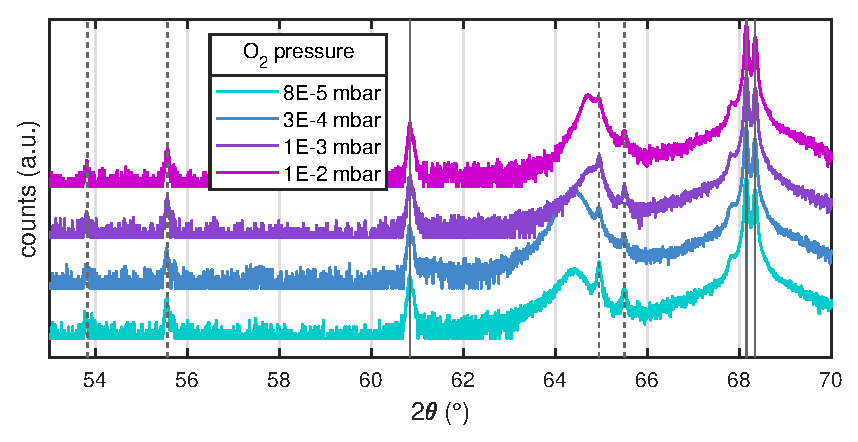
\includegraphics{1_pressure_2theta.eps}
    \caption{\thetaomega-patterns of \cro\ thin films deposited on \textit{m}-plane sapphire for various oxygen partial pressures.
    The solid lines indicate (30.0) substrate reflections corresponding to copper radiation, whereas the dashed lines indicate (30.0) substrate reflections corresponding to tungsten radiation.}
    \label{Fig:Results_1_pressure_2theta}
\end{figure}
In the following, the results for the samples produced at four different oxygen partial pressures are analyzed.
In Fig.\,\ref{Fig:Results_1_pressure_2theta}, the \thetaomega-patterns are depicted.
For each pattern, the two peaks (solid line) at around \qty{68}{\degree} correspond to the (30.0) reflection of the \textit{m}-plane oriented sapphire substrate.
The splitting occurs due to the similar wavelength of \ce{Cu}-K\textalpha\textsubscript{1} and \ce{Cu}-K\textalpha\textsubscript{2} radiation.
The additional peaks also stem mainly from the (30.0) reflection of \ce{Al2O3} and are caused by
\ce{W}-L\textbeta\textsubscript{2}-,
\ce{W}-L\textbeta\textsubscript{1}-,
\ce{Cu}-K\textbeta-,
\ce{W}-L\textalpha\textsubscript{1}- and
\ce{W}-L\textalpha\textsubscript{2}-radiation (increasing angles).\footnote{
    %TODO
    \bfseries\textcolor{red}{Klar wäre das besser das im plot an die linien zu schreiben, aber das war mir irgendwie zu auffändig es schön zu machen. Gehts auch so?}
}
In the vicinity of the calculated peak position for the (30.0) reflection of \cro\ (cf.~\ref{tab:d_strained}), there is a peak observed for each sample, indicating that the \textalpha-phase of \cro\ is present.
Note that the peak position is varying depending on the chosen oxygen partial pressure.
The difference to the expected peak position $2\theta_0$ is expressed as \gls{oop}\ strain $\epsilon_{zz}$ using the Bragg equation Equ.\,\ref{Equ:Theory_BraggCondition} and then
\begin{equation}
    \label{Equ:Results_oop_strain_def}
    \epsilon_{zz}
    =\frac{d-d_0}{d_0}
    =\left(\frac{1}{\sin(2\theta/2)}-\frac{1}{\sin(2\theta_0/2)}\right)
    \cdot\sin(2\theta_0/2)\,.
\end{equation}
In Fig.\,\ref{Fig:Results_1_both_strainFWHM}a, the calculated strain is shown in dependence of the corresponding oxygen partial pressure.
The strain decreases from approx.\ \qty{0.95}{\percent} to \qty{0.45}{\percent} with increasing pressure.
This strain reduction may therefore be the result of increased background gas scattering which results in less kinetic energy of the specimen reaching the heated substrate (cf.~\ref{Sec:Methods_pld}).
\begin{figure}
    \centering
    \begin{tabular}{ll}
        \textbf{(a)}&\textbf{(b)} \figSpace\\
        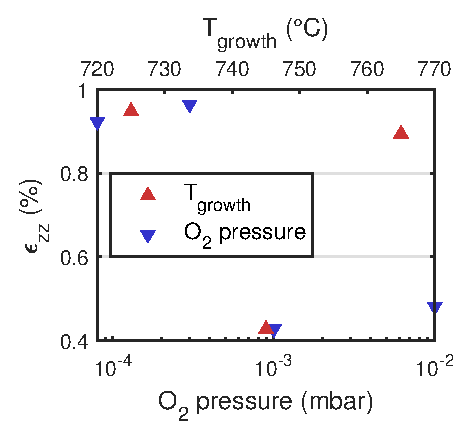
\includegraphics[align=c]{1_both_strain.eps}    
        &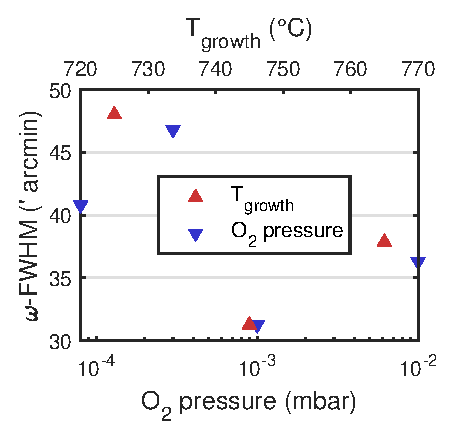
\includegraphics[align=c]{1_both_FWHM.eps}
    \end{tabular}
    \caption{
        \textbf{(a)} \gls{oop}\ strain calculated with Equ.\,\ref{Equ:Results_oop_strain_def} and \textbf{(b)} \textomega-FWHMs for samples from growth temperature series (red triangles, top \textit{x}-axis) and oxygen partial pressure series (blue triangles, bottom \textit{x}-axis).
        }
    \label{Fig:Results_1_both_strainFWHM}
\end{figure}

%! omega-scans
For each sample, the $2\theta$ angle was fixed to the observed (30.0) reflection of \cro\ and an \textomega-scan was performed.
The \glspl{FWHM} of the \textomega-patterns (henceforth \enquote{\textomega-FWHM}) are depicted in
    Fig.\,\ref{Fig:Results_1_both_strainFWHM}b.
The values vary between approx.\ \qtylist{30;50}{\arcminute} and show a dependence on oxygen partial pressure, which is less pronounced compared with \gls{oop}\ strain
    (Fig.\,\ref{Fig:Results_1_both_strainFWHM}a).
Still, since \textomega-FWHM is connected to the mosaicity of the thin film, higher oxygen partial pressures yield slightly better crystal qualities.
Note that due to the fact that an oxygen partial pressure of \qty{1e-3}{\milli\bar} yielded the best crystal quality, this value is used for future deposition processes.

%! phi-scan
To probe for rotational domains of the thin films, \textphi-scans were performed by fixing $2\theta$ and $\omega$ to the corresponding angles of the (30.6) plane of \cro, which has an inclination angle of \qty{32.4}{\degree} with respect to the (30.0) plane.
The diffraction patterns are depicted in Fig.\,\ref{Fig:Results_1_phiScan}.
The observed peaks of the thin film align with the peaks of the single crystal substrate, indicating that the film has no in-plane rotation with respect to the substrate.
Furthermore, the absence of additional peaks indicates that there exists only a single domain of the thin film.
\begin{figure}
    \centering
    \includegraphics{1_both_phi.eps}
    \caption{Diffraction patterns of \textphi-scans performed on the inclined (30.6) reflections for \textit{m}-plane \cro\ (darker color) and \ce{Al2O3} (brighter color).
    The diffraction patterns cover the samples from variation of oxygen partial pressure (teal to blue colored) and variation of growth temperature (red to yellow colored).
    }
    \label{Fig:Results_1_phiScan}
\end{figure}

%! growth rates
The growth rate $g$ varies between \qtylist{3;7}{\pm\per\pulse} and is depicted in Fig.\,\ref{Fig:Results_1_growthRates_photograph}a.
No systematic dependence on the oxygen partial pressure can be observed.
\begin{figure}
    \centering
    \begin{tabular}{ll}
        \textbf{(a)} & \textbf{(b)} \figSpace\\
        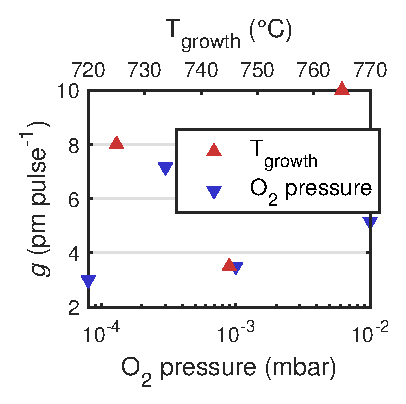
\includegraphics[align=c]{1_both_growthrate.eps}
        &\includegraphics[align=c]{camera_initial.eps}
    \end{tabular}
    \caption{
        \textbf{(a)} Growth rates $g$ for samples from growth temperature series (red triangles, top \textit{x}-axis) and oxygen partial pressure series (blue triangles, bottom \textit{x}-axis).
        \textbf{(b)} Image of the samples produced at different oxygen partial pressures and different growth temperatures.
        }
    \label{Fig:Results_1_growthRates_photograph}
\end{figure}

%! Transmission
The transmission spectra of two selected \cro\ thin films are shown in Fig.\,\ref{Fig:Results_1_transmission}a.
The samples are not fully transparent in the visible spectrum and they exhibit a greenish tint, as can also be seen in Fig.\,\ref{Fig:Results_1_growthRates_photograph}b.
% fitting with indirect gap: cheng 1996, al-kuhaili2007 (^1/2)
% fitting with direct gap: farrell 2015 (^2)
% mi2018 states cr2o3 is a direct bandgap semiconductor
To determine the onset of absorption $E_\tau$, a \textsc{Tauc}-plot (Fig.\,\ref{Fig:Results_1_transmission}b) is utilized (cf.~\ref{Sec:Methods_transmission}).
The exponent is chosen to be $\frac{1}{2}$, resulting in a representation of $(\alpha E)^2$ vs.\ $E$.
Although the publications used for reference in this work support the direct transition nature of \cro\ 
    \cite{farrell2015,mi2018},
it has to be noted that there exist studies determining the optical band gap of \cro\ by applying an exponent of 2, assuming an indirect band gap transition for \cro\ 
    \cite{cheng1996,al-kuhaili2007}.
Fitting the linear regime in the onset of absorption results in $E_\tau\approx\qty{3.7}{\eV}$ for both samples, which differ in strain and \textomega-FWHM by a factor of approx. 2 and 0.3, respectively.
\begin{figure}
    \centering
    \begin{tabular}{c}
        \multicolumn{1}{l}{\textbf{(a)}}\figSpace\\
        \includegraphics[align=t]{1_pressure_transmission.pdf}\figSpace\\
        \multicolumn{1}{l}{\textbf{(b)}}\figSpace\\
        \includegraphics[align=t]{1_pressure_tauc.pdf}
    \end{tabular}
    \caption{\textbf{(a)} Transmission spectra of two selected \cro\ thin films, deposited with different oxygen partial pressures. The spectra are normalized to a corresponding uncoated \textit{m}-plane sapphire substrate.
    \textbf{(b)} \textsc{Tauc}-plot of the above-mentioned samples.
    It is assumed that \cro\ has a direct bandgap
        \cite{farrell2015,mi2018}.
    }
    \label{Fig:Results_1_transmission}
\end{figure}
    \subsubsection{Growth Temperature Variation on \textit{m}-plane Sapphire}
        In the following, the results for the three samples produced at different growth temperatures are presented.
In addition to the oxygen partial pressure, the influence of growth temperature is investigated.  
%! 2theta-omega
Similar to the previous results, the (30.0) reflection of the \textalpha-phase of \cro\ can be observed (Fig.\,\ref{Fig:Results_1_temperature_2theta}).
% Note that the additional peaks are corresponding to the (30.0) reflection of the substrate and stem from various radiation wavelengths.
The calculated \gls{oop}\ strain is shown in Fig.\,\ref{Fig:Results_1_pressureTemperature_yyaxis_strainOmega}b and a large spread of strain can be observed, varying between \qtylist{0.4;1}{\percent}.
Note that there is no systematic dependence on growth temperature.
\begin{figure}
    \centering
    \includegraphics{1_temperature_2theta_labelled.pdf}
    \caption{
        \thetaomega-pattern of \cro\ thin films deposited on \textit{m}-plane sapphire for three different growth temperatures.
        The gray solid lines indicate (30.0) substrate reflections corresponding to copper radiation, whereas the gray dashed lines indicate (30.0) substrate reflections corresponding to tungsten radiation.
        The red line corresponds to the predicted (30.0) reflection of \cro.
    }
    \label{Fig:Results_1_temperature_2theta}
\end{figure}
%! omega
The \textomega-FWHMs of the \cro\ (30.0) reflection are shown in Fig.\,\ref{Fig:Results_1_pressureTemperature_yyaxis_strainOmega}b and exhibit a similar spread as the samples with varying oxygen partial pressure, but similar to the \gls{oop}\ strain, no dependence on growth temperature is observed.
%! phi-scan
The \textphi-scans (Fig.\,\ref{Fig:Results_1_phiScan}) show that the thin films are in-plane aligned with the respective substrate and that no rotational domains are present.
%! growth rate
Finally, the growth rate varies between \qtylist{3.5;10}{\pm\per\pulse} with no observable dependence on growth temperature.
    \subsubsection{Influence of Growth Rate on Crystal Structure}
        %! Why is there another explanation needed?
It has to be noted that there is a large spread in strain, \textomega-FWHM and growth rate for the samples that were deposited at different growth temperatures.
The range of temperature variation was only \qty{40}{\degreeCelsius} and has no significant influence on the distribution of strain and \textomega-FWHM (Fig.\,\ref{Fig:Results_1_pressureTemperature_yyaxis_strainOmega}b).
Note that for the last two samples produced with heater temperatures of $T=\qty{725}{\degreeCelsius}$ and $T=\qty{765}{\degreeCelsius}$, respectively, the pulse number was increased to \qty{40000}{pulses}, leading to thicker samples.
But the crystal structure does not depend on thickness either (not shown).
Because all the other process parameters were kept the same, this indicates that another parameter influences the crystal quality.
This is supported by the fact that the growth rate correlates with the magnitude of strain and \textomega-FWHM, as can be seen in Fig.\,\ref{Fig:Results_1_growthRate_process}a (the outlier with low growth rate but high strain will be explained below).
Note that at this point, the growth rate cannot be deconvoluted from the thin film thickness.
Therefore, it is not clear whether the thickness or the reduced growth rate influences the crystal quality.
% Although strain is related to \textomega-FWHM, it has to be noted that for a small regime of \gls{oop}\ strain around approx.\ \qty{0.9}{\percent}, the \textomega-FWHM scatters between approx.\ \qty{37}{\arcminute} and \qty{47}{\arcminute}.

%! importance of process order
The origin of the varying growth rate -- and therefore varying crystal quality -- can be found when taking the number of processes into account that were performed before a specific process.
In Fig.\,\ref{Fig:Results_1_growthRate_process}b, the growth rate is visualized depending on the order of sample fabrication.
It is also indicated when, the laser entrance window has been cleaned.
It is common practice to clean the latter every couple of processes due to coating with target material which absorbs laser energy.
E.g., in the case of \ce{ZnO}, even after \qty{100000}{pulses}, no significant influence can be observed on the transmission of laser energy.
But from Fig.\,\ref{Fig:Results_1_growthRate_process}b it becomes clear that this should be done much more frequently when working with \cro.
Note that the laser has a wavelength of \qty{248}{\nm}, corresponding to \qty{5.0}{\eV}, which is not transmitted by \cro\ thin films\footnote{
    To be precise, the transmission spectrum in Fig.\,\ref{Fig:Results_1_transmission}a is recorded for \textit{m}-plane oriented \textit{crystalline} \cro\ thin films. This may not be the present phase when \cro\ deposits on the (colder) window made out of glass, where it may form an amorphous phase.
},
as can be seen in Fig.\,\ref{Fig:Results_1_transmission}a.
Therefore, the increasing coating of the laser entrance window with each new process absorbs a large amount of laser pulse energy, resulting in less fluence on the PLD target.
This results in less ablated target material and less kinetic energy of the ablated species, which leads to a reduced growth rate and different crystal growth conditions that have less strain and \textomega-FWHM as a result.
\begin{figure}
    \centering
    \begin{tabular}{ll}
        \textbf{(a)} & \textbf{(b)} \figSpace\\
        \includegraphics[align=c]{1_initial_strainOmegaCorrelation.eps}
        &\includegraphics[align=c]{1_initial_window.eps}
    \end{tabular}
    \caption{
        \textbf{(a)} Correlation of \textomega-FWHM with \gls{oop}\ strain, as well as correlation of both with growth rate $g$ (false color).
        The dashed line is a linear fit serving as guide to the eye.
        The outlier with low growth rate but large strain can be explained by accounting for the low oxygen partial pressure of \qty{8e-5}{\milli\bar} for this sample.
        This results in larger kinetic energy of the plasma species.
        \textbf{(b)}~ Growth rate depending on order of sample fabrication.
    }
    \label{Fig:Results_1_growthRate_process}
\end{figure}

%! compatable with oxygen explanation
This explanation is supported by the dependence of crystal quality on oxygen partial pressure (cf.\ Fig.\,\ref{Fig:Results_1_pressureTemperature_yyaxis_strainOmega}a).
There, the increasing crystal quality with higher oxygen pressures is attributed to the increased background gas scattering resulting in less kinetic energy of the plasma material.
This also explains the outlier in Fig.\,\ref{Fig:Results_1_growthRate_process}a, where one sample corresponds to a higher strain and \textomega-FWHM of approx.\ \qty{0.9}{\percent} and \qty{41}{\arcminute}, respectively (black square).
This is not expected when considering the rather small growth rate of \qty{3}{\pm\per\pulse} (\texttt{W6724} in Fig.\,\ref{Fig:Results_1_growthRate_process}b).
But when taking into account that this sample is fabricated at a very low oxygen partial pressure of \qty{8e-5}{\milli\bar}, it becomes clear that although the reduced fluence on the target would generally lower the kinetic energy of the plasma material, the limited scattering with the background gas counteracts this effect, resulting in the observed crystal quality.

%! phi-dependence of strain
It is noteworthy that the observed strain (cf.\ Fig.\,\ref{Fig:Results_1_pressureTemperature_yyaxis_strainOmega}a,b) is distributed around two distinct values of approx.\ \qty{0.4}{\percent} and \qty{0.9}{\percent}.
A prior reported thin film tilt for \textit{m}-plane oriented rhombohedral heterostructures
    \cite{kneiss2021}
may be the reason for this observation:
the samples are installed in the XRD device in such a way that the \textit{c}-axis is either parallel or orthogonal to the scattering plane.
This orientation is arbitrary, and thus the (expected) thin film tilt is either along the X-ray beam or perpendicular to it, which could result in unexpected results when calculating the \gls{oop}\ lattice plane distance from the observed peak position.
To check if this is the origin of the observed strain, for two samples of different strain according to Fig.\,\ref{Fig:Results_1_pressureTemperature_yyaxis_strainOmega}, four \thetaomega-scans were performed with incrementing the azimuth by \qty{90}{\degree} after each measurement.
The resulting diffraction patterns are depicited in Fig.\,\ref{Fig:Results_1_checkPhi}.
The strain is independent of azimuth, only the peak intensity is altered by the in-plane rotation of the sample as expected.
For both samples, an azimuth of \qtylist{0;180}{\degree} results in a lower intensity, supporting the hypothesis that the (expected) thin film tilt is perpendicular to scattering plane which results in a deviation from the \gls{bc}.
Therefore, the distribution of observed strain is not a measurement artifact.
\begin{figure}
    \centering
    \includegraphics{1_initial_checkPhiDependence.eps}
    \caption{
        \thetaomega-patterns for two samples in four different azimuths each.
        The black dashed line indicates the expected (30.0) reflection of \cro.
        }
    \label{Fig:Results_1_checkPhi}
\end{figure}

    \subsubsection{Deposition on \textit{c}-, \textit{r}-, \textit{m}- and \textit{a}-plane Sapphire}
        %! theta-omega
For the samples deposited on substrates with different orientation, \thetaomega-patterns were recorded (Fig.\,\ref{Fig:Results_1_w6788_2theta}).
For each sample, the expected substrate peaks are observed:
(00.6) and (00.12) for \textit{c}-plane;
(01.2), (02.4), (03.6) and (04.8) for \textit{r}-plane;
(30.0) for \textit{m}-plane;
(11.0) and (22.0) for \textit{a}-plane.
Several smaller peaks also correspond to those reflections but stem from other X-rays than \ce{Cu}-K\textalpha\ (cf.\ Fig.\,\ref{Fig:Results_1_pressure_2theta}).
The mentioned reflections are also observed for the \cro\ thin film, but with a shift in $2\theta$ position similar to the previously investigated \textit{m}-plane samples (Tab.\,\ref{Tab:Results_1_w6788}).
Note that for \textit{r}-plane, the higher order reflections of \cro\ cannot be observed.
It can be concluded that \cro\ grows in the \textalpha-phase on sapphire substrates of different orientation, where the thin film orientation matches the corresponding substrate.
Henceforth, \enquote{\textit{c}-plane \cro} will refer to a \cro\ thin film deposited on \textit{c}-plane oriented $5\times\qty{5}{\mm\squared}$ sapphire substrates, and so on.
\begin{figure}
    \centering
    \includegraphics{1_W6788_2theta_labeled.eps}
    \caption{\thetaomega-patterns of \cro\ thin films deposited on \textit{c}-, \textit{r}-, \textit{m}- and \textit{a}-plane sapphire.}
    \label{Fig:Results_1_w6788_2theta}
\end{figure}
% consider putting [h] to avoid crashing of table with figure
\begin{table}
    \centering
    \caption{Structural parameters, approximate resistivity at room temperature and activation energy for \cro\ thin films of different orientation.}
    \begin{tabular}{ccccc}
        \toprule
        Plane
            & $\epsilon_{zz}$ (\unit{\percent})
            & \textomega-FWHM (\unit{\arcminute}) 
            & $\rho$ (\unit{\ohm\cm})
            & $E_A$ (\unit{\milli\eV})\\
        \midrule
        \textit{c}  &   1.71    &   42.6    &   3       &   57, 34  \\
        \textit{r}  &   0.72    &   38.4    &   120     &   117     \\
        \textit{m}  &   0.55    &   42.6    &   3600    &   240     \\
        \textit{a}  &   1.41    &   32.4    &   4900    &   259     \\
        \bottomrule
    \end{tabular}
    \label{Tab:Results_1_w6788}
\end{table}
%! Omega-scans
For each sample, \textomega-scans were performed on the (00.6), (02.4), (30.0) and (11.0) reflections for \textit{c}-, \textit{r}-, \textit{m}- and \textit{a}-plane, respectively.
The resulting \textomega-FWHMs are in the range of approx.\ \qty{30}{\arcminute} to \qty{40}{\arcminute} (Tab.\,\ref{Tab:Results_1_w6788}).

%! Resistivity
Because the resistivity of all samples was too high to measure Hall effect, only resistivity measurements (cf.~\ref{Sec:Methods_vanDerPauw}) were performed for several temperatures (Fig.\,\ref{Fig:Results_1_w6788_TdH}).
The resistivity depends strongly on the orientation of the thin film, the resistivities at room temperature are listed in Tab.\,\ref{Tab:Results_1_w6788}.
A difference of more than three orders of magnitude between \textit{c}-plane and \textit{a}-plane samples is observed.
The linear behavior of the \textsc{Arrhenius}-plot\footnote{
    Visualization of $f(T)$ as $f'(\tau)$ with $f'=\log f$ and $\tau=1/T$.
}
indicates a thermally activated mechanism for conductivity, and thus semiconductive behavior.
Note that no further conclusions can be drawn on the conduction mechanisms due to the missing carrier concentration and mobility data.
By assuming a behavior of the form
\begin{equation}
    \label{Equ:Results_1_Arrhenius}
    \rho\propto\exp\left(\frac{E_A}{k_BT}\right)\,,
\end{equation}
with \textsc{Boltzmann} constant $k_B$, an activation energy $E_A$ can be estimated.
Those energies are also listed in Tab.\,\ref{Tab:Results_1_w6788}.
For \textit{c}-plane \cro, two linear regimes can be distinguished, favoring a dependence of the form
\begin{equation}
    \label{Equ:Results_1_Arrhenius2}
    \rho\propto a\exp\left(\frac{E_{A,1}}{k_BT}\right)
    +b\exp\left(\frac{E_{A,2}}{k_BT}\right)\,,
\end{equation}
thus two activation energies are determined.
\begin{figure}
    \centering
    \includegraphics{1_W6788_resistivityTempDep.eps}
    \caption{
        Temperature dependent resistivity measurements for samples with different orientations.
    }
    \label{Fig:Results_1_w6788_TdH}
\end{figure}

\subsection{Conclusion}
    \textit{m}-plane \cro\ thin films can be deposited over a wide range of oxygen partial pressure of more than 2 orders of magnitude.
It turned out that the main influence on the crystal quality correlates with the growth rate and is due to a variation of the laser pulse fluence on the target.
Nevertheless, an oxygen partial pressure of \qty{1e-3}{\milli\bar} and a growth temperature of \qty{750}{\degreeCelsius} are chosen for deposition of subsequent thin films.
\textalpha-\cro\ could also deposited on \textit{c}-, \textit{r}- and \textit{a}-plane sapphire, with the thin films crystallizing in the respective orientation.
Note that all deposited thin films showed a discrepancy between observed \gls{oop}\ lattice plane distance and values predicted from Tab.\,\ref{Tab:sesquiLatticeConstants}.
The conductivity is strongly dependent on the crystal orientation and was very low for the prismatic orientations, but with \qty{0.3}{\siemens\per\cm} three orders of magnitude higher for the basal orientation.
    % \clearpage

%! (2)
    The resistivity of the \cro\ thin films showed strong dependence on thin film orientation.
To improve and taylor the conductivity, it is tried to incorporate acceptors into the \textit{p}-type material.
The elements chosen for this are \ce{Cu} and \ce{Zn}, because doping has already been accomplished on \textit{c}-plane sapphire with magnesium via \ce{MgO}
    \cite{farrell2015}.
Furthermore, it is tried to improve the ohmic behavior of the contacts of the thin films.

\subsection{Experiment}
    %! measurements
\comment{\thetaomega-scans were performed for every sample, but \textomega-scans for \textit{c}- and \textit{r}-plane samples only.
The thickness was determined using spectroscopic ellipsometry.
Resistivity measurements at room temperature were done using the \textsc{Pauw} method, which was also applied when conducting temperature dependent resistivity measurements on one \textit{c}-plane sample of each target.
Note that the effect of infrequent cleaning of the laser entrance window that was described in \ref{Sec:Results_Preliminary} was discovered during the execution of those experiments, which is why the samples produced from the ZnO-doped (high) target were the only ones for which this effect could be prevented.
Furthermore, \qty{40000}{pulses} were applied for the samples fabricated from the CuO-doped and ZnO-doped (low) target, as well as one sample from the batch made with the ZnO-doped (high) target.
All other samples from this batch were deposited with \qty{30000}{pulses}.}
\subsection{Results}
    \subsubsection{Laser Position Variation for Different Targets}
        %! Growth rates
To investigate the growth rate, spectroscopic ellipsometry measurements were performed to determine the thickness.
The according growth rates of the samples produced from the \ce{CuO}-doped and \ce{ZnO}-doped (low) target are depicted in Fig.\,\ref{Fig:Results_2_windowCleaning}.
The growth rates vary between 3 and \qty{6}{\pm\per\pulse} and depend strongly on the number of deposition processes that were conducted before.
By cleaning the laser entrance window after three processes, and thus reducing laser energy absorption, the growth rate is doubled, which is non-negligible.
This is similar to the results obtained in chapter \ref{Sec:Results_Preliminary}.
\begin{figure}
    \centering
    \includegraphics{2_doped0.01_window.eps}
    \caption{
        Growth rate depending on the process order for the samples fabricated from the CuO-doped and ZnO-doped (low) target.
        It is indicated when the laser entrance windows was cleaned.
    }
    \label{Fig:Results_2_windowCleaning}
\end{figure}

To circumvent the effect of the window blinding with each process, the window was cleaned after each process for the samples produced from the ZnO-doped (high) target.
The growth rates depending on the fabrication order for the those samples are depicted in Fig.\,\ref{Fig:Results_2_yToComposition}b.
However, note that the growth rate still varies from approx.\ \qtyrange{2.5}{6.5}{\pm\per\pulse}, even though the laser entrance window was cleaned after each process.
So this variation in growth rate must be traced back to another effect.
Only the first sample was fabricated with \qty{40000}{pulses}, which explains the increment of growth rate between the first and second process:
% Due to the higher number of pulses, the laser entrance window gets more coated and thus the last \qty{10000}{pulses} reduce the average growth rate.
The condensation of material on the laser entrance window yields a decreasing growth rate over time. This has a strong effect on the overall growth rate calculated for the complete process.
Furthermore, the second process was done with $r_\mathrm{PLD}=\qty{6}{\mm}$, which is rather outside compared to the 1st, 3rd and 4th process with \qtylist{3;4;2}{\mm}, respectively.
This results in a larger total ablated area and in less target degradation.
Therefore, the hypothesis is that target degradation during deposition has an influence on the growth rate.
% This is supported by the observation of incremental reduction of growth rate for processes 1, 5 and 6.
To systematically investigate this, three processes were conducted at the same radius, namely process 1, 5 and 6.
Note that all these samples were fabricated with $r_\mathrm{PLD}=\qty{3}{\mm}$ and otherwise the same deposition parameters.
The only variation is that tracks are carved into the target by the laser (Fig.\,\ref{Fig:Results_2_photoTarget}c).
This is probably the reason for a crucial change in plasma dynamics and therefore a reduction of the growth rate from approx.\ \qtyrange{5}{2.5}{\pm\per\pulse}.
\begin{figure}
    \centering
    \begin{tabular}{lll}
        \textbf{(a)} & \textbf{(b)} & \textbf{(c)} \figSpace \\
        \includegraphics[width=.3\linewidth]{photo_CuO.eps}
        & \includegraphics[width=.3\linewidth]{photo_ZnO(L).eps}
        & \includegraphics[width=.3\linewidth]{photo_ZnO(H).eps}
    \end{tabular}
    \caption{Photograph of the \textbf{(a)} CuO-doped, \textbf{(b)} ZnO-doped (low) and \textbf{(c)} ZnO-doped (high) target.
    The CuO-doped target broke during the last process it was used in.
    The silverish tint is presuambly due to the formation of metallic chromium oxide \ce{CrO2} on the target surface.}
    % The tracks carved into target at the frequently applied radial laser positions are visible.}
    \label{Fig:Results_2_photoTarget}
\end{figure}

%! resistivity
\newpage
To probe the conductivity of the fabricated samples, resistivity measurements were performed using the \textsc{Pauw} methods.
Only \textit{r}- and \textit{c}-plane samples were investigated, because the prismatic planes exhibited resistances of several \unit{\giga\ohm} or higher, when measured with a multimeter, as the \textsc{Hall}-effect measurement setup at the semiconductors group is not designed to measure such high resistivities.
In Fig.\,\ref{Fig:Results_2_rho}a, the measured resistivity $\rho$ at room temperature depending on the predicted dopant concentration $x_D$ is depicted. 
From the unsystematic variation in resistivity (\qtyrange{2}{500}{\ohm\cm}), it can be concluded that the attempt of doping the \cro\ thin films resulted in no improvement of conductivity.
Using the two targets with different concentration of \ce{ZnO} in the inner ellipse, no change was observed when adjusting $x_D$ between \qty{0.001}{\percent} and \qty{1}{\percent}.
In particular, note the aforementioned samples (1, 5 and 6 in Fig.\,\ref{Fig:Results_2_yToComposition}b) that were fabricated with the same growth condition $r_\mathrm{PLD}=\qty{3}{\mm}$, corresponding to the triangles in Fig.\,\ref{Fig:Results_2_rho}a at approx.\ $x_D=\qty{1}{\percent}$:
% Note the aforementioned samples that were all fabricated with $r_\mathrm{PLD}=\qty{3}{\mm}$ on the ZnO-doped (high) target, corresponding to the triangles in Fig.\,\ref{Fig:Results_2_rho}a at approx.\ $x_D=\qty{1}{\percent}$:
here, the same process parameters yield samples differing in resistivity by 2 orders of magnitude.
Because those samples showed different growth rates due to target degradation, it is plausible that these altered growth dynamics also influence the conductivity.
\begin{figure}
    \centering
    \begin{tabular}{c}
        \multicolumn{1}{l}{\textbf{(a)}} \figSpace \\
        \includegraphics{2_doped_rhoVScomp.eps} \figSpace \\        
        \multicolumn{1}{l}{\textbf{(b)}} \figSpace \\
        \includegraphics{2_doped_rhoVSomega.eps}
    \end{tabular}
    \caption{
        \textbf{(a)} Resistivity vs.\ predicted dopant concentration for \textit{c}- and \textit{r}-plane samples fabricated from all three radially segmented targets.
        \textbf{(b)} Resistivity vs.\ \textomega-FWHM of the aforementioned samples.
        Note that the \textit{r}-plane samples fabricated from the ZnO-doped (high) target did not exhibit sufficient peak intensity to determine the \textomega-FWHM.
    }
    \label{Fig:Results_2_rho}
\end{figure}

%! Omega scans
Because in the previous chapter \ref{Sec:Results_Preliminary} it was shown that the growth rate is correlating to the \textomega-FWHM, Rocking scans were performed on the (00.6) and (02.4) reflection for \textit{c}-plane and \textit{r}-plane samples, respectively.
The extracted \textomega-FWHMs are depicted in Fig.\,\ref{Fig:Results_2_omega} depending on the growth rate for the respective process.
A general trend is that the crystallinty increases for lower growth rates, namely for a growth rate of \qty{3.4}{\pm\per\pulse}, a \textomega-FWHM of \qty{4}{\arcminute} (\qty{240}{\arcsecond}) can be achieved.
It is irrelevent, whether this reduction in growth rate is due to lower fluence on the laser target due to infrequent window cleaning (CuO-doped and ZnO-doped (low) target) or due to target degradation (ZnO-doped (high) target).
The better FWHM is achieved for \textit{c}-plane samples.
Note that for the deposition of \cro\ on \textit{r}-plane sapphire from the ZnO-doped (high) target, no thin film peaks in \thetaomega-scans were observed (Fig.\,\ref{Fig:App_2_ZnO_H_rAmorphous}).
Those X-ray-amorphous films are presumably a result of the drastically altered plasma dynamics due to target degradation.
\begin{figure}
    \centering
    \includegraphics{2_doped_omega.eps}
    \caption{\textomega-FWHM for \textit{c}- and \textit{r}-plane samples that were fabricated from the three radially segmented targets.}
    \label{Fig:Results_2_omega}
\end{figure}

{% fix non-breaking of Fig reference
\sloppy
To investigate the influence of crystal quality on the electrical properties, in Fig.\,\ref{Fig:Results_2_rho}b, the resistivity depending on the \textomega-FWHM is depicted. % overfull hbox fix: \, --> 
It becomes clear that a higher mosaicity results in higher conductivity.
Since more dislocations correspond to more crystal defects (cf.\ section \ref{Sec:Theory_Relaxed}), this result is in accordance to the predicted influence of crystal defects on the electrical properties of \cro\ thin films (cf.\ section \ref{Sec:Cr2O3}).
It has to be noted that this effect is less pronounced for \textit{r}-plane samples compared to \textit{c}-plane samples, where resistivies as low as \qty{1.9}{\ohm\cm} can be achieved for an \textomega-FWHM of \qty{40}{\arcminute}.
Furthermore, this does not explain why \textit{m}- and \textit{a}-plane \cro\ exhibit such high resistivity, because their \textomega-FWHM is comparable to the basal and pyramidal orientations (cf.\ Tab.\,\ref{Tab:Results_1_w6788}).
\par}

%! temperature-dependent Hall
For each target, one \textit{c}-plane sample with presumably highest doping concentration (smallest $r_\mathrm{PLD}$) was chosen to perform temperature dependent resistivity measurements in the range of \qtyrange{40}{390}{\kelvin} (Fig.\,\ref{Fig:Results_2_TdH}).
For all samples, an \textsc{Arrhenius}-like behavior is observed with two linear regimes above and below \qty{100}{\kelvin}, respectively.
By applying \eqref{Equ:Results_1_Arrhenius2}, two activation energies can be extracted that are listed in Tab.\,\ref{Tab:Results_2_activationEnergy}.
Note that there is no significant difference between the undoped and doped samples.
Furthermore, the samples with the smallest ablation radius for each target were chosen, and not the samples with the highest conductivity for each batch.
Therefore, the data in Fig.\,\ref{Fig:Results_2_TdH} does not indicate that samples from the Cu-doped target have lower conductivity per se.
\begin{figure}
    \centering
    \includegraphics{2_doped_TdH.eps}
    \caption{
        Temperature dependent resistivity measurements for \textit{c}-plane samples fabricated from the different radially segmented targets, as well as a pure \cro\ target.
        The clipping of the sample from the CuO-doped target (green squares) is due to the limited resolution of the measurement device and the artifact nature of this saturation is confirmed by repeated measurements with different current applied during measurement (not shown).
    }
    \label{Fig:Results_2_TdH}
\end{figure}
\begin{table}
    \centering
    \caption{Activation energies $E_A$ extracted from the linear regimes in the temperature dependent resistivity measurements (Fig.\,\ref{Fig:Results_2_TdH}).
    }
    \begin{tabular}{ccc}
        \toprule
        target & \multicolumn{2}{c}{$E_A$ (\unit{\milli\eV})} \\
        & $<\qty{100}{\kelvin}$ & $>\qty{100}{\kelvin}$ \\
        \midrule
        CuO-doped           &   53   &   83  \\
        ZnO-doped (low)     &   35    &   61  \\
        ZnO-doped (high)    &   31    &   50  \\
        pure \cro           &   35    &   54  \\
        \bottomrule
    \end{tabular}
    \label{Tab:Results_2_activationEnergy}
\end{table}

%! Theta-omega
\newpage
Even though the doping resulted in no improvement of the electrical properties of the thin films, the several samples fabricated at different growth conditions -- due to infrequent laser window cleaning and target degradation -- may serve as an insight into the \gls{oop}\ strain that was already observed in chapter \ref{Sec:Results_Preliminary}.
The \gls{oop}\ strain dependent on the growth rate is depicted in Fig.\,\ref{Fig:Results_2_strain}a and was determined from \cro\ peak positions in \thetaomega\ patterns.
For \textit{m}- and \textit{a}-plane, the hypothesis of increasing strain with increasing growth rate can be confirmed.
However, the slope of this relation differs depending on the target:
the samples fabricated from the CuO-doped target showed less strain depending on growth rate than the samples fabricated from the ZnO-doped (high) target.
This may be explained by the fact that the target degradation for the former (cf.\ Fig.\,\ref{Fig:Results_2_photoTarget}a) was not so pronounced when compared to the latter (cf.\ Fig.\,\ref{Fig:Results_2_photoTarget}c).
\begin{figure}
    \centering
    \begin{tabular}{cc}
        \multicolumn{1}{l}{\textbf{(a)}} \figSpace \\
        \includegraphics{2_doped_strain.eps} \figSpace \\
        \multicolumn{1}{l}{\textbf{(b)}} \figSpace \\
        \includegraphics{2_doped_strainOmegaCorrelation.eps} \\        
    \end{tabular}
    
    \caption{
        \textbf{(a)} Strain extracted from the peak positions in \thetaomega-scans for samples fabricated from the three radially segmented targets.
        \textbf{(b)} Correlation between strain and \textomega-FWHM for \textit{c}- and \textit{r}-plane samples.
        The samples fabricated at different growth temperatures are also included.}

    \label{Fig:Results_2_strain}
\end{figure}

A reverse behavior is observed for \textit{c}-plane samples: the strain is increasing with higher growth rates.
But compared to \textit{m}- and \textit{a}-plane, there is no significant difference between the samples fabricated from different targets.
This leads to the assumption that the plasma dynamics do not determine the \gls{oop}\ strain for this orientation.
It has to be noted that due to the constant pulse number, a change in growth rate corresponds to a change in thickness of the thin films.
Therefore, it may be possible that the strain of the thin samples (low growth rate) is due to pseudomorphic growth on the corresponding \ce{Al2O3} substrate.
Note that this leads not to the conclusion that the origin of the strain in \textit{m}- and \textit{a}-plane samples is also pseudomorphic growth:
There, the thicker samples show more strain which is not expected because far away from the interface, dislocations should form to propagate relaxed growth.
For \textit{r}-plane samples, the overall strain is smaller and shows a less pronounced trend similar to \textit{m}- and \textit{a}-orientation.
Because \textit{r}-plane has both basal and prismatic character, both thickness and plasma dynamics effects may contribute to the observed strain.

%! Correlation
The qualitative difference between \textit{c}-plane and the other orientations can also be observed in Fig.\,\ref{Fig:Results_2_strain}b, where the \textomega-FWHM is shown depending on the \gls{oop}\ strain.
Compared to the previous results (cf. Fig.\,\ref{Fig:Results_1_growthRate_process}a), both factors characterizing crystal quality (strain and \textomega-FWHM) are not minimized simultaneously.
    % For final document:
    % The resistivity of the \cro\ thin films showed strong dependence on thin film orientation.
To improve and taylor the conductivity, it is tried to incorporate acceptors into the \textit{p}-type material.
The elements chosen for this are \ce{Cu} and \ce{Zn}, because doping has already been accomplished on \textit{c}-plane sapphire with magnesium via \ce{MgO}
    \cite{farrell2015}.
Furthermore, it is tried to improve the ohmic behavior of the contacts of the thin films.

\subsection{Experiment}
    %! measurements
\comment{\thetaomega-scans were performed for every sample, but \textomega-scans for \textit{c}- and \textit{r}-plane samples only.
The thickness was determined using spectroscopic ellipsometry.
Resistivity measurements at room temperature were done using the \textsc{Pauw} method, which was also applied when conducting temperature dependent resistivity measurements on one \textit{c}-plane sample of each target.
Note that the effect of infrequent cleaning of the laser entrance window that was described in \ref{Sec:Results_Preliminary} was discovered during the execution of those experiments, which is why the samples produced from the ZnO-doped (high) target were the only ones for which this effect could be prevented.
Furthermore, \qty{40000}{pulses} were applied for the samples fabricated from the CuO-doped and ZnO-doped (low) target, as well as one sample from the batch made with the ZnO-doped (high) target.
All other samples from this batch were deposited with \qty{30000}{pulses}.}
\subsection{Results}
    \subsubsection{Laser Position Variation for Different Targets}
        %! Growth rates
To investigate the growth rate, spectroscopic ellipsometry measurements were performed to determine the thickness.
The according growth rates of the samples produced from the \ce{CuO}-doped and \ce{ZnO}-doped (low) target are depicted in Fig.\,\ref{Fig:Results_2_windowCleaning}.
The growth rates vary between 3 and \qty{6}{\pm\per\pulse} and depend strongly on the number of deposition processes that were conducted before.
By cleaning the laser entrance window after three processes, and thus reducing laser energy absorption, the growth rate is doubled, which is non-negligible.
This is similar to the results obtained in chapter \ref{Sec:Results_Preliminary}.
\begin{figure}
    \centering
    \includegraphics{2_doped0.01_window.eps}
    \caption{
        Growth rate depending on the process order for the samples fabricated from the CuO-doped and ZnO-doped (low) target.
        It is indicated when the laser entrance windows was cleaned.
    }
    \label{Fig:Results_2_windowCleaning}
\end{figure}

To circumvent the effect of the window blinding with each process, the window was cleaned after each process for the samples produced from the ZnO-doped (high) target.
The growth rates depending on the fabrication order for the those samples are depicted in Fig.\,\ref{Fig:Results_2_yToComposition}b.
However, note that the growth rate still varies from approx.\ \qtyrange{2.5}{6.5}{\pm\per\pulse}, even though the laser entrance window was cleaned after each process.
So this variation in growth rate must be traced back to another effect.
Only the first sample was fabricated with \qty{40000}{pulses}, which explains the increment of growth rate between the first and second process:
% Due to the higher number of pulses, the laser entrance window gets more coated and thus the last \qty{10000}{pulses} reduce the average growth rate.
The condensation of material on the laser entrance window yields a decreasing growth rate over time. This has a strong effect on the overall growth rate calculated for the complete process.
Furthermore, the second process was done with $r_\mathrm{PLD}=\qty{6}{\mm}$, which is rather outside compared to the 1st, 3rd and 4th process with \qtylist{3;4;2}{\mm}, respectively.
This results in a larger total ablated area and in less target degradation.
Therefore, the hypothesis is that target degradation during deposition has an influence on the growth rate.
% This is supported by the observation of incremental reduction of growth rate for processes 1, 5 and 6.
To systematically investigate this, three processes were conducted at the same radius, namely process 1, 5 and 6.
Note that all these samples were fabricated with $r_\mathrm{PLD}=\qty{3}{\mm}$ and otherwise the same deposition parameters.
The only variation is that tracks are carved into the target by the laser (Fig.\,\ref{Fig:Results_2_photoTarget}c).
This is probably the reason for a crucial change in plasma dynamics and therefore a reduction of the growth rate from approx.\ \qtyrange{5}{2.5}{\pm\per\pulse}.
\begin{figure}
    \centering
    \begin{tabular}{lll}
        \textbf{(a)} & \textbf{(b)} & \textbf{(c)} \figSpace \\
        \includegraphics[width=.3\linewidth]{photo_CuO.eps}
        & \includegraphics[width=.3\linewidth]{photo_ZnO(L).eps}
        & \includegraphics[width=.3\linewidth]{photo_ZnO(H).eps}
    \end{tabular}
    \caption{Photograph of the \textbf{(a)} CuO-doped, \textbf{(b)} ZnO-doped (low) and \textbf{(c)} ZnO-doped (high) target.
    The CuO-doped target broke during the last process it was used in.
    The silverish tint is presuambly due to the formation of metallic chromium oxide \ce{CrO2} on the target surface.}
    % The tracks carved into target at the frequently applied radial laser positions are visible.}
    \label{Fig:Results_2_photoTarget}
\end{figure}

%! resistivity
\newpage
To probe the conductivity of the fabricated samples, resistivity measurements were performed using the \textsc{Pauw} methods.
Only \textit{r}- and \textit{c}-plane samples were investigated, because the prismatic planes exhibited resistances of several \unit{\giga\ohm} or higher, when measured with a multimeter, as the \textsc{Hall}-effect measurement setup at the semiconductors group is not designed to measure such high resistivities.
In Fig.\,\ref{Fig:Results_2_rho}a, the measured resistivity $\rho$ at room temperature depending on the predicted dopant concentration $x_D$ is depicted. 
From the unsystematic variation in resistivity (\qtyrange{2}{500}{\ohm\cm}), it can be concluded that the attempt of doping the \cro\ thin films resulted in no improvement of conductivity.
Using the two targets with different concentration of \ce{ZnO} in the inner ellipse, no change was observed when adjusting $x_D$ between \qty{0.001}{\percent} and \qty{1}{\percent}.
In particular, note the aforementioned samples (1, 5 and 6 in Fig.\,\ref{Fig:Results_2_yToComposition}b) that were fabricated with the same growth condition $r_\mathrm{PLD}=\qty{3}{\mm}$, corresponding to the triangles in Fig.\,\ref{Fig:Results_2_rho}a at approx.\ $x_D=\qty{1}{\percent}$:
% Note the aforementioned samples that were all fabricated with $r_\mathrm{PLD}=\qty{3}{\mm}$ on the ZnO-doped (high) target, corresponding to the triangles in Fig.\,\ref{Fig:Results_2_rho}a at approx.\ $x_D=\qty{1}{\percent}$:
here, the same process parameters yield samples differing in resistivity by 2 orders of magnitude.
Because those samples showed different growth rates due to target degradation, it is plausible that these altered growth dynamics also influence the conductivity.
\begin{figure}
    \centering
    \begin{tabular}{c}
        \multicolumn{1}{l}{\textbf{(a)}} \figSpace \\
        \includegraphics{2_doped_rhoVScomp.eps} \figSpace \\        
        \multicolumn{1}{l}{\textbf{(b)}} \figSpace \\
        \includegraphics{2_doped_rhoVSomega.eps}
    \end{tabular}
    \caption{
        \textbf{(a)} Resistivity vs.\ predicted dopant concentration for \textit{c}- and \textit{r}-plane samples fabricated from all three radially segmented targets.
        \textbf{(b)} Resistivity vs.\ \textomega-FWHM of the aforementioned samples.
        Note that the \textit{r}-plane samples fabricated from the ZnO-doped (high) target did not exhibit sufficient peak intensity to determine the \textomega-FWHM.
    }
    \label{Fig:Results_2_rho}
\end{figure}

%! Omega scans
Because in the previous chapter \ref{Sec:Results_Preliminary} it was shown that the growth rate is correlating to the \textomega-FWHM, Rocking scans were performed on the (00.6) and (02.4) reflection for \textit{c}-plane and \textit{r}-plane samples, respectively.
The extracted \textomega-FWHMs are depicted in Fig.\,\ref{Fig:Results_2_omega} depending on the growth rate for the respective process.
A general trend is that the crystallinty increases for lower growth rates, namely for a growth rate of \qty{3.4}{\pm\per\pulse}, a \textomega-FWHM of \qty{4}{\arcminute} (\qty{240}{\arcsecond}) can be achieved.
It is irrelevent, whether this reduction in growth rate is due to lower fluence on the laser target due to infrequent window cleaning (CuO-doped and ZnO-doped (low) target) or due to target degradation (ZnO-doped (high) target).
The better FWHM is achieved for \textit{c}-plane samples.
Note that for the deposition of \cro\ on \textit{r}-plane sapphire from the ZnO-doped (high) target, no thin film peaks in \thetaomega-scans were observed (Fig.\,\ref{Fig:App_2_ZnO_H_rAmorphous}).
Those X-ray-amorphous films are presumably a result of the drastically altered plasma dynamics due to target degradation.
\begin{figure}
    \centering
    \includegraphics{2_doped_omega.eps}
    \caption{\textomega-FWHM for \textit{c}- and \textit{r}-plane samples that were fabricated from the three radially segmented targets.}
    \label{Fig:Results_2_omega}
\end{figure}

{% fix non-breaking of Fig reference
\sloppy
To investigate the influence of crystal quality on the electrical properties, in Fig.\,\ref{Fig:Results_2_rho}b, the resistivity depending on the \textomega-FWHM is depicted. % overfull hbox fix: \, --> 
It becomes clear that a higher mosaicity results in higher conductivity.
Since more dislocations correspond to more crystal defects (cf.\ section \ref{Sec:Theory_Relaxed}), this result is in accordance to the predicted influence of crystal defects on the electrical properties of \cro\ thin films (cf.\ section \ref{Sec:Cr2O3}).
It has to be noted that this effect is less pronounced for \textit{r}-plane samples compared to \textit{c}-plane samples, where resistivies as low as \qty{1.9}{\ohm\cm} can be achieved for an \textomega-FWHM of \qty{40}{\arcminute}.
Furthermore, this does not explain why \textit{m}- and \textit{a}-plane \cro\ exhibit such high resistivity, because their \textomega-FWHM is comparable to the basal and pyramidal orientations (cf.\ Tab.\,\ref{Tab:Results_1_w6788}).
\par}

%! temperature-dependent Hall
For each target, one \textit{c}-plane sample with presumably highest doping concentration (smallest $r_\mathrm{PLD}$) was chosen to perform temperature dependent resistivity measurements in the range of \qtyrange{40}{390}{\kelvin} (Fig.\,\ref{Fig:Results_2_TdH}).
For all samples, an \textsc{Arrhenius}-like behavior is observed with two linear regimes above and below \qty{100}{\kelvin}, respectively.
By applying \eqref{Equ:Results_1_Arrhenius2}, two activation energies can be extracted that are listed in Tab.\,\ref{Tab:Results_2_activationEnergy}.
Note that there is no significant difference between the undoped and doped samples.
Furthermore, the samples with the smallest ablation radius for each target were chosen, and not the samples with the highest conductivity for each batch.
Therefore, the data in Fig.\,\ref{Fig:Results_2_TdH} does not indicate that samples from the Cu-doped target have lower conductivity per se.
\begin{figure}
    \centering
    \includegraphics{2_doped_TdH.eps}
    \caption{
        Temperature dependent resistivity measurements for \textit{c}-plane samples fabricated from the different radially segmented targets, as well as a pure \cro\ target.
        The clipping of the sample from the CuO-doped target (green squares) is due to the limited resolution of the measurement device and the artifact nature of this saturation is confirmed by repeated measurements with different current applied during measurement (not shown).
    }
    \label{Fig:Results_2_TdH}
\end{figure}
\begin{table}
    \centering
    \caption{Activation energies $E_A$ extracted from the linear regimes in the temperature dependent resistivity measurements (Fig.\,\ref{Fig:Results_2_TdH}).
    }
    \begin{tabular}{ccc}
        \toprule
        target & \multicolumn{2}{c}{$E_A$ (\unit{\milli\eV})} \\
        & $<\qty{100}{\kelvin}$ & $>\qty{100}{\kelvin}$ \\
        \midrule
        CuO-doped           &   53   &   83  \\
        ZnO-doped (low)     &   35    &   61  \\
        ZnO-doped (high)    &   31    &   50  \\
        pure \cro           &   35    &   54  \\
        \bottomrule
    \end{tabular}
    \label{Tab:Results_2_activationEnergy}
\end{table}

%! Theta-omega
\newpage
Even though the doping resulted in no improvement of the electrical properties of the thin films, the several samples fabricated at different growth conditions -- due to infrequent laser window cleaning and target degradation -- may serve as an insight into the \gls{oop}\ strain that was already observed in chapter \ref{Sec:Results_Preliminary}.
The \gls{oop}\ strain dependent on the growth rate is depicted in Fig.\,\ref{Fig:Results_2_strain}a and was determined from \cro\ peak positions in \thetaomega\ patterns.
For \textit{m}- and \textit{a}-plane, the hypothesis of increasing strain with increasing growth rate can be confirmed.
However, the slope of this relation differs depending on the target:
the samples fabricated from the CuO-doped target showed less strain depending on growth rate than the samples fabricated from the ZnO-doped (high) target.
This may be explained by the fact that the target degradation for the former (cf.\ Fig.\,\ref{Fig:Results_2_photoTarget}a) was not so pronounced when compared to the latter (cf.\ Fig.\,\ref{Fig:Results_2_photoTarget}c).
\begin{figure}
    \centering
    \begin{tabular}{cc}
        \multicolumn{1}{l}{\textbf{(a)}} \figSpace \\
        \includegraphics{2_doped_strain.eps} \figSpace \\
        \multicolumn{1}{l}{\textbf{(b)}} \figSpace \\
        \includegraphics{2_doped_strainOmegaCorrelation.eps} \\        
    \end{tabular}
    
    \caption{
        \textbf{(a)} Strain extracted from the peak positions in \thetaomega-scans for samples fabricated from the three radially segmented targets.
        \textbf{(b)} Correlation between strain and \textomega-FWHM for \textit{c}- and \textit{r}-plane samples.
        The samples fabricated at different growth temperatures are also included.}

    \label{Fig:Results_2_strain}
\end{figure}

A reverse behavior is observed for \textit{c}-plane samples: the strain is increasing with higher growth rates.
But compared to \textit{m}- and \textit{a}-plane, there is no significant difference between the samples fabricated from different targets.
This leads to the assumption that the plasma dynamics do not determine the \gls{oop}\ strain for this orientation.
It has to be noted that due to the constant pulse number, a change in growth rate corresponds to a change in thickness of the thin films.
Therefore, it may be possible that the strain of the thin samples (low growth rate) is due to pseudomorphic growth on the corresponding \ce{Al2O3} substrate.
Note that this leads not to the conclusion that the origin of the strain in \textit{m}- and \textit{a}-plane samples is also pseudomorphic growth:
There, the thicker samples show more strain which is not expected because far away from the interface, dislocations should form to propagate relaxed growth.
For \textit{r}-plane samples, the overall strain is smaller and shows a less pronounced trend similar to \textit{m}- and \textit{a}-orientation.
Because \textit{r}-plane has both basal and prismatic character, both thickness and plasma dynamics effects may contribute to the observed strain.

%! Correlation
The qualitative difference between \textit{c}-plane and the other orientations can also be observed in Fig.\,\ref{Fig:Results_2_strain}b, where the \textomega-FWHM is shown depending on the \gls{oop}\ strain.
Compared to the previous results (cf. Fig.\,\ref{Fig:Results_1_growthRate_process}a), both factors characterizing crystal quality (strain and \textomega-FWHM) are not minimized simultaneously.
    % \clearpage

%! (3)
    \section{Strain Analysis}
    \label{Sec:Results_Energy}
%! Motivation
The structural properties of the thin film, namely its mosaicity and lattice distortion depend crucially on the growth process:
It was observed that the absorption of energy at the laser entrance window alters the growth rate and the crystallinity much more dominantly than the growth temperature or the oxygen partial pressure (cf.\ chapter \ref{Sec:Results_Preliminary}).
A similar effect was observed when worn targets were used for fabrication:
a non-planar surface caused by tracks that were carved by the laser during previous ablations alter both structural and electrical properties of the resulting thin films substantially (cf.\ chapter \ref{Sec:Results_Doping}).
Therefore, the following investigations focus on the origin of the observed variations in strain and \textomega-FWHM.
This is further motivated by the observation that a deliberate and controlled variation of laser spot size on the target surface yields a large reduction of \textomega-FWHM as well as a reduced shift of the peak position in the \thetaomega-pattern (Fig.\,\ref{Fig:Results_3_motivation}).
This was achieved by varying the lens position $L$ such that the laser spot size $A$ increases, yielding smaller fluence $F$ and larger ablation area on the target surface.
Namely, doubling the laser spot size from \qtyrange{8}{16}{\mm\squared} results in an improvement of crystallinity by a factor of over 5.
\begin{figure}[h]
    \centering
    \includegraphics{3_fluence_motivation.eps}
    \caption{
    \thetaomega-patterns for two \textit{c}-plane samples fabricated with different laser spot size, therefore different laser fluence on the target.
    The thickness is \qty{120}{\nm} and \qty{100}{\nm} for the low fluence (green) and high fluence (purple) sample, respectively.
    The red line at \qty{39.8}{\degree} corresponds to the calculated peak position of the \cro\ (00.6) reflection.
    The low intensity peak at this angle is the \alo\ (00.6) reflection caused by tungsten L\textalpha\textsubscript{1} radiation.
    The peak at approx.\ \qty{41.5}{\degree} corresponds to the \alo\ (00.6) reflection caused by copper K\textalpha\ radiation.
    The inset displays the diffractograms of the corresponding \textomega-scans performed on the \cro\ (00.6) reflection.
    The ZnO-doped (low) target (cf.\ chapter \ref{Sec:Results_Doping}) was used for deposition without a fixed $r_\mathrm{PLD}$ but with uniform ablation on the whole target surface.
    The reason for the choice of target is that this experiment was conducted in the course of the studies of the previous chapter, where a DCS approach was applied for thin film doping.
    A pulse energy of \qty{650}{\milli\J} was applied.
    }
    \label{Fig:Results_3_motivation}
\end{figure}

\subsection{Experiment}
    %! Sample Fabrication
\subsubsection{Sample Fabrication}
For all following depositions, the laser entrance window was cleaned before each process.
A pure \cro\ target was used for deposition of thin films on $5\times\qty{5}{\mm\squared}$ sapphire substrates in the four aforementioned orientations.
The first batch of samples was produced by only varying the pulse number to achieve a series of thin films with varying thickness but constant laser fluence during deposition.
This is necessary, because the series of thicknesses that was achieved in the prior experiments was correlated to a series of growth rates.
The pulse energy was set to \qty{650}{\milli\joule} and the lens position\footnote{
    Note that the values for the lens position have an arbitrary offset; a value of \qty{0}{\cm} does not correspond to the position where the target surface is in focus.
}
to \qty{-2}{\cm}, the resulting fluence is approx.\ \qty{2}{\joule\per\cm\squared}.
This corresponds to the standard configuration during all previous processes (pink square in Fig.\,\ref{Fig:Methods_fluence}).
This was repeated for three other lens positions, namely \qtylist{0;1;2}{\cm}, resulting in lower fluences:
In Fig.\,\ref{Fig:Methods_fluence}, the yellow circles represent the probed laser fluences.
This set of samples is referred to as the 1st batch.

To investigate the influence of fluence independent of ablation area, a 2nd batch of samples was fabricated with a fixed lens position (\qty{-1}{\cm}) but varying laser pulse energy:
\qtylist{300;450;650;800}{\milli\joule}.
The pulse number was adjusted to achieve approximately same thicknesses.
The achieved fluences are visualized as red triangles in Fig.\,\ref{Fig:Methods_fluence}.

%! Measurements
\subsubsection{Measurements}
For all samples, \thetaomega-scans as well as \textomega-scans were performed.
The reflections probed by the latter were (00.6), (02.4), (30.0) and (22.0) for \textit{c}-, \textit{r}-, \textit{m}- and \textit{a}-plane, respectively.
For some selected samples of different thickness and fluence from the 1st batch, transmission measurements have been performed.
Two of them were investigated via \gls{AFM} to obtain information about the surface morphology.
The thickness of all samples was determined by spectroscopic ellipsometry measurements.
To obtain more information about the relation between in-plane and out-of-plane lattice constants, \glspl{RSM} were performed on selected samples:

\paragraph{\textit{c}-plane}
    For \textit{c}-plane samples, the thickness series of the 1st batch that was fabricated with the largest laser spot size (lowest fluence) was investigated.
    The asymmetric reflection that was used for probing the relaxation process is (02.10), which has an inclination angle of approx.\ \qty{32}{\degree} with respect to the sample surface.
\paragraph{\textit{r}-plane}
    All \textit{r}-plane samples fabricated in the 2nd batch with different laser pulse energies were investigated with \glspl{RSM}.
    For each sample, the $x$-axis of the sample -- containing the projection of the \textit{c}-axis -- is found by performing a \textphi-scan on the (03.0) reflection:
    This set of lattice planes has an inclination with respect to the surface, so the position of the peak in the diffraction pattern of the \textphi-scan reveals the $x$-axis.
    In this azimuth, an \gls{RSM} is recorded around the asymmetric (03.0) reflection and the symmetric (02.4) reflection.
    By rotating $\Delta\phi=\qty{90}{\degree}$, the $y$-axis lays in the scattering plane and another \gls{RSM} is performed around the symmetric (02.4) reflection.
    The twofold measurement of the symmetric reflection is necessary to calculate a possible lattice plane tilt for both $x$- and $y$-direction.
    Note that no shear is calculated due to the asymmetric nature of the (03.0) reflection with respect to the \textit{r}-orientation\footnote{
        For \textit{m}- and \textit{a}-plane rhombohedral structures, the crystal is symmetric under the transformation $\phi\rightarrow\phi+\qty{180}{\degree}$, which is not the case for \textit{r}-plane.
    }.
    After performing the various corrections described in \ref{Sec:Methods_RSM}, the tilt angles can be calculated for both azimuths by
    \begin{eqnarray}
        \theta = \arccos\left(
            \frac{q_\perp}{|\mathbf{q}|}
        \right) \cdot\mathrm{sgn}\left(q_\parallel\right)\,,
        \label{Equ:Results_3_tiltAngle}
    \end{eqnarray}
    with $q_\perp$ and $q_\parallel$ being the \gls{oop}\ and \gls{ip}\ components of the scattering vector $\mathbf{q}$, respectively.
    The \gls{ip}\ and \gls{oop}\ strains are determined by comparing the observed scattering vector to the expected scattering vector for the (03.0) reflection:
    \begin{equation}
        \mathbf{q}_\mathrm{(03.0)} = 
        \left|\mathbf{q}_\mathrm{(03.0)}\right|\cdot
        \begin{pmatrix}
            \cos\alpha_{(03.0)|r}\\
            \sin\alpha_{(03.0)|r}
        \end{pmatrix}\,,
    \end{equation}
    with $|\mathbf{q}_{(03.0)}|$ calculated from \eqref{Equ:Methods_qAbs} and \eqref{Equ:Methods_dhkl}.
    $\alpha_{(03.0)|r}$ denotes the angle between the (03.0) reflection and the normal of the \textit{r}-planes; it can be calculated from \eqref{Equ:Methods_angleWRTc}:
    \begin{equation}
        \alpha_{(03.0)|r}
        = \qty{90}{\degree}-\left(
            \alpha_{(03.0)|c}-\alpha_{(01.2)|c}
        \right)
        = \alpha_{(01.2)|c}
        = \qty{57.62}{\degree}\,.
    \end{equation}
\paragraph{\textit{m}-plane}
    Similar to above, all \textit{m}-plane samples from the 2nd batch were investigated.
    The samples were aligned to the $x$-axis by performing a \textphi-scan on the asymmetric (30.6) reflection, and an \gls{RSM} was recorded afterwards.
    By rotating $\Delta\phi=\qty{180}{\degree}$ while maintaining $2\theta$ and $\omega$, the scattering condition for $(30.\overline{6})$ is probed and an \gls{RSM} was recorded.
    The symmetric reflection (30.0) was also measured in this azimuth.
    The tilt angle and shear angle can be calculated according to \eqref{Equ:Results_3_tiltAngle} and \eqref{Equ:Methods_shearAngle}, respectively.
    The lattice constants can be calculated from the components of the scattering vectors:
    \begin{align}
        a_\perp &= \frac{\sqrt{12}}{q_\perp^{(30.\pm6)}} \,,\\
        a_\perp &= \frac{\sqrt{12}}{q_\perp^{(03.0)}}\,,\\
        c &= \frac{6}{q_\parallel^{(30.\pm6)}} \,.
    \end{align}
    $a_\perp$ denotes the $a$ lattice constant in direction of the normal to the sample surface.
    By rotating $\Delta\phi=\qty{90}{\degree}$, the \textit{y}-axis can be probed via asymmetric reflections $(\overline{4}2.0)$ and (22.0), which differ in the azimuth by $\Delta\phi=\qty{180}{\degree}$.
    A second symmetric reflection (30.0) is recorded in this azimuth.
    Similar to the $x$-axis, the tilt and shear angles, as well as the lattice constants can be calculated:
    \begin{align}
        (4\overline{2}.0):&\quad
            a_\perp = \frac{\sqrt{12}}{q_\perp^{(4\overline{2}.0)}}
            \quad,\quad
            a_\parallel = \frac{2}{q_\parallel^{(4\overline{2}.0)}}\,,\\
        (22.0):&\quad
            a_\perp = \frac{\sqrt{12}}{q_\perp^{(22.0)}}
            \quad,\quad
            a_\parallel = \frac{2}{q_\parallel^{(22.0)}}\,,\\
        (30.0):&\quad
            a_\perp = \frac{\sqrt{12}}{q_\perp^{(03.0)}}\,.
    \end{align}
    $a_\parallel$ denotes the $a$ lattice constant parallel to the $y$-axis.
    For detailed calculations of the former equations, see\ \ref{Sec:App_Calc_mPlane}.
    Note that all 6 measured reflections yield a value for $a_\perp$, and 2 measured reflections each yield 2 values for $c$ and $a_\parallel$, respectively.
    Therefore, for each lattice constant, the mean value is evaluated and the error is estimated by the standard deviation (cf.\ Fig.\,\ref{Fig:Results_3_pulse_ma_strainTilt}a).
\paragraph{\textit{a}-plane}
    All \textit{a}-plane samples from the 2nd batch were investigated and the method is similar to the one applied to the \textit{m}-plane samples.
    The azimuth of the \textit{x}-axis is found by performing a \textphi-scan on the (22.6) reflection, which also served for an \gls{RSM}.
    Rotating by $\Delta\phi=\qty{180}{\degree}$ yields the $(22.\overline{6})$ reflection and (22.0) is also measured.
    Similar to above, the sample is rotated by \qty{90}{\degree} to align to the $y$-axis and two more asymmetric reflections are recorded: (30.0) and (03.0).
    A second \gls{RSM} of (22.0) is also performed.
    This yields the following lattice constants for the $x$-axis:
    \begin{align}
        a_\perp &= \frac{4}{q_\perp^{(22.\pm6)}} \,,\\
        a_\perp &= \frac{4}{q_\perp^{(22.0)}}\,,\\
        c &= \frac{6}{q_\parallel^{(22.\pm6)}} \,,
    \end{align}
    and for the $y$-axis:
    \begin{align}
        (30.0):&\quad
            a_\perp = \frac{2}{q_\perp^{(30.0)}}\cdot\frac{3}{2}
            \quad,\quad
            a_\parallel = \frac{2}{\sqrt{3}q_\parallel^{(30.0)}}\cdot\frac{3}{2}\,,\\
        (03.0):&\quad
            a_\perp = \frac{2}{q_\perp^{(03.0)}}\cdot\frac{3}{2}
            \quad,\quad
            a_\parallel = \frac{2}{\sqrt{3}q_\parallel^{(03.0)}}\cdot\frac{3}{2}\,,\\
        (22.0):&\quad
            a_\perp = \frac{4}{q_\perp^{(22.0)}}\,.
    \end{align}
    For detailed calculations and the origin of the factor $\frac{3}{2}$, see\ \ref{Sec:App_Calc_aPlane}.
    Again, lattice constants obtained from several reflections, the mean and standard deviation are calculated (cf.\ Fig.\,\ref{Fig:Results_3_pulse_ma_strainTilt}b).

    \label{Sec:Results_3_Experiment}
\subsection{Growth Rates}
    The analysis of the data will not be structured into the 1st and 2nd batch, but into the analysis of (i) \textit{c}-plane, (ii) \textit{r}-plane and (iii) \textit{m}- and \textit{a}-plane samples.
In the following, some general remarks on the fabricated samples will be made.
\begin{figure}
    \centering
    \includegraphics{3_lensPos_growthrates.pdf}
    \caption{
    Growth rates of the samples from the 1st batch, depending on the pulse number (top) and depending on the laser fluence on the target for an approx.\ fixed pulse number (bottom).
    The data points are the mean of the four samples with another orientation each, that were obtained from every process.
    The errorbar displays the standard deviation.
    }
    \label{Fig:Results_3_lensGrowthRate}
\end{figure}

In Fig.\,\ref{Fig:Results_3_lensGrowthRate}, a detailed view into the growth rates of the samples of the 1st batch is given.
First of all, for a fixed fluence (fixed lens position), increasing the pulse number decreases the growth rate.
This is expected, because the coating of the laser entrance window increases during the process.
By fixing a pulse number, an increase in growth rate is observed for a regime of decreasing fluence from \qtyrange{2}{1}{\joule\per\cm\squared} (Fig\,\ref{Fig:Results_3_lensGrowthRate} bottom).
This can be explained by the fact that the reduction of fluence is due to increasing laser spot size.
When the fluence is still above the ablation threshold for the target material, an increasing ablation area results in an increasing growth rate.
But at some point the fluence is too low ablate the material and then the growth rate decreases, even though the ablation area increases.
This can be abserved at around \qty{1.2}{\joule\per\cm\squared} in Fig.\,\ref{Fig:Results_3_lensGrowthRate}, which is therefore an estimate for the ablation threshold.

\begin{figure}
    \centering
    \includegraphics{3_pulseEnergy_growthrates.eps}
    \caption{Growth rates of samples from the 2nd batch, depending on laser fluence on the target surface.
    The data points are the mean of thicknesses of the four orientations, similar to Fig.\,\ref{Fig:Results_3_lensGrowthRate}.}
    \label{Fig:Results_3_pulseGrowthRate}
\end{figure}
    \subsection{Strain and Tilt for Different Orientations}
        \subsubsection*{\textit{c}-plane: Laser Spot Size Variation}
            %! theta omega
The \gls{oop}\ strain calculated via \eqref{Equ:Results_oop_strain_def} for all samples of the 1st batch is displayed in Fig.\,\ref{Fig:Results_3_lensStrain}.
Consider the \textit{c}-plane oriented samples of the 1st batch, that had a fixed lens position yielding a fluence of approx.\ \qty{2}{\joule\per\cm\squared}, but varying thickness (brown squares in Fig.\,\ref{Fig:Results_3_lensStrain}).
A clear dependence of the \gls{oop}\ strain can be observed: thinner samples yield higher strain.
The layers become relaxed for thicknesses above approx.\ \qty{170}{\nm}.
For low thicknesses, the strain approaches the predicted value for pseudomorphic growth of \cro\ on \ce{Al2O3}, which is \qty{3.90}{\percent} (cf.\ Tab.\,\ref{tab:d_strained}).
\begin{figure}
    \centering
    \includegraphics{3_lensPos_strain.eps}
    \caption{
        Out-of-plane strain calculated from \thetaomega-patterns for all samples from the 1st batch, depending on thickness and laser fluence (false color).
    }
    \label{Fig:Results_3_lensStrain}
\end{figure}
%! RSMs strain
The recorded \glspl{RSM} of the (02.10) reflection can confirm whether this observation of \gls{oop}\ strain is due to pseudomorphic growth.
In Fig.\,\ref{Fig:Results_3_cRSMs}, one can observe a shift of $q_\parallel^{(02.10)}$ to higher values for lower thicknesses.
This corresponds to a decrease of the \gls{ip} lattice constant, which is the expected behavior for pseudomorphic growth, because the \gls{ip} $a$ lattice constant of \textit{c}-oriented \ce{Al2O3} is \qty{0.2}{\angstrom} smaller than for \cro\ (cf.~Tab.\,\ref{Tab:sesquiLatticeConstants}).
The tensile \gls{oop}\ strain observed via \thetaomega-scans can also be confirmed by the fact that the \gls{oop}\ component $q_\perp^{(02.10)}$ is decreasing for thinner samples.
The reduction of signal intensitty is attributed to the thickness, but could also be a result of decreasing crystal quality (cf.~Fig.\,\ref{Fig:Results_3_lensOmega}).
\begin{figure}
    \centering
    \includegraphics{3_lensPos_RSM_c.png}
    \caption{
        \glspl{RSM} of the (02.10) reflection for several \textit{c}-plane oriented samples of the 1st batch with varying thickness.
        The reflection in the upper right corner represents the (02.10) reflection of the sapphire substrate.
    }
    \label{Fig:Results_3_cRSMs}
\end{figure}
When looking into the remaining samples that were fabricated with larger laser spot sizes but similar thickness (bluish squares in Fig.\,\ref{Fig:Results_3_lensStrain}), it becomes clear that the \gls{oop} strain is also slightly reduced for lower fluences.
But note that this effect is less dominant when compared to the influence of thickness.

%! omega
In Fig.\,\ref{Fig:Results_3_lensOmega}, the \textomega-FWHM is depicted depending on the film thickness and laser fluence for the 1st batch.
As before, consider the samples with smallest laser spot size (largest fluence) first:
increasing the thickness is clearly correlated to a decreasing \textomega-FWHM.
Therefore, thicker samples yield both less strained and more crystalline films.
Note that there is an outlier to this behavior for the sample with a thickness of approx.\ \qty{30}{\nm}.
When considering the \textomega-pattern (Fig.\,\ref{Fig:App_3_cOmegaOutlier}a), it becomes clear that the non-\textsc{Voigt} shape makes the determination of \gls{FWHM} difficult.
Therefore, not too much attention should be paid to this data point.
When considering the samples fabricated with lower fluences (bluish squares in Fig.\,\ref{Fig:Results_3_lensOmega}), a much more dominant influence of laser spot size on the crystallinity can be observed.
\begin{figure}
    \centering
    \includegraphics{3_lensPos_omega.eps}
    \caption{
        \textomega-FWHM for all samples from the 1st batch, depending on thickness and laser fluence (false color).
        The corresponding diffractograms are depicted in Fig.\,\ref{Fig:App_3_lens_omega}.
    }
    \label{Fig:Results_3_lensOmega}
\end{figure}
%! correlation
This can be summarzed by stating that the thickness of samples is the dominant influence on the \gls{oop} strain, because the thickest samplest yielded less strain than the thinner samples with lowest fluence (Fig.\,\ref{Fig:Results_3_lensStrain}).
However, for the \textomega-FWHM, it is the other way around, namely that even the thickest samples (which exhibit better quality than thinner samples of same lens position) have a much higher \textomega-FWHM when compared to thinner samples fabricated with less fluence.
This can be seen in Fig.\,\ref{Fig:Results_3_lensCorrelation}, where the \textomega-FWHM is visualized depending on the \gls{oop}\ strain of the corresponding sample:
A linear behavior (correlation) is observed for each set fluence; but there are two different regimes in total, with the high-fluence regime generally showing higher \textomega-FWHM.
\begin{figure}
    \centering
    \includegraphics{3_lensPos_strainOmegaCorrelation.eps}
    \caption{
        Correlation between strain and \textomega-FWHM for all samples from the 1st batch, depending on thickness and laser fluence (false color).
    }
    \label{Fig:Results_3_lensCorrelation}
\end{figure}
        \subsubsection*{\textit{c}-plane: Pulse Energy Variation}
            %! Theta Omega
The \gls{oop}\ strain for the \textit{c}-plane oriented samples fabricated with various laser pulse energies, but constant laser spot size, are depicted in Fig.\,\ref{Fig:Results_3_pulseStrain}.
Note that there is still a distribution of thickness from \qtyrange{100}{200}{\nm}, even though the pulse number was adapted to the corresponding laser pulse energy.
The strain is overall smaller ($<\qty{2}{\percent}$) than for the 1st batch, because the 2nd batch contained samples with thickness $t>\qty{100}{\nm}$ which yields smaller strains as seen before.
No systematic dependence on the laser fluence is observed, which may be explained by the still remaining thickness distribution which overlaps the fluence variation.
This effect could be strong enough to overshadow the impact of laser pulse energy, as it was shown in the previous experiment that the thickness is the dominant factor for the \gls{oop}\ strain.
For example, note the sample fabricated with $F=\qty{1.5}{\J\per\cm\squared}$ (dark green square in Fig.\,\ref{Fig:Results_3_pulseStrain}), which exhibits the lowest strain, even though having higher fluence value than other samples.
This can be explained by the fact that with $t=\qty{200}{\nm}$, it is the thickest sample of the batch.
\begin{figure}
    \centering
    \includegraphics{3_pulseEnergy_strain.eps}
    \caption{
        Out-of-plane strain calculated from \thetaomega-patterns for all samples from the 2nd batch, depending on laser fluence and thickness (false color).
    }
    \label{Fig:Results_3_pulseStrain}
\end{figure}

%! Omega
In Fig.\,\ref{Fig:Results_3_pulseOmega}, the \textomega-FWHM is depicted depending on the laser fluence and film thickness for the 2nd batch.
The previously observed relation is confirmed: increasing fluences result in higher \textomega-FWHMs.
Namely, reducing the fluence by a factor of 2 results in a crystal quality improvement by one order of magnitude.
Note that for a fluence of approx.\ \qty{1}{\J\per\cm\squared}, two samples \texttt{A} and \texttt{B} with same thickness of \qty{150}{\nm} exhibit very different \textomega-FWHM of $\Delta\omega_\mathtt{A}=\qty{8}{\arcminute}$ and $\Delta\omega_\mathtt{B}=\qty{49}{\arcminute}$.
The \textomega-patterns are depicted in Fig.\,\ref{Fig:App_3_cOmegaOutlier}b.
Note that both diffractograms have \textsc{Voigt} shape, so the discrepancy may not be attributed to the determination of the \gls{FWHM}.
On the contrary, note that for the whole process \texttt{B}, a determination of FWHM was possible only for the \textit{c}-plane samples\footnote{
    This is why in Fig.\,\ref{Fig:Results_3_pulseOmega}, only the upper left \textit{c}-plane tile has two data points at $F\approx\qty{1}{\J\per\cm\squared}$.
}.
In Fig.\,\ref{Fig:App_3_w6930}, the \textomega-patterns of samples of all orientations from this process are depicted.
The non-\textsc{Voigt} shape for the orientations other than \textit{c}-plane as well as the unexpectedly high \textomega-FWHM for \textit{c}-plane sample indicate that the process yielded samples with poor crystal quality.
The origin of this observation is not entirely clear, but for some samples of this batch, the stepper motor causing the substrate rotation stopped during deposition, resulting in non-uniform deposition.
Whether this was the case for process \texttt{B} is not sure, but since both \texttt{A} and \texttt{B} were conducted with the same process parameters\footnote{
    The pulse number was varying, however, the growth rates $g_\mathtt{A}=\qty{3}{\pm\per\pulse}$ and $g_\mathtt{B}=\qty{3.75}{\pm\per\pulse}$ were quite similar.
},
something irregular must have been occured.

\begin{figure}
    \centering
    \includegraphics{3_pulseEnergy_omega.eps}
    \caption{
        \textomega-FWHM for all samples from the 2nd batch, depending on laser fluence and thickness (false color).
        The corresponding diffractograms are depicted in Fig.\,\ref{Fig:App_3_pulse_omega}. 
    }
    \label{Fig:Results_3_pulseOmega}
\end{figure}
        \subsubsection*{\textit{r}-plane: Laser Spot Size Variation}
            In Fig.\,\ref{Fig:Results_3_lensStrain}, the \gls{oop}\ strain for the \textit{r}-plane samples fabricated with varying laser spot size is shown.
The overall strain is with less than \qty{1}{\percent} lower when compared to the \textit{c}-plane samples, exhibiting values up to \qty{4}{\percent} for thin samples.
In particular, the predicted value for \gls{oop}\ strain during pseudomorphic growth of \cro\ on \ce{Al2O3} of \qty{2.41}{\percent} is not reached (cf.\ Tab.\,\ref{tab:d_strained}).
As can be seen in a detailed view (Fig.\,\ref{Fig:App_3_lensStrain_zoomed}), the strain depends on the thickness:
it decreases from \qty{0.8}{\percent} to \qty{0.5}{\percent} for an increment of thickness from \qty{50}{\nm} to \qty{200}{\nm}.
This is in accordance to the bahavior observed for the \textit{c}-plane samples, albeit less pronounced.
Furthermore, for a fixed thickness, decreasing the fluence also results in less strained thin films, which is similar to the behavior of the \textit{c}-plane samples.
The \textomega-FWHM obtained from the (02.4) reflection is depicted in Fig.\,\ref{Fig:Results_3_lensOmega}.
Similar to the \textit{c}-plane samples -- but less pronounced--, increasing the thickness results in less mosaicity, which is also achieved by reducing the fluence.
Note that the overall \textomega-FWHM is between \qtylist{50;90}{\arcminute} which differs for the \textit{c}-plane samples, where a lower fluence yielded samples with $\Delta\omega<\qty{10}{\arcminute}$ (cf. Fig.\,\ref{Fig:Results_3_lensOmega}).
Therefore, increasing the thickness and reducing the fluence by varying laser spot position may increase the crystal quality, but not to an amount comparable to \textit{c}-plane oriented thin films.

        \subsubsection*{\textit{r}-plane: Pulse Energy Variation}
            %! thetaomega strain
In Fig.\,\ref{Fig:Results_3_pulseStrain}, the \gls{oop}\ strain is depicted for varying laser pulse energies (2nd batch).
Independent of thickness, the fluence determines the strain of the thin films.
The overall strain is below \qty{0.4}{\percent}, and thereby comparable to the samples obtained from processes in the 1st batch with larger laser spot sizes.
%! RSM: strain
\begin{figure}
    \centering
    \includegraphics{3_pulseEnergy_completeStrain_r.eps}
    \caption{
        In-plane and out-of-plane strain for the \textit{r}-plane samples from the 2nd batch, calculated from the peak positions of the \glspl{RSM} described in section \ref{Sec:Results_3_Experiment} (left).
        Tilt along the $x$-axis (purple ordinate) and $y$-axis (blue ordinate), determined from symmetric reflections (right).
        Note the different scaling of the ordinates, indicating less tilt along the $y$-axis.
    }
    \label{Fig:Results_3_pulse_r_StrainTilt}
\end{figure}
A detailed view on the strain for those samples is given in Fig.\,\ref{Fig:Results_3_pulse_r_StrainTilt} which is based on the evaluation of \glspl{RSM} that were performed as described in section \ref{Sec:Results_3_Experiment}.
The \gls{oop}\ strain was calculated from both asymmetric (\textcolor{col-brightGreen}{$\blacktriangle$}) and symmetric (\textcolor{col-brightOrange}{$\blacksquare$}) reflections.
The latter is equivalent to the calculation from the peak position in \thetaomega\ diffraction patterns.
It can be observed that the increasing tensile \gls{oop}\ strain comes along with an increasing \gls{ip}\ compressive strain (\textcolor{col-purple}{$\blacktriangleleft$}), ranging from \qty{-0.2}{\percent} to \qty{-0.8}{\percent}.
Therefore, the \gls{oop} strain may be attributed to a partial pseudomorphic growth mode, because the \ce{Al2O3} lattice constants are smaller than the ones for \cro.
The compressive strain is then due to an aligning of in-plane lattice constants.

Note that the values for \gls{oop}\ strain obtained from \thetaomega-scans (cf.\ Fig.\,\ref{Fig:Results_3_pulseStrain}) are only qualitatively confirmed:
the strain measured from the symmetric \gls{RSM} is approx.\ 0.2 percentage points below the value obtained from \thetaomega-scans.
A comparison of both methods is given in Fig.\,\ref{Fig:Results_3_r_strainDiscrepancy}, where both a \thetaomega\ pattern and a symmetric \acrshort{RSM} of the (02.4) reflection are depicted for one sample ($F=\qty{1.1}{\J\per\cm\squared}$), as well as the calculated strain for all samples with different laser pulse energy.
\begin{figure}[ht]
    \centering
    \includegraphics{3_misc_pulse_r_discrepancy.png}
    \caption{
        Out-of-plane strain for the \textit{r}-plane samples fabricated with varying laser pulse energy (right).
        For the sample with $F=\qty{1.1}{\J\per\cm\squared}$, the \thetaomega\ pattern (top left) and \gls{RSM} (bottom left) are depicted.
        The black diamond ($\blacklozenge$) marks the position of the (02.4) reflection in the 1D \thetaomega\ pattern and 2D \gls{RSM}.
    }
    \label{Fig:Results_3_r_strainDiscrepancy}
\end{figure}
The origin of this discrepancy may lie in on of the corrections that was applied the \glspl{RSM}, but not to the \thetaomega\ patterns.
However, the correction of the substrate peak position in 2D reciprocal space (rotation and stretching, cf.\ section \ref{Sec:Methods_RSM}) corresponds to a shift of the whole 1D \thetaomega\ pattern to match the substrate peak.
The latter was done for the evaluation of \thetaomega-scans on which Fig.\,\ref{Fig:Results_3_pulseStrain} is based.
But the correction of thin film tilt which is done for \glspl{RSM} was not done for the \thetaomega-scans.
This can be seen in Fig.\,\ref{Fig:Results_3_r_strainDiscrepancy}, where the \thetaomega\ pattern corresponds to a line with $q_\parallel=\mathrm{const.}=0$ in the reciprocal space.
The peak on this line has the same $q_\perp$ coordinate as the RSM peak not corrected to thin film tilt (both visualized as black diamonds, $\blacklozenge$).
But if the (02.4) peak is rotated by the value of thin film tilt (counterclockwise), the $q_\perp$ component slightly increases.
Therefore it follows that
$$q_\perp^\mathrm{RSM, corrected}
>q_\perp^\mathrm{RSM, uncorrected}
=q_\perp^{2\theta\mathrm{-}\omega}\,,$$
which results in a smaller \gls{oop}\ lattice constant obtained from RSMs.
Therefore, the \gls{oop}\ strain is smaller, when determined from symmetric RSMs.
Note that a \textomega-optimization prior to a \thetaomega-scan is done for correcting a tilt of the \textit{substrate}, which is different from the correction of thin film tilt.

But even though this is a significant difference in evaluation between \thetaomega-patterns and \glspl{RSM}, the discrepancy between both methods does not change significantly when the thin film tilt decreases from \qty{40}{\arcminute} to \qty{10}{\arcminute}.
So further analysis has to be done for the applied evaluation methods.
In general it has to be noted that the precision of the \gls{oop}\ strain obtained from \glspl{RSM} depends on (i) the peak position of the reflection, (ii) the peak position of the corresponding substrate peak (for substrate correction) and (iii) the peak position of the asymmetric peaks (for shear correction, not done for \textit{r}-plane).
These values are subject to a certain amount of uncertainity, which results in an ill-defined error.
% Those positions were not obtained by fitting a 2D \textsc{Voigt} profile to the \glspl{RSM}, but by reading the peak position \enquote{by hand}.
% This may result in an undefined error.

{\sloppy % fix problems with the word "squares"
Another observation is that the \gls{oop}\ strain obtained from symmetric (\textcolor{col-brightOrange}{$\blacksquare$}) and asymmetric reflections (\textcolor{col-brightGreen}{$\blacktriangle$}) aligns for the two samples fabricated with higher fluences only (cf.\ Fig.\,\ref{Fig:Results_3_pulse_r_StrainTilt}).
The discrepancy observed for the lower fluences is unexpected.
In Fig.\,\ref{Fig:Res_3_RSMs_r}, all symmetric and asymmetric RSMs are displayed.
For the samples fabricated with \qtylist{650;800}{\milli\J}, accounting for the thin film tilt will result in a counterclockwise rotation of the reciprocal space.
Therefore, the observed (03.0) reflection (\textcolor{red}{$\blacksquare$}) has a smaller $q_\perp$ component compared to the predicted ($\blacklozenge$) peak position (after rotation).
This results in tensile (positive) strain -- which is in accordance with the values obtained from both symmetric RSM reflections and \thetaomega\ patterns.
For the samples with \qtylist{300;450}{\milli\J}, however, the thin film tilt is sufficiently small to result in compressive (negative) strain, i.e.\ the rotation of reciprocal space does not result in a smaller out-of-plane component $q_\perp$ of the thin film (\textcolor{red}{$\blacksquare$}) compared to the bulk value ($\blacklozenge$).
Note that the definition of positive or negative strain is strongly depending on what is defined as bulk value.
Because in Fig.\,\ref{Fig:Results_3_pulse_r_StrainTilt}a, in- and out-of-plane strain align for low fluences, it is possible that the assumed bulk constant is too large, and the observed compressive strain of \qty{-0.2}{\percent} actually corresponds to an unstrained thin film.
% and is probably due to an error in evaluation of the \glspl{RSM}.
% This is supported by the fact that for those two data points, the strain obtained from asymmetric reflections is almost exactly mirroring the value obtained from the symmetric reflections.
% 
\par}
\begin{figure}
    \centering
    \includegraphics{3_misc_r_RSMs.png}
    \caption{
        Reciprocal space maps of four \textit{r}-plane oriented thin films fabricated with different laser pulse energy.
        The probed reflections are symmetric (02.4) (left) and asymmetric (30.0) (right).
        The peak with larger $q_\perp$ component corresponds to the substrate.
        For the RSMs of the asymmetric reflections, the expected peak position ($\blacklozenge$) as well as the observed peak positions (\textcolor{red}{$\blacksquare$}) are indicated.
        Note that the RSMs are already corrected such that the substrate peak aligns with the expected position.
        A thin film tilt is indicated by the nonzero in-plane component of the symmetric (02.4) reflection.
        For determination of thin film lattice constants, the RSM is rotated by the observed thin film tilt, which is not visualized in these images.
    }
    \label{Fig:Res_3_RSMs_r}
\end{figure}

%! RSM: tilt
As predicted by \textcite{grundmann2020b}, partially relaxed \textit{r}-plane thin films should exhibit a tilt of the thin film with respect to the substrate.
This tilt is indeed observed along the $x$-axis for all values of fluence, ranging from approx.\ \qty{10}{\arcminute} to \qty{40}{\arcminute} (\textcolor{col-purple}{$\blacktriangleleft$} in Fig.\,\ref{Fig:Results_3_pulse_r_StrainTilt}).
A corresponding tilt along the $y$-axis is not observed: there, the tilt angles are two orders of magnitude lower and below \qty{0.4}{\arcminute} (\textcolor{blue}{$\blacktriangleright$}).
This is in agreement with elasticity theory which predicts a tilt only along the $x$-axis, because the prismatic slip systems responsible for relaxation along the $y$-axis yield tilt components of the \gls{bv} that cancel out on average (cf.\ section \ref{Sec:Theory_Relaxed}).
But note that the thin film tilt increases for higher fluences, which also results in a higher \gls{oop}\ strain.
This observation is unexpected, because the thin film tilt is a result of \emph{relaxation}, whereas strain is a result of partial \emph{pseudomorphic} growth.
So according to strain, higher fluences result in less relaxed layers -- according to tilt, higher fluences result in more relaxed layers.
This result indicates that an interplay of both processes is present and that for growth modes that exhibit only partially relaxed behavior, more sophisticated models for the relaxation mechanism must be applied.

%! omega
The \textomega-FWHM of the \textit{r}-plane samples of the 2nd batch is approx.\ \qty{50}{\arcminute} and has no significant dependence on both fluence or thickness (Fig.\,\ref{Fig:Results_3_pulseOmega}).
This confirms the previously obtained result for the samples fabricated with varying laser spot sizes.
            \clearpage
        \subsubsection*{\textit{m}- and \textit{a}-plane: Laser Spot Size Variation}
            %! theta-omega strain
In Fig.\,\ref{Fig:Results_3_lensStrain}, the \gls{oop}\ strain for the \textit{m}- and \textit{a}-plane oriented samples of the 1st batch (laser spot size variation) is depicted.
The maximum strain which is reached for high fluences is approx.\ \qtylist{0.8;1.5}{\percent} for \textit{m}- and \textit{a}-plane, respectively.
Those values are far below the predicted values for pseudomorphic growth, which are \qty{3.67}{\percent} (\textit{m}-plane) and \qty{3.63}{\percent} (\textit{a}-plane).
This indicates relaxed growth.
In Fig.\,\ref{Fig:App_3_lensStrain_zoomed} it can be seen that for higher thicknesses, the strain reduces only very slightly.
The \textit{m}-plane outlier at a thickness of \qty{25}{\nm} can be explaind by the very low peak intensity of the (30.0) reflection in the \thetaomega\ pattern, which causes a larger uncertainty for this value.
Overall, the fluence is the determining parameter for the strain, allowing strain values of down to \qty{0}{\percent} for \textit{a}-plane samples.

%! omega
In Fig.\,\ref{Fig:Results_3_lensOmega}, the \textomega-FWHM for both \textit{m}- and \textit{a}-plane samples is depicted.
For \textit{m}-plane, the \textomega-FWHM is approx.\ \qty{50}{\arcminute} for all fluences and thicknesses -- only a small decrease for higher thicknesses is oberserved.
As a result, in Fig.\,\ref{Fig:Results_3_lensCorrelation}, two regimes of high and low fluence can be distinguished, where each regime itself comes with a correlation indicating better crystallinity with less strain.
However, alltogether, a slight negative correlation can be observed, i.e.\ better crystallinity comes at the cost of higher strain.
For \textit{a}-plane samples, no significant dependence on fluence can be observed.
On the contrary, there seems to be an increase in \textomega-FWHM for increasing thicknesses up to approx.\ \qty{100}{\nm}.
This behavior differs from all other orientations observed and could be attributed to an unusual shape of the \textomega-patterns.
In Fig.\,\ref{Fig:Results_3_lens_a-weirdOmega}, such a pattern is depicted and has clearly no \textsc{Voigt}-shape.
Rather, the pattern consists of an exponential tail (linear in logarithmic intensity axis) for about \qty{1.5}{\degree} and a very sharp 2nd peak with a small \gls{FWHM} on top of it.
This shape is observed for almost every \textit{a}-plane sample, as can be seen by the various diffractograms shown in Fig.\,\ref{Fig:App_3_lens_omega}.
The sharp peak is located at the maximum of the underlying broader peak and can therefore not be attributed to \ce{Al2O3} or another phase of \cro, because then it would not shift together with the (22.0) peak of the \textalpha-phase of \cro.
This is also supported by the fact that no anomaly is observed in the \thetaomega-patterns (not shown).
This behavior has previously been observed for \ce{ZnO} thin films grown on \textit{c}-plane silicon
    \cite{cho2005,durand2011}.
There, the broader peak contribution is attributed to a degradation at the interface region
    \cite{cho2005}
and the sharp peak is present for a weakly disordered film, where the misfit to the substrate is damped through the underlying film.
As shown by \textcite{durand2011}, the \textomega-FWHM of the narrow peak is limited by the instrumental resolution -- they could resolve a broadening of 5 arcseconds for this peak.
This behavior has also been observed for \textit{c}-plane oriented \cro\ thin films fabricated by \acrshort{pld}
    \cite{arca2017}.
In Fig.\,\ref{Fig:Results_3_lens_a-weirdOmega}b, several \textomega-patterns are depicted for thin films of different thickness.
For a layer thickness of \qty{30}{\nm}, a broad peak with an overlaying higher intensity peak is observable, which is not narrow but exhibits a plateau with a width of approx.\,\qty{0.25}{\degree}.
For increasing film thicknesses, the FWHM of both the broader and narrow peak decrease, confirming the growth of a higher crystalline layer.
Henceforth, the crystallinity of \textit{a}-plane \cro\ thin films should be assessed by a two-layer model when determining the FWHM of the corresponding \textomega\ patterns.

% Note that the diffractograms stem from different samples, which were also fabricated with different laser fluences, which makes the comparison difficult and the origin of the 2nd peak not entirely clear.
% This could explain the broad spread of \textomega-FWHM (\qty{15}{\arcminute} to \qty{80}{\arcminute}) for \textit{a}-plane samples as well as that the \textomega-FWHM follows a different relation to fluence and thickness when compared to the other orientations.
\begin{figure}
    \centering
    \begin{tabular}{cc}
        \multicolumn{1}{l}{\textbf{(a)}}
        & \multicolumn{1}{l}{\textbf{(b)}} \figSpace \\
        \includegraphics{3_misc_lens_a_weirdOmega.eps}
        & \includegraphics{3_misc_lens_a_weirdOmega_thickness.eps}
    \end{tabular}
    \caption{
        \textomega-pattern of \textit{a}-plane samples from the 1st batch: \textbf{(a)} a sample with linear representation and \textbf{(b)} samples with varying thickness in logarithmic representation.
    }
    \label{Fig:Results_3_lens_a-weirdOmega}
\end{figure}

        \subsubsection*{\textit{m}- and \textit{a}-plane: Pulse Energy Variation}
            In Fig.\,\ref{Fig:Results_3_pulseStrain}, the \gls{oop}\ strain for the \textit{m}- and \textit{a}-plane oriented samples of the 1st batch is depicted.
The strain ranges from
    \qty{0.15}{\percent} (\qty{0.3}{\percent})
to
    \qty{0.45}{\percent} (\qty{1.1}{\percent})
for \textit{m}-plane (\textit{a}-plane) samples.
A clear dependence on fluence can be observed, whereby the thickness has no influence at all.
%! m-plane strain
The complete in- and out-of-plane strains for \textit{m}-plane samples are depicted in Fig.\,\ref{Fig:Results_3_pulse_ma_strainTilt}a.
With increasing \gls{oop}\ strain, the \gls{ip}\ strain also increases, which indicates a pseudomorphic growth mode.
Note that the \gls{ip} strain is, in the range of uncertainity, the same along both $x$- and $y$-direction, even though both axes are not equivalent.
As for \textit{r}-plane samples (cf.\ Fig.\,\ref{Fig:Results_3_pulse_r_StrainTilt}), the \gls{oop}\ strain is systematically smaller by 0.15 percentage points, compared to the values obtained from peak positions in \thetaomega-patterns (Fig.\,\ref{Fig:Results_3_pulseStrain}).
\thetaomega-scans probe for symmetric reflections only, which is why shear stresses cannot be corrected by this method.
However, those strain angles are rather small (cf.\ Fig.\,\ref{Fig:Results_3_pulse_ma_strainTilt}a), which is why it is unplausible that this is the origin of the discrepancy.
Moreover, as discussed for the \textit{r}-plane samples, the thin film tilt is suspected to be too small to yield this effect.
\begin{figure}
    \centering
    \begin{tabular}{c}
        \multicolumn{1}{l}{\textbf{(a)}} \figSpace \\
        \includegraphics{3_pulseEnergy_completeStrain_m.eps} \figSpace \\
        \multicolumn{1}{l}{\textbf{(b)}} \figSpace \\
        \includegraphics{3_pulseEnergy_completeStrain_a.eps}
        
    \end{tabular}
    
    \caption{Left: In-plane (along $x$- and $y$-axis) and out-of-plane strain for the \textbf{(a)} \textit{m}-oriented and \textbf{(b)} \textit{a}-oriented samples from the 2nd batch, calculated from the peak positions of the \glspl{RSM} described in~\ref{Sec:Results_3_Experiment}.
    Right: Shear (circles) and tilt (triangles) of thin films determined by asymmetric and symmetric reflections, respectively.
    The values were determined along $x$-axis and $y$-axis.
    This is represented by the purple and blue ordinates in \textbf{(a)}, respectively.
    Note the different scaling of the ordinates, indicating less tilt along the $y$-axis.
    Due to the same scale of tilt along $x$- and $y$-axis for \textbf{(b)}, only one ordinate is used to represent the data.
    }
    \label{Fig:Results_3_pulse_ma_strainTilt}
\end{figure}

%! m-plane tilt/shear
As predicted by \textcite{kneiss2021}, a significant tilt of the thin film is observed along the $x$-direction (purple triangles in Fig.\,\ref{Fig:Results_3_pulse_ma_strainTilt}b), which ranges from \qty{20}{\arcminute} to \qty{40}{\arcminute} and increases with higher fluences.
Furthermore, a small shear of up to \qty{2}{\arcminute} is observed along this axis.
On the contrary, a thin film tilt (blue triangles) below \qty{1}{\arcminute} and a small shear tilt are observed in $y$-direction.
This is also in accordance with the predicted slip systems (cf.~\ref{Sec:Theory_Relaxed}), which should result in no net tilt along the $y$-axis.
However, as it is the case for the \textit{r}-oriented samples, this thin film tilt -- acting as an indicator for relaxation -- increases with higher fluences.
But this objects to the observation of decreasing relaxation with higher fluences due to increasing \gls{ip}\ and \gls{oop}\ strain. 
Again, this draws to the conclusion that a more sopisticated description of partially relaxed layers is in need.

%! a-plane strain
In a qualititive sense, a similar behavior for \textit{a}-plane samples is observed when investigating both in- and out-of-plane strain (Fig.\,\ref{Fig:Results_3_pulse_ma_strainTilt}b).
However, the \gls{ip}\ strain is significantly larger along the $y$-direction for layers with less strain:
for $F=\qty{0.7}{\J\per\cm\squared}$, the thin film is 0.66 percentage points more strained along the $y$-axis.
This discrepancy reduces for thin films that are more stressed in total.
Furthermore, as for the other orientations, the \gls{oop}\ strain is systematically lower when compared to the values obtained from \thetaomega-patterns, namely by 0.15 percentage points.
The reasons for this effect are presumably the same as for the \textit{m}-plane oriented samples.
%! a-plane tilt / shear
The shear and tilt angles for \textit{a}-plane samples are depicted in Fig.\,\ref{Fig:Results_3_pulse_ma_strainTilt}b.
As predicted by \textcite{kneiss2021}, no tilt is observed along both the $x$-axis ($<\qty{1.5}{\arcminute}$) and $y$-axis ($<\qty{0.7}{\arcminute}$).
A small shear angle of around \qty{1.5}{\arcminute} is observed along the $y$-axis.

%! Omega
Finally, the mosaicity for both \textit{m}- and \textit{a}-plane samples is depicted in Fig.\,\ref{Fig:Results_3_pulseOmega}.
For \textit{m}-plane oriented samples, the \textomega-FWHM is approx.\ \qty{40}{\arcminute} and decreases slightly with higher fluences, which is in contrast to the increasing strain.
For \textit{a}-plane samples, a large spread similar to the samples of the 1st batch (cf.\ Fig.\,\ref{Fig:Results_3_lensOmega}) is observed.
But, again, this observation is probably due to the specific shape of \textomega-patterns for the \textit{a}-plane samples.
In Fig.\,\ref{Fig:App_3_pulse_omega}, the diffractograms are depicted and a severe deviation from the \textsc{Voigt} shape can be identified.
Therefore, determination of the \gls{FWHM} is hindered and the large spread of values explained.
\subsection{Conclusion}
    The out-of-plane strain and in-plane strain of \cro\ thin films with different crystal orientations were investigated depending on the laser fluence on the target during deposition via \gls{pld}.
The variation in laser fluence was achieved by either increasing the laser spot size or by decreasing the laser pulse energy.
Samples with \textit{c}-orientation grow fully pseudomorphic for low film thicknesses, wheras the samples with \textit{r}-, \textit{m}- and \textit{a}-orientatiin are partially relaxed.
The thickness is a crucial parameter for \textit{c}- and \textit{r}-plane samples, whereas the laser fluence on the target strongly influences the crystal structure of \textit{m}- and \textit{a}-plane samples.
It can be concluded that the thickness of the thin films is more relevant for orientations that have more out-of-plane \textit{c}-axis component.
For \textit{c}- and \textit{r}-orientation, less laser fluence -- no matter whether via larger laser spot sizes or reduced laser pulse energy -- results in less \gls{FWHM} in \textomega-patterns and thus better crystallinity.
For \textit{m}-plane samples, a reversed behavior is observed -- however, the dependence on fluence is much less pronounced.
A layered structure of \textit{a}-plane thin films hardens the comparison of the \textomega-FWHM for this orientaiton.
Furthermore, for \textit{r}-, \textit{m}- and \textit{a}-plane oriented samples, thin film tilts have been observed in the directions that were previously observed for relaxed \agao\ layers on \alo\ 
    \cite{grundmann2020b,kneiss2021}
(cf.\ Tab.\,\ref{tab:d_strained}b).

To understand the dependence between relaxation, crystallinity and thin film tilt for \cro\ \textit{m}-plane thin films, a comparison to similarly structured \agao\ can be made:
In \textcite{kneiss2021}, fully relaxed \textit{m}-plane \textalpha-\ce{(Al_xGa_{1-x})2O3} thin films exhibited a tilt that was dependent on the aluminum content, and therefore on relaxed lattice constants.
For pure \agao\ layers (zero aluminum content), a thin film tilt of \qty{36}{\arcminute} was observed, which is in accordance to the here observed angles of \qty{20}{\arcminute} to \qty{40}{\arcminute} (cf.\ Fig.\,\ref{Fig:Results_3_pulse_ma_strainTilt}a).
In this work, however, due to variations in laser fluence, partially relaxed \textit{m}-plane \cro\ thin films with out-of-plane strain ranging from \qty{0.02}{\percent} to \qty{0.3}{\percent}\footnote{
    According the RSMs. Note that there was a discrepancy between the strain values obtained from \thetaomega\ scans and RSMs.
} could be fabricated (Fig.\,\ref{Fig:Results_3_pulse_ma_strainTilt}a).
It was observed that samples with less out-of-plane strain -- i.e.\ smaller out-of-plane lattice constants -- exhibit smaller thin film tilts.
Note that due to the fact that \alo\ has smaller lattice constants than relaxed \cro, a decrease in lattice constants is directly related to a decreasing mismatch between substrate and thin film.
Therefore, the here reported results are in accordance to \textcite{kneiss2021} in the sense that a reduction in lattice mismatch reduces the thin film tilt.
Furthermore, reducing the laser fluence also results in a slightly higher \textomega-FWHM (Fig.\,\ref{Fig:Results_3_pulseOmega}), which could correspond to an increased dislocation density.
When applying a heteroepitaxial model as displayed in Fig.\,\ref{fig:Theory_tiltDislocation}
    \cite{grundmann2016},
this reduced dislocation density results in less thin film tilt, which is indeed observed.
Therefore, an increasing laser fluence on the PLD target results in both increasing strain and decreasing \textomega-FWHM which manifest in larger thin film tilts.
These effects can be summarized as less partially relaxed layers.

However, note that the importance of reduced laser fluence for more relaxed thin films is not explained yet.
By taking the reduced kinetic energy of the plasma species into account
    \cite{anisimov1996},
one can infer that the growth dynamics are altered in such a way that the formation of dislocations is favored.
In general, note that more sophisticated methods like \gls{TEM} should be applied to get a more detailed view into the formation and density of dislocations, which are fundamental to relaxation and thin film tilt.

No investigations of the influence of laser fluence on the structural properties of \cro\ thin films fabricated by PLD have been done so far in the literature.
The only report on varying laser fluence from \qtyrange{1.6}{3.7}{\J\per\cm\squared} has been concerning the atomic ratio of \ce{Cr} cations to \ce{O} anions for deposition on silicon
    \cite{tabbal2006}.
Most of the \cro\ thin films fabricated via PLD were deposited on \textit{c}-plane sapphire
    \cite{singh2019,arca2017,kehoe2016}.
None of those studies could identify the laser fluence as a crucial paramter influencing the crystallinity of the thin films (Fig.\,\ref{Fig:Results_3_pulseOmega}):
the best \textomega-FWHM of \qty{22}{\arcminute} that was reported by \textcite{singh2019} is larger than the here reported value of \qty{7}{\arcminute}.
For \textit{r}-plane oriented thin films reported by \textcite{punugupati2015}, an out-of-plane strain of \qty{0.57}{\percent} could be identified, but no studies have been performed on the origin of this observation.

To determine the optimal deposition parameters of \cro, one has to take the different orientations into account:
Because the thickness is mostly relevant for \textit{c}-plane oriented thin films, the choice of at least $t=\qty{150}{\nm}$ results in the lowest strain and \textomega-FWHM.
Furthermore, a laser spot size of \qty{10}{\mm\squared} and pulse energy of \qty{300}{\milli\J} would result in the lowest strain for \textit{r}-, \textit{m}- and \textit{a}-orientation.
Note that this, however, results in less crystalline films for those orientations (Fig.\,\ref{Fig:Results_3_pulseOmega}), as well as a very low growth rate.
Therefore, a pulse energy of \qty{450}{\milli\J} is chosen for future depositions due to the best crystal quality while maintaining strain of about \qty{0.1}{\percent} and \qty{0.3}{\percent} for \textit{m}- and \textit{a}-plane respectively.
Those deposition parameters also result in low thin film tilts of about \qty{15}{\arcminute} and \qty{25}{\arcminute} for \textit{r}- and \textit{m}-plane samples, respectively.
The laser fluence on the target is therefore \qty{1.1}{\J\per\cm\squared}, and will be applied when depositing high quality buffer layers for \agao\ thin films:
The reduced compressive in-plane strain is desired to achieve low mismatch between the \cro\ and \agao\ layer, as demonstrated in the following chapter.

% In \textcite{kneiss2021}, a relaxation paramter $\rho_x$ was successfully introduced to quantify the amount of partial relaxation along the $x$-axis for \textit{m}- and \textit{a}-plane oriented \textalpha-\ce{(Al_xGa_{1-x})2O3} thin films.
% Higher values of $\rho_x$ correspond to more pseudomorphic growth and were correlated to smaller tilt angles.
% However, the results here object to this observation:

% The explanation of the thin film tilt by the relaxation model does not seem to be the origin of this discrepancy:
% The axis of thin film tilt was correctly predicted to be only along $x$-direction for \textit{m}- and \textit{r}-plane thin films and along no direction for \textit{a}-plane samples.
% Nevertheless, the result of this observation is that no trade-off has to be made between strain and thin film tilt -- a lens position of \qty{-1}{\cm} and laser pulse energy of \qty{450}{\mJ} yields almost no strain and low thin film tilt while still resulting in a growth rate of up to \qty{4}{\pm\per\pulse}.
    % For final document:
    % \section{Strain Analysis}
    \label{Sec:Results_Energy}
%! Motivation
The structural properties of the thin film, namely its mosaicity and lattice distortion depend crucially on the growth process:
It was observed that the absorption of energy at the laser entrance window alters the growth rate and the crystallinity much more dominantly than the growth temperature or the oxygen partial pressure (cf.\ chapter \ref{Sec:Results_Preliminary}).
A similar effect was observed when worn targets were used for fabrication:
a non-planar surface caused by tracks that were carved by the laser during previous ablations alter both structural and electrical properties of the resulting thin films substantially (cf.\ chapter \ref{Sec:Results_Doping}).
Therefore, the following investigations focus on the origin of the observed variations in strain and \textomega-FWHM.
This is further motivated by the observation that a deliberate and controlled variation of laser spot size on the target surface yields a large reduction of \textomega-FWHM as well as a reduced shift of the peak position in the \thetaomega-pattern (Fig.\,\ref{Fig:Results_3_motivation}).
This was achieved by varying the lens position $L$ such that the laser spot size $A$ increases, yielding smaller fluence $F$ and larger ablation area on the target surface.
Namely, doubling the laser spot size from \qtyrange{8}{16}{\mm\squared} results in an improvement of crystallinity by a factor of over 5.
\begin{figure}[h]
    \centering
    \includegraphics{3_fluence_motivation.eps}
    \caption{
    \thetaomega-patterns for two \textit{c}-plane samples fabricated with different laser spot size, therefore different laser fluence on the target.
    The thickness is \qty{120}{\nm} and \qty{100}{\nm} for the low fluence (green) and high fluence (purple) sample, respectively.
    The red line at \qty{39.8}{\degree} corresponds to the calculated peak position of the \cro\ (00.6) reflection.
    The low intensity peak at this angle is the \alo\ (00.6) reflection caused by tungsten L\textalpha\textsubscript{1} radiation.
    The peak at approx.\ \qty{41.5}{\degree} corresponds to the \alo\ (00.6) reflection caused by copper K\textalpha\ radiation.
    The inset displays the diffractograms of the corresponding \textomega-scans performed on the \cro\ (00.6) reflection.
    The ZnO-doped (low) target (cf.\ chapter \ref{Sec:Results_Doping}) was used for deposition without a fixed $r_\mathrm{PLD}$ but with uniform ablation on the whole target surface.
    The reason for the choice of target is that this experiment was conducted in the course of the studies of the previous chapter, where a DCS approach was applied for thin film doping.
    A pulse energy of \qty{650}{\milli\J} was applied.
    }
    \label{Fig:Results_3_motivation}
\end{figure}

\subsection{Experiment}
    %! Sample Fabrication
\subsubsection{Sample Fabrication}
For all following depositions, the laser entrance window was cleaned before each process.
A pure \cro\ target was used for deposition of thin films on $5\times\qty{5}{\mm\squared}$ sapphire substrates in the four aforementioned orientations.
The first batch of samples was produced by only varying the pulse number to achieve a series of thin films with varying thickness but constant laser fluence during deposition.
This is necessary, because the series of thicknesses that was achieved in the prior experiments was correlated to a series of growth rates.
The pulse energy was set to \qty{650}{\milli\joule} and the lens position\footnote{
    Note that the values for the lens position have an arbitrary offset; a value of \qty{0}{\cm} does not correspond to the position where the target surface is in focus.
}
to \qty{-2}{\cm}, the resulting fluence is approx.\ \qty{2}{\joule\per\cm\squared}.
This corresponds to the standard configuration during all previous processes (pink square in Fig.\,\ref{Fig:Methods_fluence}).
This was repeated for three other lens positions, namely \qtylist{0;1;2}{\cm}, resulting in lower fluences:
In Fig.\,\ref{Fig:Methods_fluence}, the yellow circles represent the probed laser fluences.
This set of samples is referred to as the 1st batch.

To investigate the influence of fluence independent of ablation area, a 2nd batch of samples was fabricated with a fixed lens position (\qty{-1}{\cm}) but varying laser pulse energy:
\qtylist{300;450;650;800}{\milli\joule}.
The pulse number was adjusted to achieve approximately same thicknesses.
The achieved fluences are visualized as red triangles in Fig.\,\ref{Fig:Methods_fluence}.

%! Measurements
\subsubsection{Measurements}
For all samples, \thetaomega-scans as well as \textomega-scans were performed.
The reflections probed by the latter were (00.6), (02.4), (30.0) and (22.0) for \textit{c}-, \textit{r}-, \textit{m}- and \textit{a}-plane, respectively.
For some selected samples of different thickness and fluence from the 1st batch, transmission measurements have been performed.
Two of them were investigated via \gls{AFM} to obtain information about the surface morphology.
The thickness of all samples was determined by spectroscopic ellipsometry measurements.
To obtain more information about the relation between in-plane and out-of-plane lattice constants, \glspl{RSM} were performed on selected samples:

\paragraph{\textit{c}-plane}
    For \textit{c}-plane samples, the thickness series of the 1st batch that was fabricated with the largest laser spot size (lowest fluence) was investigated.
    The asymmetric reflection that was used for probing the relaxation process is (02.10), which has an inclination angle of approx.\ \qty{32}{\degree} with respect to the sample surface.
\paragraph{\textit{r}-plane}
    All \textit{r}-plane samples fabricated in the 2nd batch with different laser pulse energies were investigated with \glspl{RSM}.
    For each sample, the $x$-axis of the sample -- containing the projection of the \textit{c}-axis -- is found by performing a \textphi-scan on the (03.0) reflection:
    This set of lattice planes has an inclination with respect to the surface, so the position of the peak in the diffraction pattern of the \textphi-scan reveals the $x$-axis.
    In this azimuth, an \gls{RSM} is recorded around the asymmetric (03.0) reflection and the symmetric (02.4) reflection.
    By rotating $\Delta\phi=\qty{90}{\degree}$, the $y$-axis lays in the scattering plane and another \gls{RSM} is performed around the symmetric (02.4) reflection.
    The twofold measurement of the symmetric reflection is necessary to calculate a possible lattice plane tilt for both $x$- and $y$-direction.
    Note that no shear is calculated due to the asymmetric nature of the (03.0) reflection with respect to the \textit{r}-orientation\footnote{
        For \textit{m}- and \textit{a}-plane rhombohedral structures, the crystal is symmetric under the transformation $\phi\rightarrow\phi+\qty{180}{\degree}$, which is not the case for \textit{r}-plane.
    }.
    After performing the various corrections described in \ref{Sec:Methods_RSM}, the tilt angles can be calculated for both azimuths by
    \begin{eqnarray}
        \theta = \arccos\left(
            \frac{q_\perp}{|\mathbf{q}|}
        \right) \cdot\mathrm{sgn}\left(q_\parallel\right)\,,
        \label{Equ:Results_3_tiltAngle}
    \end{eqnarray}
    with $q_\perp$ and $q_\parallel$ being the \gls{oop}\ and \gls{ip}\ components of the scattering vector $\mathbf{q}$, respectively.
    The \gls{ip}\ and \gls{oop}\ strains are determined by comparing the observed scattering vector to the expected scattering vector for the (03.0) reflection:
    \begin{equation}
        \mathbf{q}_\mathrm{(03.0)} = 
        \left|\mathbf{q}_\mathrm{(03.0)}\right|\cdot
        \begin{pmatrix}
            \cos\alpha_{(03.0)|r}\\
            \sin\alpha_{(03.0)|r}
        \end{pmatrix}\,,
    \end{equation}
    with $|\mathbf{q}_{(03.0)}|$ calculated from \eqref{Equ:Methods_qAbs} and \eqref{Equ:Methods_dhkl}.
    $\alpha_{(03.0)|r}$ denotes the angle between the (03.0) reflection and the normal of the \textit{r}-planes; it can be calculated from \eqref{Equ:Methods_angleWRTc}:
    \begin{equation}
        \alpha_{(03.0)|r}
        = \qty{90}{\degree}-\left(
            \alpha_{(03.0)|c}-\alpha_{(01.2)|c}
        \right)
        = \alpha_{(01.2)|c}
        = \qty{57.62}{\degree}\,.
    \end{equation}
\paragraph{\textit{m}-plane}
    Similar to above, all \textit{m}-plane samples from the 2nd batch were investigated.
    The samples were aligned to the $x$-axis by performing a \textphi-scan on the asymmetric (30.6) reflection, and an \gls{RSM} was recorded afterwards.
    By rotating $\Delta\phi=\qty{180}{\degree}$ while maintaining $2\theta$ and $\omega$, the scattering condition for $(30.\overline{6})$ is probed and an \gls{RSM} was recorded.
    The symmetric reflection (30.0) was also measured in this azimuth.
    The tilt angle and shear angle can be calculated according to \eqref{Equ:Results_3_tiltAngle} and \eqref{Equ:Methods_shearAngle}, respectively.
    The lattice constants can be calculated from the components of the scattering vectors:
    \begin{align}
        a_\perp &= \frac{\sqrt{12}}{q_\perp^{(30.\pm6)}} \,,\\
        a_\perp &= \frac{\sqrt{12}}{q_\perp^{(03.0)}}\,,\\
        c &= \frac{6}{q_\parallel^{(30.\pm6)}} \,.
    \end{align}
    $a_\perp$ denotes the $a$ lattice constant in direction of the normal to the sample surface.
    By rotating $\Delta\phi=\qty{90}{\degree}$, the \textit{y}-axis can be probed via asymmetric reflections $(\overline{4}2.0)$ and (22.0), which differ in the azimuth by $\Delta\phi=\qty{180}{\degree}$.
    A second symmetric reflection (30.0) is recorded in this azimuth.
    Similar to the $x$-axis, the tilt and shear angles, as well as the lattice constants can be calculated:
    \begin{align}
        (4\overline{2}.0):&\quad
            a_\perp = \frac{\sqrt{12}}{q_\perp^{(4\overline{2}.0)}}
            \quad,\quad
            a_\parallel = \frac{2}{q_\parallel^{(4\overline{2}.0)}}\,,\\
        (22.0):&\quad
            a_\perp = \frac{\sqrt{12}}{q_\perp^{(22.0)}}
            \quad,\quad
            a_\parallel = \frac{2}{q_\parallel^{(22.0)}}\,,\\
        (30.0):&\quad
            a_\perp = \frac{\sqrt{12}}{q_\perp^{(03.0)}}\,.
    \end{align}
    $a_\parallel$ denotes the $a$ lattice constant parallel to the $y$-axis.
    For detailed calculations of the former equations, see\ \ref{Sec:App_Calc_mPlane}.
    Note that all 6 measured reflections yield a value for $a_\perp$, and 2 measured reflections each yield 2 values for $c$ and $a_\parallel$, respectively.
    Therefore, for each lattice constant, the mean value is evaluated and the error is estimated by the standard deviation (cf.\ Fig.\,\ref{Fig:Results_3_pulse_ma_strainTilt}a).
\paragraph{\textit{a}-plane}
    All \textit{a}-plane samples from the 2nd batch were investigated and the method is similar to the one applied to the \textit{m}-plane samples.
    The azimuth of the \textit{x}-axis is found by performing a \textphi-scan on the (22.6) reflection, which also served for an \gls{RSM}.
    Rotating by $\Delta\phi=\qty{180}{\degree}$ yields the $(22.\overline{6})$ reflection and (22.0) is also measured.
    Similar to above, the sample is rotated by \qty{90}{\degree} to align to the $y$-axis and two more asymmetric reflections are recorded: (30.0) and (03.0).
    A second \gls{RSM} of (22.0) is also performed.
    This yields the following lattice constants for the $x$-axis:
    \begin{align}
        a_\perp &= \frac{4}{q_\perp^{(22.\pm6)}} \,,\\
        a_\perp &= \frac{4}{q_\perp^{(22.0)}}\,,\\
        c &= \frac{6}{q_\parallel^{(22.\pm6)}} \,,
    \end{align}
    and for the $y$-axis:
    \begin{align}
        (30.0):&\quad
            a_\perp = \frac{2}{q_\perp^{(30.0)}}\cdot\frac{3}{2}
            \quad,\quad
            a_\parallel = \frac{2}{\sqrt{3}q_\parallel^{(30.0)}}\cdot\frac{3}{2}\,,\\
        (03.0):&\quad
            a_\perp = \frac{2}{q_\perp^{(03.0)}}\cdot\frac{3}{2}
            \quad,\quad
            a_\parallel = \frac{2}{\sqrt{3}q_\parallel^{(03.0)}}\cdot\frac{3}{2}\,,\\
        (22.0):&\quad
            a_\perp = \frac{4}{q_\perp^{(22.0)}}\,.
    \end{align}
    For detailed calculations and the origin of the factor $\frac{3}{2}$, see\ \ref{Sec:App_Calc_aPlane}.
    Again, lattice constants obtained from several reflections, the mean and standard deviation are calculated (cf.\ Fig.\,\ref{Fig:Results_3_pulse_ma_strainTilt}b).

    \label{Sec:Results_3_Experiment}
\subsection{Growth Rates}
    The analysis of the data will not be structured into the 1st and 2nd batch, but into the analysis of (i) \textit{c}-plane, (ii) \textit{r}-plane and (iii) \textit{m}- and \textit{a}-plane samples.
In the following, some general remarks on the fabricated samples will be made.
\begin{figure}
    \centering
    \includegraphics{3_lensPos_growthrates.pdf}
    \caption{
    Growth rates of the samples from the 1st batch, depending on the pulse number (top) and depending on the laser fluence on the target for an approx.\ fixed pulse number (bottom).
    The data points are the mean of the four samples with another orientation each, that were obtained from every process.
    The errorbar displays the standard deviation.
    }
    \label{Fig:Results_3_lensGrowthRate}
\end{figure}

In Fig.\,\ref{Fig:Results_3_lensGrowthRate}, a detailed view into the growth rates of the samples of the 1st batch is given.
First of all, for a fixed fluence (fixed lens position), increasing the pulse number decreases the growth rate.
This is expected, because the coating of the laser entrance window increases during the process.
By fixing a pulse number, an increase in growth rate is observed for a regime of decreasing fluence from \qtyrange{2}{1}{\joule\per\cm\squared} (Fig\,\ref{Fig:Results_3_lensGrowthRate} bottom).
This can be explained by the fact that the reduction of fluence is due to increasing laser spot size.
When the fluence is still above the ablation threshold for the target material, an increasing ablation area results in an increasing growth rate.
But at some point the fluence is too low ablate the material and then the growth rate decreases, even though the ablation area increases.
This can be abserved at around \qty{1.2}{\joule\per\cm\squared} in Fig.\,\ref{Fig:Results_3_lensGrowthRate}, which is therefore an estimate for the ablation threshold.

\begin{figure}
    \centering
    \includegraphics{3_pulseEnergy_growthrates.eps}
    \caption{Growth rates of samples from the 2nd batch, depending on laser fluence on the target surface.
    The data points are the mean of thicknesses of the four orientations, similar to Fig.\,\ref{Fig:Results_3_lensGrowthRate}.}
    \label{Fig:Results_3_pulseGrowthRate}
\end{figure}
    \subsection{Strain and Tilt for Different Orientations}
        \subsubsection*{\textit{c}-plane: Laser Spot Size Variation}
            %! theta omega
The \gls{oop}\ strain calculated via \eqref{Equ:Results_oop_strain_def} for all samples of the 1st batch is displayed in Fig.\,\ref{Fig:Results_3_lensStrain}.
Consider the \textit{c}-plane oriented samples of the 1st batch, that had a fixed lens position yielding a fluence of approx.\ \qty{2}{\joule\per\cm\squared}, but varying thickness (brown squares in Fig.\,\ref{Fig:Results_3_lensStrain}).
A clear dependence of the \gls{oop}\ strain can be observed: thinner samples yield higher strain.
The layers become relaxed for thicknesses above approx.\ \qty{170}{\nm}.
For low thicknesses, the strain approaches the predicted value for pseudomorphic growth of \cro\ on \ce{Al2O3}, which is \qty{3.90}{\percent} (cf.\ Tab.\,\ref{tab:d_strained}).
\begin{figure}
    \centering
    \includegraphics{3_lensPos_strain.eps}
    \caption{
        Out-of-plane strain calculated from \thetaomega-patterns for all samples from the 1st batch, depending on thickness and laser fluence (false color).
    }
    \label{Fig:Results_3_lensStrain}
\end{figure}
%! RSMs strain
The recorded \glspl{RSM} of the (02.10) reflection can confirm whether this observation of \gls{oop}\ strain is due to pseudomorphic growth.
In Fig.\,\ref{Fig:Results_3_cRSMs}, one can observe a shift of $q_\parallel^{(02.10)}$ to higher values for lower thicknesses.
This corresponds to a decrease of the \gls{ip} lattice constant, which is the expected behavior for pseudomorphic growth, because the \gls{ip} $a$ lattice constant of \textit{c}-oriented \ce{Al2O3} is \qty{0.2}{\angstrom} smaller than for \cro\ (cf.~Tab.\,\ref{Tab:sesquiLatticeConstants}).
The tensile \gls{oop}\ strain observed via \thetaomega-scans can also be confirmed by the fact that the \gls{oop}\ component $q_\perp^{(02.10)}$ is decreasing for thinner samples.
The reduction of signal intensitty is attributed to the thickness, but could also be a result of decreasing crystal quality (cf.~Fig.\,\ref{Fig:Results_3_lensOmega}).
\begin{figure}
    \centering
    \includegraphics{3_lensPos_RSM_c.png}
    \caption{
        \glspl{RSM} of the (02.10) reflection for several \textit{c}-plane oriented samples of the 1st batch with varying thickness.
        The reflection in the upper right corner represents the (02.10) reflection of the sapphire substrate.
    }
    \label{Fig:Results_3_cRSMs}
\end{figure}
When looking into the remaining samples that were fabricated with larger laser spot sizes but similar thickness (bluish squares in Fig.\,\ref{Fig:Results_3_lensStrain}), it becomes clear that the \gls{oop} strain is also slightly reduced for lower fluences.
But note that this effect is less dominant when compared to the influence of thickness.

%! omega
In Fig.\,\ref{Fig:Results_3_lensOmega}, the \textomega-FWHM is depicted depending on the film thickness and laser fluence for the 1st batch.
As before, consider the samples with smallest laser spot size (largest fluence) first:
increasing the thickness is clearly correlated to a decreasing \textomega-FWHM.
Therefore, thicker samples yield both less strained and more crystalline films.
Note that there is an outlier to this behavior for the sample with a thickness of approx.\ \qty{30}{\nm}.
When considering the \textomega-pattern (Fig.\,\ref{Fig:App_3_cOmegaOutlier}a), it becomes clear that the non-\textsc{Voigt} shape makes the determination of \gls{FWHM} difficult.
Therefore, not too much attention should be paid to this data point.
When considering the samples fabricated with lower fluences (bluish squares in Fig.\,\ref{Fig:Results_3_lensOmega}), a much more dominant influence of laser spot size on the crystallinity can be observed.
\begin{figure}
    \centering
    \includegraphics{3_lensPos_omega.eps}
    \caption{
        \textomega-FWHM for all samples from the 1st batch, depending on thickness and laser fluence (false color).
        The corresponding diffractograms are depicted in Fig.\,\ref{Fig:App_3_lens_omega}.
    }
    \label{Fig:Results_3_lensOmega}
\end{figure}
%! correlation
This can be summarzed by stating that the thickness of samples is the dominant influence on the \gls{oop} strain, because the thickest samplest yielded less strain than the thinner samples with lowest fluence (Fig.\,\ref{Fig:Results_3_lensStrain}).
However, for the \textomega-FWHM, it is the other way around, namely that even the thickest samples (which exhibit better quality than thinner samples of same lens position) have a much higher \textomega-FWHM when compared to thinner samples fabricated with less fluence.
This can be seen in Fig.\,\ref{Fig:Results_3_lensCorrelation}, where the \textomega-FWHM is visualized depending on the \gls{oop}\ strain of the corresponding sample:
A linear behavior (correlation) is observed for each set fluence; but there are two different regimes in total, with the high-fluence regime generally showing higher \textomega-FWHM.
\begin{figure}
    \centering
    \includegraphics{3_lensPos_strainOmegaCorrelation.eps}
    \caption{
        Correlation between strain and \textomega-FWHM for all samples from the 1st batch, depending on thickness and laser fluence (false color).
    }
    \label{Fig:Results_3_lensCorrelation}
\end{figure}
        \subsubsection*{\textit{c}-plane: Pulse Energy Variation}
            %! Theta Omega
The \gls{oop}\ strain for the \textit{c}-plane oriented samples fabricated with various laser pulse energies, but constant laser spot size, are depicted in Fig.\,\ref{Fig:Results_3_pulseStrain}.
Note that there is still a distribution of thickness from \qtyrange{100}{200}{\nm}, even though the pulse number was adapted to the corresponding laser pulse energy.
The strain is overall smaller ($<\qty{2}{\percent}$) than for the 1st batch, because the 2nd batch contained samples with thickness $t>\qty{100}{\nm}$ which yields smaller strains as seen before.
No systematic dependence on the laser fluence is observed, which may be explained by the still remaining thickness distribution which overlaps the fluence variation.
This effect could be strong enough to overshadow the impact of laser pulse energy, as it was shown in the previous experiment that the thickness is the dominant factor for the \gls{oop}\ strain.
For example, note the sample fabricated with $F=\qty{1.5}{\J\per\cm\squared}$ (dark green square in Fig.\,\ref{Fig:Results_3_pulseStrain}), which exhibits the lowest strain, even though having higher fluence value than other samples.
This can be explained by the fact that with $t=\qty{200}{\nm}$, it is the thickest sample of the batch.
\begin{figure}
    \centering
    \includegraphics{3_pulseEnergy_strain.eps}
    \caption{
        Out-of-plane strain calculated from \thetaomega-patterns for all samples from the 2nd batch, depending on laser fluence and thickness (false color).
    }
    \label{Fig:Results_3_pulseStrain}
\end{figure}

%! Omega
In Fig.\,\ref{Fig:Results_3_pulseOmega}, the \textomega-FWHM is depicted depending on the laser fluence and film thickness for the 2nd batch.
The previously observed relation is confirmed: increasing fluences result in higher \textomega-FWHMs.
Namely, reducing the fluence by a factor of 2 results in a crystal quality improvement by one order of magnitude.
Note that for a fluence of approx.\ \qty{1}{\J\per\cm\squared}, two samples \texttt{A} and \texttt{B} with same thickness of \qty{150}{\nm} exhibit very different \textomega-FWHM of $\Delta\omega_\mathtt{A}=\qty{8}{\arcminute}$ and $\Delta\omega_\mathtt{B}=\qty{49}{\arcminute}$.
The \textomega-patterns are depicted in Fig.\,\ref{Fig:App_3_cOmegaOutlier}b.
Note that both diffractograms have \textsc{Voigt} shape, so the discrepancy may not be attributed to the determination of the \gls{FWHM}.
On the contrary, note that for the whole process \texttt{B}, a determination of FWHM was possible only for the \textit{c}-plane samples\footnote{
    This is why in Fig.\,\ref{Fig:Results_3_pulseOmega}, only the upper left \textit{c}-plane tile has two data points at $F\approx\qty{1}{\J\per\cm\squared}$.
}.
In Fig.\,\ref{Fig:App_3_w6930}, the \textomega-patterns of samples of all orientations from this process are depicted.
The non-\textsc{Voigt} shape for the orientations other than \textit{c}-plane as well as the unexpectedly high \textomega-FWHM for \textit{c}-plane sample indicate that the process yielded samples with poor crystal quality.
The origin of this observation is not entirely clear, but for some samples of this batch, the stepper motor causing the substrate rotation stopped during deposition, resulting in non-uniform deposition.
Whether this was the case for process \texttt{B} is not sure, but since both \texttt{A} and \texttt{B} were conducted with the same process parameters\footnote{
    The pulse number was varying, however, the growth rates $g_\mathtt{A}=\qty{3}{\pm\per\pulse}$ and $g_\mathtt{B}=\qty{3.75}{\pm\per\pulse}$ were quite similar.
},
something irregular must have been occured.

\begin{figure}
    \centering
    \includegraphics{3_pulseEnergy_omega.eps}
    \caption{
        \textomega-FWHM for all samples from the 2nd batch, depending on laser fluence and thickness (false color).
        The corresponding diffractograms are depicted in Fig.\,\ref{Fig:App_3_pulse_omega}. 
    }
    \label{Fig:Results_3_pulseOmega}
\end{figure}
        \subsubsection*{\textit{r}-plane: Laser Spot Size Variation}
            In Fig.\,\ref{Fig:Results_3_lensStrain}, the \gls{oop}\ strain for the \textit{r}-plane samples fabricated with varying laser spot size is shown.
The overall strain is with less than \qty{1}{\percent} lower when compared to the \textit{c}-plane samples, exhibiting values up to \qty{4}{\percent} for thin samples.
In particular, the predicted value for \gls{oop}\ strain during pseudomorphic growth of \cro\ on \ce{Al2O3} of \qty{2.41}{\percent} is not reached (cf.\ Tab.\,\ref{tab:d_strained}).
As can be seen in a detailed view (Fig.\,\ref{Fig:App_3_lensStrain_zoomed}), the strain depends on the thickness:
it decreases from \qty{0.8}{\percent} to \qty{0.5}{\percent} for an increment of thickness from \qty{50}{\nm} to \qty{200}{\nm}.
This is in accordance to the bahavior observed for the \textit{c}-plane samples, albeit less pronounced.
Furthermore, for a fixed thickness, decreasing the fluence also results in less strained thin films, which is similar to the behavior of the \textit{c}-plane samples.
The \textomega-FWHM obtained from the (02.4) reflection is depicted in Fig.\,\ref{Fig:Results_3_lensOmega}.
Similar to the \textit{c}-plane samples -- but less pronounced--, increasing the thickness results in less mosaicity, which is also achieved by reducing the fluence.
Note that the overall \textomega-FWHM is between \qtylist{50;90}{\arcminute} which differs for the \textit{c}-plane samples, where a lower fluence yielded samples with $\Delta\omega<\qty{10}{\arcminute}$ (cf. Fig.\,\ref{Fig:Results_3_lensOmega}).
Therefore, increasing the thickness and reducing the fluence by varying laser spot position may increase the crystal quality, but not to an amount comparable to \textit{c}-plane oriented thin films.

        \subsubsection*{\textit{r}-plane: Pulse Energy Variation}
            %! thetaomega strain
In Fig.\,\ref{Fig:Results_3_pulseStrain}, the \gls{oop}\ strain is depicted for varying laser pulse energies (2nd batch).
Independent of thickness, the fluence determines the strain of the thin films.
The overall strain is below \qty{0.4}{\percent}, and thereby comparable to the samples obtained from processes in the 1st batch with larger laser spot sizes.
%! RSM: strain
\begin{figure}
    \centering
    \includegraphics{3_pulseEnergy_completeStrain_r.eps}
    \caption{
        In-plane and out-of-plane strain for the \textit{r}-plane samples from the 2nd batch, calculated from the peak positions of the \glspl{RSM} described in section \ref{Sec:Results_3_Experiment} (left).
        Tilt along the $x$-axis (purple ordinate) and $y$-axis (blue ordinate), determined from symmetric reflections (right).
        Note the different scaling of the ordinates, indicating less tilt along the $y$-axis.
    }
    \label{Fig:Results_3_pulse_r_StrainTilt}
\end{figure}
A detailed view on the strain for those samples is given in Fig.\,\ref{Fig:Results_3_pulse_r_StrainTilt} which is based on the evaluation of \glspl{RSM} that were performed as described in section \ref{Sec:Results_3_Experiment}.
The \gls{oop}\ strain was calculated from both asymmetric (\textcolor{col-brightGreen}{$\blacktriangle$}) and symmetric (\textcolor{col-brightOrange}{$\blacksquare$}) reflections.
The latter is equivalent to the calculation from the peak position in \thetaomega\ diffraction patterns.
It can be observed that the increasing tensile \gls{oop}\ strain comes along with an increasing \gls{ip}\ compressive strain (\textcolor{col-purple}{$\blacktriangleleft$}), ranging from \qty{-0.2}{\percent} to \qty{-0.8}{\percent}.
Therefore, the \gls{oop} strain may be attributed to a partial pseudomorphic growth mode, because the \ce{Al2O3} lattice constants are smaller than the ones for \cro.
The compressive strain is then due to an aligning of in-plane lattice constants.

Note that the values for \gls{oop}\ strain obtained from \thetaomega-scans (cf.\ Fig.\,\ref{Fig:Results_3_pulseStrain}) are only qualitatively confirmed:
the strain measured from the symmetric \gls{RSM} is approx.\ 0.2 percentage points below the value obtained from \thetaomega-scans.
A comparison of both methods is given in Fig.\,\ref{Fig:Results_3_r_strainDiscrepancy}, where both a \thetaomega\ pattern and a symmetric \acrshort{RSM} of the (02.4) reflection are depicted for one sample ($F=\qty{1.1}{\J\per\cm\squared}$), as well as the calculated strain for all samples with different laser pulse energy.
\begin{figure}[ht]
    \centering
    \includegraphics{3_misc_pulse_r_discrepancy.png}
    \caption{
        Out-of-plane strain for the \textit{r}-plane samples fabricated with varying laser pulse energy (right).
        For the sample with $F=\qty{1.1}{\J\per\cm\squared}$, the \thetaomega\ pattern (top left) and \gls{RSM} (bottom left) are depicted.
        The black diamond ($\blacklozenge$) marks the position of the (02.4) reflection in the 1D \thetaomega\ pattern and 2D \gls{RSM}.
    }
    \label{Fig:Results_3_r_strainDiscrepancy}
\end{figure}
The origin of this discrepancy may lie in on of the corrections that was applied the \glspl{RSM}, but not to the \thetaomega\ patterns.
However, the correction of the substrate peak position in 2D reciprocal space (rotation and stretching, cf.\ section \ref{Sec:Methods_RSM}) corresponds to a shift of the whole 1D \thetaomega\ pattern to match the substrate peak.
The latter was done for the evaluation of \thetaomega-scans on which Fig.\,\ref{Fig:Results_3_pulseStrain} is based.
But the correction of thin film tilt which is done for \glspl{RSM} was not done for the \thetaomega-scans.
This can be seen in Fig.\,\ref{Fig:Results_3_r_strainDiscrepancy}, where the \thetaomega\ pattern corresponds to a line with $q_\parallel=\mathrm{const.}=0$ in the reciprocal space.
The peak on this line has the same $q_\perp$ coordinate as the RSM peak not corrected to thin film tilt (both visualized as black diamonds, $\blacklozenge$).
But if the (02.4) peak is rotated by the value of thin film tilt (counterclockwise), the $q_\perp$ component slightly increases.
Therefore it follows that
$$q_\perp^\mathrm{RSM, corrected}
>q_\perp^\mathrm{RSM, uncorrected}
=q_\perp^{2\theta\mathrm{-}\omega}\,,$$
which results in a smaller \gls{oop}\ lattice constant obtained from RSMs.
Therefore, the \gls{oop}\ strain is smaller, when determined from symmetric RSMs.
Note that a \textomega-optimization prior to a \thetaomega-scan is done for correcting a tilt of the \textit{substrate}, which is different from the correction of thin film tilt.

But even though this is a significant difference in evaluation between \thetaomega-patterns and \glspl{RSM}, the discrepancy between both methods does not change significantly when the thin film tilt decreases from \qty{40}{\arcminute} to \qty{10}{\arcminute}.
So further analysis has to be done for the applied evaluation methods.
In general it has to be noted that the precision of the \gls{oop}\ strain obtained from \glspl{RSM} depends on (i) the peak position of the reflection, (ii) the peak position of the corresponding substrate peak (for substrate correction) and (iii) the peak position of the asymmetric peaks (for shear correction, not done for \textit{r}-plane).
These values are subject to a certain amount of uncertainity, which results in an ill-defined error.
% Those positions were not obtained by fitting a 2D \textsc{Voigt} profile to the \glspl{RSM}, but by reading the peak position \enquote{by hand}.
% This may result in an undefined error.

{\sloppy % fix problems with the word "squares"
Another observation is that the \gls{oop}\ strain obtained from symmetric (\textcolor{col-brightOrange}{$\blacksquare$}) and asymmetric reflections (\textcolor{col-brightGreen}{$\blacktriangle$}) aligns for the two samples fabricated with higher fluences only (cf.\ Fig.\,\ref{Fig:Results_3_pulse_r_StrainTilt}).
The discrepancy observed for the lower fluences is unexpected.
In Fig.\,\ref{Fig:Res_3_RSMs_r}, all symmetric and asymmetric RSMs are displayed.
For the samples fabricated with \qtylist{650;800}{\milli\J}, accounting for the thin film tilt will result in a counterclockwise rotation of the reciprocal space.
Therefore, the observed (03.0) reflection (\textcolor{red}{$\blacksquare$}) has a smaller $q_\perp$ component compared to the predicted ($\blacklozenge$) peak position (after rotation).
This results in tensile (positive) strain -- which is in accordance with the values obtained from both symmetric RSM reflections and \thetaomega\ patterns.
For the samples with \qtylist{300;450}{\milli\J}, however, the thin film tilt is sufficiently small to result in compressive (negative) strain, i.e.\ the rotation of reciprocal space does not result in a smaller out-of-plane component $q_\perp$ of the thin film (\textcolor{red}{$\blacksquare$}) compared to the bulk value ($\blacklozenge$).
Note that the definition of positive or negative strain is strongly depending on what is defined as bulk value.
Because in Fig.\,\ref{Fig:Results_3_pulse_r_StrainTilt}a, in- and out-of-plane strain align for low fluences, it is possible that the assumed bulk constant is too large, and the observed compressive strain of \qty{-0.2}{\percent} actually corresponds to an unstrained thin film.
% and is probably due to an error in evaluation of the \glspl{RSM}.
% This is supported by the fact that for those two data points, the strain obtained from asymmetric reflections is almost exactly mirroring the value obtained from the symmetric reflections.
% 
\par}
\begin{figure}
    \centering
    \includegraphics{3_misc_r_RSMs.png}
    \caption{
        Reciprocal space maps of four \textit{r}-plane oriented thin films fabricated with different laser pulse energy.
        The probed reflections are symmetric (02.4) (left) and asymmetric (30.0) (right).
        The peak with larger $q_\perp$ component corresponds to the substrate.
        For the RSMs of the asymmetric reflections, the expected peak position ($\blacklozenge$) as well as the observed peak positions (\textcolor{red}{$\blacksquare$}) are indicated.
        Note that the RSMs are already corrected such that the substrate peak aligns with the expected position.
        A thin film tilt is indicated by the nonzero in-plane component of the symmetric (02.4) reflection.
        For determination of thin film lattice constants, the RSM is rotated by the observed thin film tilt, which is not visualized in these images.
    }
    \label{Fig:Res_3_RSMs_r}
\end{figure}

%! RSM: tilt
As predicted by \textcite{grundmann2020b}, partially relaxed \textit{r}-plane thin films should exhibit a tilt of the thin film with respect to the substrate.
This tilt is indeed observed along the $x$-axis for all values of fluence, ranging from approx.\ \qty{10}{\arcminute} to \qty{40}{\arcminute} (\textcolor{col-purple}{$\blacktriangleleft$} in Fig.\,\ref{Fig:Results_3_pulse_r_StrainTilt}).
A corresponding tilt along the $y$-axis is not observed: there, the tilt angles are two orders of magnitude lower and below \qty{0.4}{\arcminute} (\textcolor{blue}{$\blacktriangleright$}).
This is in agreement with elasticity theory which predicts a tilt only along the $x$-axis, because the prismatic slip systems responsible for relaxation along the $y$-axis yield tilt components of the \gls{bv} that cancel out on average (cf.\ section \ref{Sec:Theory_Relaxed}).
But note that the thin film tilt increases for higher fluences, which also results in a higher \gls{oop}\ strain.
This observation is unexpected, because the thin film tilt is a result of \emph{relaxation}, whereas strain is a result of partial \emph{pseudomorphic} growth.
So according to strain, higher fluences result in less relaxed layers -- according to tilt, higher fluences result in more relaxed layers.
This result indicates that an interplay of both processes is present and that for growth modes that exhibit only partially relaxed behavior, more sophisticated models for the relaxation mechanism must be applied.

%! omega
The \textomega-FWHM of the \textit{r}-plane samples of the 2nd batch is approx.\ \qty{50}{\arcminute} and has no significant dependence on both fluence or thickness (Fig.\,\ref{Fig:Results_3_pulseOmega}).
This confirms the previously obtained result for the samples fabricated with varying laser spot sizes.
            \clearpage
        \subsubsection*{\textit{m}- and \textit{a}-plane: Laser Spot Size Variation}
            %! theta-omega strain
In Fig.\,\ref{Fig:Results_3_lensStrain}, the \gls{oop}\ strain for the \textit{m}- and \textit{a}-plane oriented samples of the 1st batch (laser spot size variation) is depicted.
The maximum strain which is reached for high fluences is approx.\ \qtylist{0.8;1.5}{\percent} for \textit{m}- and \textit{a}-plane, respectively.
Those values are far below the predicted values for pseudomorphic growth, which are \qty{3.67}{\percent} (\textit{m}-plane) and \qty{3.63}{\percent} (\textit{a}-plane).
This indicates relaxed growth.
In Fig.\,\ref{Fig:App_3_lensStrain_zoomed} it can be seen that for higher thicknesses, the strain reduces only very slightly.
The \textit{m}-plane outlier at a thickness of \qty{25}{\nm} can be explaind by the very low peak intensity of the (30.0) reflection in the \thetaomega\ pattern, which causes a larger uncertainty for this value.
Overall, the fluence is the determining parameter for the strain, allowing strain values of down to \qty{0}{\percent} for \textit{a}-plane samples.

%! omega
In Fig.\,\ref{Fig:Results_3_lensOmega}, the \textomega-FWHM for both \textit{m}- and \textit{a}-plane samples is depicted.
For \textit{m}-plane, the \textomega-FWHM is approx.\ \qty{50}{\arcminute} for all fluences and thicknesses -- only a small decrease for higher thicknesses is oberserved.
As a result, in Fig.\,\ref{Fig:Results_3_lensCorrelation}, two regimes of high and low fluence can be distinguished, where each regime itself comes with a correlation indicating better crystallinity with less strain.
However, alltogether, a slight negative correlation can be observed, i.e.\ better crystallinity comes at the cost of higher strain.
For \textit{a}-plane samples, no significant dependence on fluence can be observed.
On the contrary, there seems to be an increase in \textomega-FWHM for increasing thicknesses up to approx.\ \qty{100}{\nm}.
This behavior differs from all other orientations observed and could be attributed to an unusual shape of the \textomega-patterns.
In Fig.\,\ref{Fig:Results_3_lens_a-weirdOmega}, such a pattern is depicted and has clearly no \textsc{Voigt}-shape.
Rather, the pattern consists of an exponential tail (linear in logarithmic intensity axis) for about \qty{1.5}{\degree} and a very sharp 2nd peak with a small \gls{FWHM} on top of it.
This shape is observed for almost every \textit{a}-plane sample, as can be seen by the various diffractograms shown in Fig.\,\ref{Fig:App_3_lens_omega}.
The sharp peak is located at the maximum of the underlying broader peak and can therefore not be attributed to \ce{Al2O3} or another phase of \cro, because then it would not shift together with the (22.0) peak of the \textalpha-phase of \cro.
This is also supported by the fact that no anomaly is observed in the \thetaomega-patterns (not shown).
This behavior has previously been observed for \ce{ZnO} thin films grown on \textit{c}-plane silicon
    \cite{cho2005,durand2011}.
There, the broader peak contribution is attributed to a degradation at the interface region
    \cite{cho2005}
and the sharp peak is present for a weakly disordered film, where the misfit to the substrate is damped through the underlying film.
As shown by \textcite{durand2011}, the \textomega-FWHM of the narrow peak is limited by the instrumental resolution -- they could resolve a broadening of 5 arcseconds for this peak.
This behavior has also been observed for \textit{c}-plane oriented \cro\ thin films fabricated by \acrshort{pld}
    \cite{arca2017}.
In Fig.\,\ref{Fig:Results_3_lens_a-weirdOmega}b, several \textomega-patterns are depicted for thin films of different thickness.
For a layer thickness of \qty{30}{\nm}, a broad peak with an overlaying higher intensity peak is observable, which is not narrow but exhibits a plateau with a width of approx.\,\qty{0.25}{\degree}.
For increasing film thicknesses, the FWHM of both the broader and narrow peak decrease, confirming the growth of a higher crystalline layer.
Henceforth, the crystallinity of \textit{a}-plane \cro\ thin films should be assessed by a two-layer model when determining the FWHM of the corresponding \textomega\ patterns.

% Note that the diffractograms stem from different samples, which were also fabricated with different laser fluences, which makes the comparison difficult and the origin of the 2nd peak not entirely clear.
% This could explain the broad spread of \textomega-FWHM (\qty{15}{\arcminute} to \qty{80}{\arcminute}) for \textit{a}-plane samples as well as that the \textomega-FWHM follows a different relation to fluence and thickness when compared to the other orientations.
\begin{figure}
    \centering
    \begin{tabular}{cc}
        \multicolumn{1}{l}{\textbf{(a)}}
        & \multicolumn{1}{l}{\textbf{(b)}} \figSpace \\
        \includegraphics{3_misc_lens_a_weirdOmega.eps}
        & \includegraphics{3_misc_lens_a_weirdOmega_thickness.eps}
    \end{tabular}
    \caption{
        \textomega-pattern of \textit{a}-plane samples from the 1st batch: \textbf{(a)} a sample with linear representation and \textbf{(b)} samples with varying thickness in logarithmic representation.
    }
    \label{Fig:Results_3_lens_a-weirdOmega}
\end{figure}

        \subsubsection*{\textit{m}- and \textit{a}-plane: Pulse Energy Variation}
            In Fig.\,\ref{Fig:Results_3_pulseStrain}, the \gls{oop}\ strain for the \textit{m}- and \textit{a}-plane oriented samples of the 1st batch is depicted.
The strain ranges from
    \qty{0.15}{\percent} (\qty{0.3}{\percent})
to
    \qty{0.45}{\percent} (\qty{1.1}{\percent})
for \textit{m}-plane (\textit{a}-plane) samples.
A clear dependence on fluence can be observed, whereby the thickness has no influence at all.
%! m-plane strain
The complete in- and out-of-plane strains for \textit{m}-plane samples are depicted in Fig.\,\ref{Fig:Results_3_pulse_ma_strainTilt}a.
With increasing \gls{oop}\ strain, the \gls{ip}\ strain also increases, which indicates a pseudomorphic growth mode.
Note that the \gls{ip} strain is, in the range of uncertainity, the same along both $x$- and $y$-direction, even though both axes are not equivalent.
As for \textit{r}-plane samples (cf.\ Fig.\,\ref{Fig:Results_3_pulse_r_StrainTilt}), the \gls{oop}\ strain is systematically smaller by 0.15 percentage points, compared to the values obtained from peak positions in \thetaomega-patterns (Fig.\,\ref{Fig:Results_3_pulseStrain}).
\thetaomega-scans probe for symmetric reflections only, which is why shear stresses cannot be corrected by this method.
However, those strain angles are rather small (cf.\ Fig.\,\ref{Fig:Results_3_pulse_ma_strainTilt}a), which is why it is unplausible that this is the origin of the discrepancy.
Moreover, as discussed for the \textit{r}-plane samples, the thin film tilt is suspected to be too small to yield this effect.
\begin{figure}
    \centering
    \begin{tabular}{c}
        \multicolumn{1}{l}{\textbf{(a)}} \figSpace \\
        \includegraphics{3_pulseEnergy_completeStrain_m.eps} \figSpace \\
        \multicolumn{1}{l}{\textbf{(b)}} \figSpace \\
        \includegraphics{3_pulseEnergy_completeStrain_a.eps}
        
    \end{tabular}
    
    \caption{Left: In-plane (along $x$- and $y$-axis) and out-of-plane strain for the \textbf{(a)} \textit{m}-oriented and \textbf{(b)} \textit{a}-oriented samples from the 2nd batch, calculated from the peak positions of the \glspl{RSM} described in~\ref{Sec:Results_3_Experiment}.
    Right: Shear (circles) and tilt (triangles) of thin films determined by asymmetric and symmetric reflections, respectively.
    The values were determined along $x$-axis and $y$-axis.
    This is represented by the purple and blue ordinates in \textbf{(a)}, respectively.
    Note the different scaling of the ordinates, indicating less tilt along the $y$-axis.
    Due to the same scale of tilt along $x$- and $y$-axis for \textbf{(b)}, only one ordinate is used to represent the data.
    }
    \label{Fig:Results_3_pulse_ma_strainTilt}
\end{figure}

%! m-plane tilt/shear
As predicted by \textcite{kneiss2021}, a significant tilt of the thin film is observed along the $x$-direction (purple triangles in Fig.\,\ref{Fig:Results_3_pulse_ma_strainTilt}b), which ranges from \qty{20}{\arcminute} to \qty{40}{\arcminute} and increases with higher fluences.
Furthermore, a small shear of up to \qty{2}{\arcminute} is observed along this axis.
On the contrary, a thin film tilt (blue triangles) below \qty{1}{\arcminute} and a small shear tilt are observed in $y$-direction.
This is also in accordance with the predicted slip systems (cf.~\ref{Sec:Theory_Relaxed}), which should result in no net tilt along the $y$-axis.
However, as it is the case for the \textit{r}-oriented samples, this thin film tilt -- acting as an indicator for relaxation -- increases with higher fluences.
But this objects to the observation of decreasing relaxation with higher fluences due to increasing \gls{ip}\ and \gls{oop}\ strain. 
Again, this draws to the conclusion that a more sopisticated description of partially relaxed layers is in need.

%! a-plane strain
In a qualititive sense, a similar behavior for \textit{a}-plane samples is observed when investigating both in- and out-of-plane strain (Fig.\,\ref{Fig:Results_3_pulse_ma_strainTilt}b).
However, the \gls{ip}\ strain is significantly larger along the $y$-direction for layers with less strain:
for $F=\qty{0.7}{\J\per\cm\squared}$, the thin film is 0.66 percentage points more strained along the $y$-axis.
This discrepancy reduces for thin films that are more stressed in total.
Furthermore, as for the other orientations, the \gls{oop}\ strain is systematically lower when compared to the values obtained from \thetaomega-patterns, namely by 0.15 percentage points.
The reasons for this effect are presumably the same as for the \textit{m}-plane oriented samples.
%! a-plane tilt / shear
The shear and tilt angles for \textit{a}-plane samples are depicted in Fig.\,\ref{Fig:Results_3_pulse_ma_strainTilt}b.
As predicted by \textcite{kneiss2021}, no tilt is observed along both the $x$-axis ($<\qty{1.5}{\arcminute}$) and $y$-axis ($<\qty{0.7}{\arcminute}$).
A small shear angle of around \qty{1.5}{\arcminute} is observed along the $y$-axis.

%! Omega
Finally, the mosaicity for both \textit{m}- and \textit{a}-plane samples is depicted in Fig.\,\ref{Fig:Results_3_pulseOmega}.
For \textit{m}-plane oriented samples, the \textomega-FWHM is approx.\ \qty{40}{\arcminute} and decreases slightly with higher fluences, which is in contrast to the increasing strain.
For \textit{a}-plane samples, a large spread similar to the samples of the 1st batch (cf.\ Fig.\,\ref{Fig:Results_3_lensOmega}) is observed.
But, again, this observation is probably due to the specific shape of \textomega-patterns for the \textit{a}-plane samples.
In Fig.\,\ref{Fig:App_3_pulse_omega}, the diffractograms are depicted and a severe deviation from the \textsc{Voigt} shape can be identified.
Therefore, determination of the \gls{FWHM} is hindered and the large spread of values explained.
\subsection{Conclusion}
    The out-of-plane strain and in-plane strain of \cro\ thin films with different crystal orientations were investigated depending on the laser fluence on the target during deposition via \gls{pld}.
The variation in laser fluence was achieved by either increasing the laser spot size or by decreasing the laser pulse energy.
Samples with \textit{c}-orientation grow fully pseudomorphic for low film thicknesses, wheras the samples with \textit{r}-, \textit{m}- and \textit{a}-orientatiin are partially relaxed.
The thickness is a crucial parameter for \textit{c}- and \textit{r}-plane samples, whereas the laser fluence on the target strongly influences the crystal structure of \textit{m}- and \textit{a}-plane samples.
It can be concluded that the thickness of the thin films is more relevant for orientations that have more out-of-plane \textit{c}-axis component.
For \textit{c}- and \textit{r}-orientation, less laser fluence -- no matter whether via larger laser spot sizes or reduced laser pulse energy -- results in less \gls{FWHM} in \textomega-patterns and thus better crystallinity.
For \textit{m}-plane samples, a reversed behavior is observed -- however, the dependence on fluence is much less pronounced.
A layered structure of \textit{a}-plane thin films hardens the comparison of the \textomega-FWHM for this orientaiton.
Furthermore, for \textit{r}-, \textit{m}- and \textit{a}-plane oriented samples, thin film tilts have been observed in the directions that were previously observed for relaxed \agao\ layers on \alo\ 
    \cite{grundmann2020b,kneiss2021}
(cf.\ Tab.\,\ref{tab:d_strained}b).

To understand the dependence between relaxation, crystallinity and thin film tilt for \cro\ \textit{m}-plane thin films, a comparison to similarly structured \agao\ can be made:
In \textcite{kneiss2021}, fully relaxed \textit{m}-plane \textalpha-\ce{(Al_xGa_{1-x})2O3} thin films exhibited a tilt that was dependent on the aluminum content, and therefore on relaxed lattice constants.
For pure \agao\ layers (zero aluminum content), a thin film tilt of \qty{36}{\arcminute} was observed, which is in accordance to the here observed angles of \qty{20}{\arcminute} to \qty{40}{\arcminute} (cf.\ Fig.\,\ref{Fig:Results_3_pulse_ma_strainTilt}a).
In this work, however, due to variations in laser fluence, partially relaxed \textit{m}-plane \cro\ thin films with out-of-plane strain ranging from \qty{0.02}{\percent} to \qty{0.3}{\percent}\footnote{
    According the RSMs. Note that there was a discrepancy between the strain values obtained from \thetaomega\ scans and RSMs.
} could be fabricated (Fig.\,\ref{Fig:Results_3_pulse_ma_strainTilt}a).
It was observed that samples with less out-of-plane strain -- i.e.\ smaller out-of-plane lattice constants -- exhibit smaller thin film tilts.
Note that due to the fact that \alo\ has smaller lattice constants than relaxed \cro, a decrease in lattice constants is directly related to a decreasing mismatch between substrate and thin film.
Therefore, the here reported results are in accordance to \textcite{kneiss2021} in the sense that a reduction in lattice mismatch reduces the thin film tilt.
Furthermore, reducing the laser fluence also results in a slightly higher \textomega-FWHM (Fig.\,\ref{Fig:Results_3_pulseOmega}), which could correspond to an increased dislocation density.
When applying a heteroepitaxial model as displayed in Fig.\,\ref{fig:Theory_tiltDislocation}
    \cite{grundmann2016},
this reduced dislocation density results in less thin film tilt, which is indeed observed.
Therefore, an increasing laser fluence on the PLD target results in both increasing strain and decreasing \textomega-FWHM which manifest in larger thin film tilts.
These effects can be summarized as less partially relaxed layers.

However, note that the importance of reduced laser fluence for more relaxed thin films is not explained yet.
By taking the reduced kinetic energy of the plasma species into account
    \cite{anisimov1996},
one can infer that the growth dynamics are altered in such a way that the formation of dislocations is favored.
In general, note that more sophisticated methods like \gls{TEM} should be applied to get a more detailed view into the formation and density of dislocations, which are fundamental to relaxation and thin film tilt.

No investigations of the influence of laser fluence on the structural properties of \cro\ thin films fabricated by PLD have been done so far in the literature.
The only report on varying laser fluence from \qtyrange{1.6}{3.7}{\J\per\cm\squared} has been concerning the atomic ratio of \ce{Cr} cations to \ce{O} anions for deposition on silicon
    \cite{tabbal2006}.
Most of the \cro\ thin films fabricated via PLD were deposited on \textit{c}-plane sapphire
    \cite{singh2019,arca2017,kehoe2016}.
None of those studies could identify the laser fluence as a crucial paramter influencing the crystallinity of the thin films (Fig.\,\ref{Fig:Results_3_pulseOmega}):
the best \textomega-FWHM of \qty{22}{\arcminute} that was reported by \textcite{singh2019} is larger than the here reported value of \qty{7}{\arcminute}.
For \textit{r}-plane oriented thin films reported by \textcite{punugupati2015}, an out-of-plane strain of \qty{0.57}{\percent} could be identified, but no studies have been performed on the origin of this observation.

To determine the optimal deposition parameters of \cro, one has to take the different orientations into account:
Because the thickness is mostly relevant for \textit{c}-plane oriented thin films, the choice of at least $t=\qty{150}{\nm}$ results in the lowest strain and \textomega-FWHM.
Furthermore, a laser spot size of \qty{10}{\mm\squared} and pulse energy of \qty{300}{\milli\J} would result in the lowest strain for \textit{r}-, \textit{m}- and \textit{a}-orientation.
Note that this, however, results in less crystalline films for those orientations (Fig.\,\ref{Fig:Results_3_pulseOmega}), as well as a very low growth rate.
Therefore, a pulse energy of \qty{450}{\milli\J} is chosen for future depositions due to the best crystal quality while maintaining strain of about \qty{0.1}{\percent} and \qty{0.3}{\percent} for \textit{m}- and \textit{a}-plane respectively.
Those deposition parameters also result in low thin film tilts of about \qty{15}{\arcminute} and \qty{25}{\arcminute} for \textit{r}- and \textit{m}-plane samples, respectively.
The laser fluence on the target is therefore \qty{1.1}{\J\per\cm\squared}, and will be applied when depositing high quality buffer layers for \agao\ thin films:
The reduced compressive in-plane strain is desired to achieve low mismatch between the \cro\ and \agao\ layer, as demonstrated in the following chapter.

% In \textcite{kneiss2021}, a relaxation paramter $\rho_x$ was successfully introduced to quantify the amount of partial relaxation along the $x$-axis for \textit{m}- and \textit{a}-plane oriented \textalpha-\ce{(Al_xGa_{1-x})2O3} thin films.
% Higher values of $\rho_x$ correspond to more pseudomorphic growth and were correlated to smaller tilt angles.
% However, the results here object to this observation:

% The explanation of the thin film tilt by the relaxation model does not seem to be the origin of this discrepancy:
% The axis of thin film tilt was correctly predicted to be only along $x$-direction for \textit{m}- and \textit{r}-plane thin films and along no direction for \textit{a}-plane samples.
% Nevertheless, the result of this observation is that no trade-off has to be made between strain and thin film tilt -- a lens position of \qty{-1}{\cm} and laser pulse energy of \qty{450}{\mJ} yields almost no strain and low thin film tilt while still resulting in a growth rate of up to \qty{4}{\pm\per\pulse}.
    % \clearpage

% \section{\texorpdfstring{\ce{Cr2O3}}{Cr2O3} Buffer Layers for \texorpdfstring{\agao}{a-Ga2O3}}
% \label{Sec:Results_Buffer}


        \cleardoublepage
    \chapter{Summary and Outlook}
\Acrlong{uwbg} materials are increasingly important for applications in high power electronics
    \cite{yang2017,moser2017,gupta2024},
but even though being attractive due to the high bandgap of up to \qty{5.3}{\eV}
    \cite{hassa2021a},
the deposition of corundum structured \agao\ on sapphire is challeng\-ing due to lattice mismatch induced defects
    \cite{kaneko2012}
and parastitic phases
    \cite{bosi2020}.
In this thesis, preliminary investigations were performed on the feasibility of using chromium oxide (\cro) as a buffer layer to enhance the growth of \agao\ via \acrfull{pld}.
Phase pure deposition of \cro\ on \textit{m}-plane sapphire was achieved for a large growth window.
% , spanning over oxygen partial pressures of two orders of magnitude.
With optimized growth conditions, \textit{c}-, \textit{r}-, \textit{m}- and \textit{a}-oriented \cro\ thin films were grown on sapphire substrates of the respective orientation.
\acrfull{XRD} measurements revealed that \cro\ thin films were strained, independent of crystal orientation.
For \textit{c}-oriented samples of low thickness, this strain was found to be due to pseudomorphic growth.
For \textit{r}-, \textit{m}- and \textit{a}-orientations, a dependence of lattice distortion on the plasma dynamics was observed: ablation on worn targets or reduced laser fluences drastically improved the crystal quality regarding strain and mosaicity.
The observed reduction of strain was attributed to relaxed growth, as it was previously observed for \ce{(Al,Ga)2O3} thin films
    \cite{kneiss2021,grundmann2020b}.
However, the slip systems responsible for partially relaxed behavior, indicated by the simultaneous presence of thin film tilt and strain, could not be resolved within the scope of this work.
Advanced measurement techniques like \acrshort{TEM} should be applied to gain more information on how to optimize the growth conditions regarding anisotropic relaxation.

The conductivity of the \cro\ thin films depends strongly on the crystal orientation, where \textit{c}-oriented films exhibited conductivities of up to \qty{0.3}{\siemens\per\cm} at room temperature.
For \textit{a}-oriented films, however, the conductivity was three orders of magnitude lower.
An increase of the conductivity by tailored doping of the \cro\ thin films by doping with \ce{Zn} and \ce{Cu} via a segmented target approach was not successful.
The conductivity of doped thin films did not differ systematically from that of undoped thin films.
% The attempt on improving the conductivity of \cro\ by doping with \ce{Zn} and \ce{Cu} via the segmented target approach did not work out.
However, a strong dependence of conductivity on crystallinity could be observed: increasing \textomega-FWHMs by only a factor of 5 resulted in an improvement of conductivity by two orders of magnitude.
This favors the prediciton
    \cite{mi2018}
of \cro\ being a defect induced \textit{p}-type conductor.
Temperature dependent resistivity measurements also indicate semiconducting behavior.
Future work should focus on more potent dopant materials such as \ce{Mg}, which was reported to increase the conductivity of \cro\
    \cite{uekawa1996}.

The final goal of this work, namely stabilizing phase pure \agao\ in \textit{m}- and \textit{a}-orientation on \cro, was surpassed:
for the first time, the \textalpha-phase of \gao\ could be deposited without parasitic \textbeta- or \textkappa-phase in \textit{c}-orientation with a \acrfull{pvd} method, opening new pathways towards next-generation electronic devices.
Within a single process, the \cro and \agao\ layers were deposited on \textit{c}-, \textit{r}-, \textit{m}- and \textit{a}-sapphire.
A crystallization of the top \agao\ layer was confirmed by by \acrshort{RHEED} measurements.
The phase pure growth was verified by \acrshort{XRD} measurements.
High resolution \acrshort{TEM} images confirmed the growth of \agao\ on the \cro\ and a high-quality interface is observed.
% One single process can be conducted for depositing the \cro\ buffer layer and functional \gao\ layer in all four orientations simultaneously, as it was shown using various characterization methods like \acrfull{RHEED}, Reciprical Space Maps (RSM) and high-reslution \acrshort{TEM}.
% A high-quality interface between \agao\ and \cro\ was observed.
Therefore, the feasability of \cro\ buffers grown by \acrshort{pld} and the subsequent use as buffer for \gao\ thin films was demonstrated within this thesis. 
In future works, the thickness of the buffer layer should be further optimized and conductive \gao\ layers should be deposited on the \cro\ buffers.
% Future studies should focus on further increasing the quality of \agao\ thin films by usage of \cro\ buffer layers, as the here shown samples only serve as a proof of concept.
Furthermore, the feasibility of \textit{p}-\textit{n} heterojunctions of \ce{Mg} doped \cro\ and \textit{c}-oriented \agao\ should be investigated due to the higher conductivity observed for \textit{c}-oriented \cro.
To summarize, this work contributed substantially to the ongoing research on \acrshort{uwbg} materials, in particular on improving the deposition of promising \agao\ using \acrlong{pld}.
        \cleardoublepage

%! Appendix
\begin{appendices}
\chapter{Figures}
\begin{figure}
    \centering
    \begin{tabular}{cc}
        \multicolumn{1}{l}{\textbf{(a)}}
        & \multicolumn{1}{l}{\textbf{(b)}} \figSpace \\
        \includegraphics{3_misc_pulseEnergy_omegaPattern_c.eps}
        & \includegraphics{3_misc_pulseEnergy_omegaPattern_r.eps} \figSpace \\
        \multicolumn{1}{l}{\textbf{(c)}}
        & \multicolumn{1}{l}{\textbf{(d)}} \figSpace \\
        \includegraphics{3_misc_pulseEnergy_omegaPattern_m.eps}
        & \includegraphics{3_misc_pulseEnergy_omegaPattern_a.eps}
    \end{tabular}
    \caption{Diffractogramms from \textomega-patterns for laser pulse energy.}
    \label{Fig:App_3_pulse_omega}
\end{figure}

\begin{figure}
    \centering
    \begin{tabular}{cc}
        \multicolumn{1}{l}{\textbf{(a)}}
        & \multicolumn{1}{l}{\textbf{(b)}} \figSpace \\
        \includegraphics{3_misc_lensPos_omegaPattern_c.eps}
        & \includegraphics{3_misc_lensPos_omegaPattern_r.eps} \figSpace \\
        \multicolumn{1}{l}{\textbf{(c)}}
        & \multicolumn{1}{l}{\textbf{(d)}} \figSpace \\
        \includegraphics{3_misc_lensPos_omegaPattern_m.eps}
        & \includegraphics{3_misc_lensPos_omegaPattern_a.eps}
    \end{tabular}
    \caption{Diffractogramms from \textomega-patterns for varying laser focus.}
    \label{Fig:App_3_lens_omega}
\end{figure}
\end{appendices}
\cleardoublepage

%! bibliography
\sloppy % increases probability of hyphenation in the bibliography
\printbibliography[heading=bibintoc]
\cleardoublepage
%! List of figures
% \listoffigures
%! Glossary
% \printglossaries
% does not work?
%! Danksagung
\clearpage
\thispagestyle{empty}
\chapter*{Danksagung}
\addcontentsline{toc}{chapter}{Acknowledgements}
Ich danke Prof.\ Grundmann für die Betreuung und Korrektur dieser Arbeit sowie für die Möglichkeit, dass ich in der Arbeitsgruppe der Halbleiterphysik forschen durfte.
Weiterhin möchte ich mich bei Dr.\ habil.\ Holger von Wenckstern dafür bedanken, dass er mir stets mit vielen Anregungen zu meiner Forschung zur Seite stand, immer (!) offen für Fragen war und mir regelmäßig positives Feedback zu meinen Ergebnissen gegeben hat.
Für die administrativen Aufgaben bedanke ich mich bei Anja, Birgit und Johanna.

Ganz besonders großer Dank gilt Sofie und Clemens, die mich beide sehr intensiv betreut haben und keine Zeit und Mühen gescheut haben um meine Fragen zu beantworten, mir die verschiedensten Herstellungs- und Messmethoden zu zeigen, meine Arbeit Korrektur zu lesen und Vorschläge für zukünftige Untersuchungen zu geben.
Weiterhin danke ich Gabi, Lukas und Chris für die produktiven Gespräche über Optik und Ellipsometrie;
Daniel, Peter und Micha für die Hilfe mit diversen Laborgeräten;
Holger Hochmuth für die Hilfestellungen an der W-Kammer;
Monika Hahn für die Targetherstellung und Transmissionsmessungen;
Prof.\ Lorenz für die Einweisung in die XRD Messung;
Christiane für die von ihr durchgeführten AFM Messungen;
Jorrit für die Messungen der Laserspotgröße und -energie;
Max für Erklärungen bezüglich Heteroepitaxie;
sowie Dr.\ Javier Fernandez für die TEM Messungen.
Zwar nicht relevant für diese Arbeit, aber dennoch wichtig war auch die Zeit mit Oliver Lahr -- während mein Herz noch für amorphes ZTO schlug, und ich noch nicht ahnen würde dass ich seitenweise über RSMs schreiben würde.
Neben den wissenschaftlichen Unterhaltungen bin ich auch sehr dankbar für die schönen Gespräche die in und außerhalb des gelben Salons geführt wurden.
Neben den genannten Personen möchte ich mich deshalb auch bei
Fabian, Aaron, Arne, Arthur, Jonas, Laurenz, Ron, Yang, Paul, Basti, Hannah, Simon, Tim, Sascha und Dmitry bedanken.
Ich hoffe, dass die HLP auch in Zukunft bei diversen Volleyball-Turnieren stark vertreten sein wird.

Außerdem danke ich meiner Familie, dass sie mich über meine verschiedenen Wege begleitet und unterstützt hat, vom Wechsel als angehender Musiklehrer zum Physik-Bachelor, und dann nochmals während meines Philosophiestudiums während des Physik-Masters.
Daneben haben auch meine Freunde diese Arbeit möglich gemacht, zu denen ich nun auch einige Mitglieder der HLP Arbeitsgruppe zählen kann.
%! Selbststaendigkeitserklaerung
\clearpage
\thispagestyle{empty}
\begin{center}
    \large
    \textbf{Selbstst\"andigkeitserkl\"arung}
\end{center}
Hiermit erkl\"are ich, dass ich die vorliegende Masterarbeit selbstst\"andig und nur unter Verwendung der angegebenen Literatur und Hilfsmittel angefertigt habe. Die aus fremden Quellen direkt oder indirekt \"ubernommenen Stellen sind als solche kenn\-tlich gemacht.
Die Arbeit wurde bisher in gleicher oder \"ahnlicher Form keiner anderen Pr\"ufungsbeh\"orde
vorgelegt und auch nicht ver\"offentlicht.\\[2cm]
Ort, Datum:\\[1cm]
Jakob Seifert.
\end{document}